\documentclass[12pt,a4paper,twoside,openany]{book}

% ── ENCODING E LINGUA ─────────────────────────
\usepackage[T1]{fontenc}
\usepackage[utf8]{inputenc}
\usepackage[italian]{babel}

% ── GRAFICA ───────────────────────────────────
\usepackage{graphicx}
\graphicspath{{img/}}

% ── INTERLINEA E GEOMETRIA ────────────────────
\renewcommand{\baselinestretch}{1.5}
\usepackage{geometry}
\geometry{
    a4paper,
    left=30mm,
    right=20mm,
    top=25mm,
    bottom=25mm,
    headheight=28pt
}

% ── BIBLIOGRAFIA ──────────────────────────────
\usepackage{csquotes}   % richiesto da biblatex quando babel è attivo
\usepackage[backend=biber,style=numeric,sorting=none]{biblatex}
\addbibresource{bibliography.bib}

% ── LINK E PDF ────────────────────────────────
\usepackage{hyperref}
\hypersetup{
    colorlinks=true,
    linkcolor=black,
    citecolor=black,
    urlcolor=blue
}

% ── CODICE SORGENTE ───────────────────────────
\usepackage{listings}
\usepackage{xcolor}
\lstset{
    basicstyle=\ttfamily\small,
    breaklines=true,
    frame=single,
    backgroundcolor=\color{gray!10},
    keywordstyle=\color{blue},
    commentstyle=\color{green!60!black},
    stringstyle=\color{orange},
    % listings non gestisce nativamente l'UTF-8 multibyte: mappa gli accentati
    literate={à}{{\`a}}1 {è}{{\`e}}1 {é}{{\'e}}1 {ì}{{\`i}}1 {í}{{\'i}}1
             {ò}{{\`o}}1 {ó}{{\'o}}1 {ù}{{\`u}}1 {ú}{{\'u}}1 {À}{{\`A}}1
             {È}{{\`E}}1 {É}{{\'E}}1 {Ì}{{\`I}}1 {Ò}{{\`O}}1 {Ù}{{\`U}}1
}
\renewcommand{\lstlistingname}{Listato}

% ── INTESTAZIONI ──────────────────────────────
\usepackage{fancyhdr}
\pagestyle{fancy}
\fancyhf{}
\fancyhead[LE]{\leftmark}
\fancyhead[RO]{\rightmark}
\fancyfoot[C]{\thepage}

% ── ALTRI PACCHETTI UTILI ─────────────────────
\usepackage{float}      % posizionamento forzato [H]
\usepackage[section]{placeins}  % FloatBarrier automatico a ogni \section
\usepackage{booktabs}   % tabelle professionali
\usepackage{microtype}  % tipografia migliorata
\usepackage{amsmath}    % formule matematiche
\usepackage{textcomp}   % simboli (incl. \texteuro)

% Riduce gli overfull hbox dovuti a \texttt{} non spezzabili
\emergencystretch=3em

% ─────────────────────────────────────────────
\begin{document}

% ── FRONTESPIZIO ──────────────────────────────
\begin{titlepage}
\begin{center}


\includegraphics[width=6.5cm,height=4.7cm,keepaspectratio]{marchio-di-ateneo.png}
\vspace{8mm}

{\Large{\textsc{Alma Mater Studiorum $\cdot$ Universit\`a di Bologna}}}
\rule[0.1cm]{15.8cm}{0.1mm}
\rule[0.5cm]{15.8cm}{0.6mm}

{\large{\bf{Dipartimento di Informatica -- Scienza e Ingegneria}}}
\vspace{5mm}

{\Large{\bf{Corso di Laurea Magistrale in Informatica per il Management}}}
\vspace{10mm}

{\Huge{\bf Ecosistema LLM in contesto enterprise:}}\\
\vspace{3mm}
{\Huge{\bf architettura, implementazione,}}\\
\vspace{3mm}
{\Huge{\bf orchestrazione e valutazione}}\\

\end{center}

\vspace{10mm}

\begin{minipage}[t]{0.40\textwidth}
{\Large{\bf Relatore: \\ Chiar.mo Prof.\\ Maurizio Gabbrielli}}
\vspace{5mm}

% TODO F0.1: verificare i titoli accademici dei correlatori
{\Large{\bf Correlatori: \\ Saverio Giallorenzo \\ Bianca Raimondi}}
\end{minipage}
\hfill
\begin{minipage}[t]{0.40\textwidth}\raggedleft
{\Large{\bf Presentata da: \\ Davide Piccinelli}}
\end{minipage}

\vspace{18mm}
\rule[0.5cm]{15.8cm}{0.6mm}

\begin{center}
{\large{\bf Sessione (da definire) 2026 \\}}
{\large{\bf Anno Accademico 2025/2026 \\}}
\end{center}

\end{titlepage}

% ── PAGINE PRELIMINARI ────────────────────────
\frontmatter

% !TEX root = ../main.tex
% =====================================================================
% ABSTRACT / SOMMARIO
% =====================================================================

\chapter*{Sommario}
\addcontentsline{toc}{chapter}{Sommario}

L'adozione degli strumenti di intelligenza artificiale generativa nei contesti
aziendali è un tema tanto attuale quanto complesso. Da un lato molte voci, 
spesso legate a chi sviluppa o ridistribuisce queste tecnologie, la
presentano come una rivoluzione capace di trasformare il lavoro, ridefinire i
processi e aumentare la produttività su scale fino a poco tempo fa impensabili.
Dall'altro, l'adozione \emph{enterprise} si scontra con una serie di problemi e
implicazioni che non godono ancora della stessa risonanza, riassumibili in tre categorie.

\paragraph{Costi.} Il costo di utilizzo dei modelli LLM commerciali più
performanti è in costante aumento: in caso di adozione poco controllata, la spesa
associata diventa difficile da governare. Allo stesso tempo, stimare il risparmio
reale (idealmente derivante dall'aumento di produttività o dalla riduzione dei costi
operativi) è complesso e tanto più incerto quanto meno
l'implementazione è ``a fuoco'' e puntuale sui processi e casi d'uso.

\paragraph{Etica.} Come noto e dichiarato dai principali sviluppatori, i modelli LLM sono
esposti a bias di varia natura. In contesti aziendali in cui i valori etici sono
parte integrante dell'identità organizzativa, un'adozione indiscriminata rischia
di diffondere nozioni e approcci in aperto contrasto con la condotta
dell'organizzazione.

\paragraph{Sovranità del dato.} Questi strumenti, specialmente se usati in modo
incontrollato o fuori policy dai collaboratori, non offrono garanzie adeguate sulla
confidenzialità e sulla sicurezza dei dati. Questo può mettere a rischio tanto gli utenti
quanto l'organizzazione.

Questa tesi descrive in dettaglio come, nella realtà di Coop Alleanza 3.0, sia
stato implementato un ecosistema di strumenti conversazionali generativi che
affronta e mitiga i problemi appena citati. Descrive inoltre un approccio metodico
e misurabile all'orchestrazione del loro utilizzo, realizzato attraverso un
\emph{LLM Orchestrator} che instrada dinamicamente le richieste dell'utente verso
l'agente specializzato più appropriato. La valutazione sperimentale misura l'accuratezza
dell'orchestratore e la qualità del responso degli agenti verticali (execution accuracy
per il Text-to-SQL, faithfulness per il RAG), documenta le tecniche di \emph{prompt
engineering} applicate nello sviluppo e ottimizzazione degli agenti 
e quantifica il trade-off costo--qualità realizzato dal routing di complessità, f
ornendo infine una stima il più possibile attendibile della sostenibilità 
economica della soluzione.

\clearpage


\tableofcontents
\listoffigures
\listoftables

% ── CORPO DELLA TESI ──────────────────────────
\mainmatter

% !TEX root = ../main.tex
% =====================================================================
% CAPITOLO 1 — INTRODUZIONE
% =====================================================================

\chapter{Introduzione}
\label{chap:introduzione}

% =====================================================================
\section{Il contesto: dall'entusiasmo per gli LLM al problema dell'adozione enterprise}
\label{sec:contesto}
% =====================================================================

Il rilascio pubblico di ChatGPT nel novembre 2022 ha segnato l'inizio di una notevole adozione individuale dell'AI generativa: 
in meno di due mesi il servizio ha raggiunto 100~milioni di utenti, e nel giro di un anno strumenti basati su Large Language Model (LLM) 
sono entrati nella routine quotidiana di milioni di professionisti per la generazione di testi, 
l'analisi di documenti, la scrittura di codice e la risposta a domande più o meno complesse.

L'adozione \emph{enterprise}, tuttavia, ha seguito un percorso diverso, lento e incerto, 
principalmente a causa di queste criticità:

\paragraph{Costo.} Le licenze SaaS dei principali fornitori di AI generativa sono tariffate per utente. 
Per un'organizzazione con migliaia di dipendenti, il costo cumulativo di licenze nominali può raggiungere
decine e centinaia di migliaia di euro annui (anche alla luce dei prezzi che, con l'evolversi dei modelli, sembrano stare gradualmente crescendo), 
un investimento difficile da giustificare quando l'utilizzo effettivo dipende dall'approccio personale e rischia di essere limitato a una frazione della popolazione aziendale.
Inoltre il ritorno sull'investimento è ancora incerto e di difficile stima.

\paragraph{Sovranità del dato.} Le soluzioni pubbliche processano i dati dell'utente sui server del fornitore che possono trovarsi in data center non europei. 
Per le organizzazioni soggette al GDPR e, dal 2024, all'European AI Act~\cite{eu2024aiact}, la questione di \emph{dove} i dati vengono elaborati e \emph{chi} può accedervi è un vincolo 
rilevante.

\paragraph{Affidabilità.} I modelli generativi soffrono del fenomeno dell'\emph{allucinazione}: 
possono produrre affermazioni plausibili e ben formulate ma fattualmente false o errate~\cite{xu2024hallucination}. 
In un contesto aziendale, un'informazione errata su una procedura, un dato finanziario 
o un obbligo contrattuale può avere conseguenze concrete con effetti potenzialmente imprevedibili. 

\begin{figure}[htbp]
    \centering
    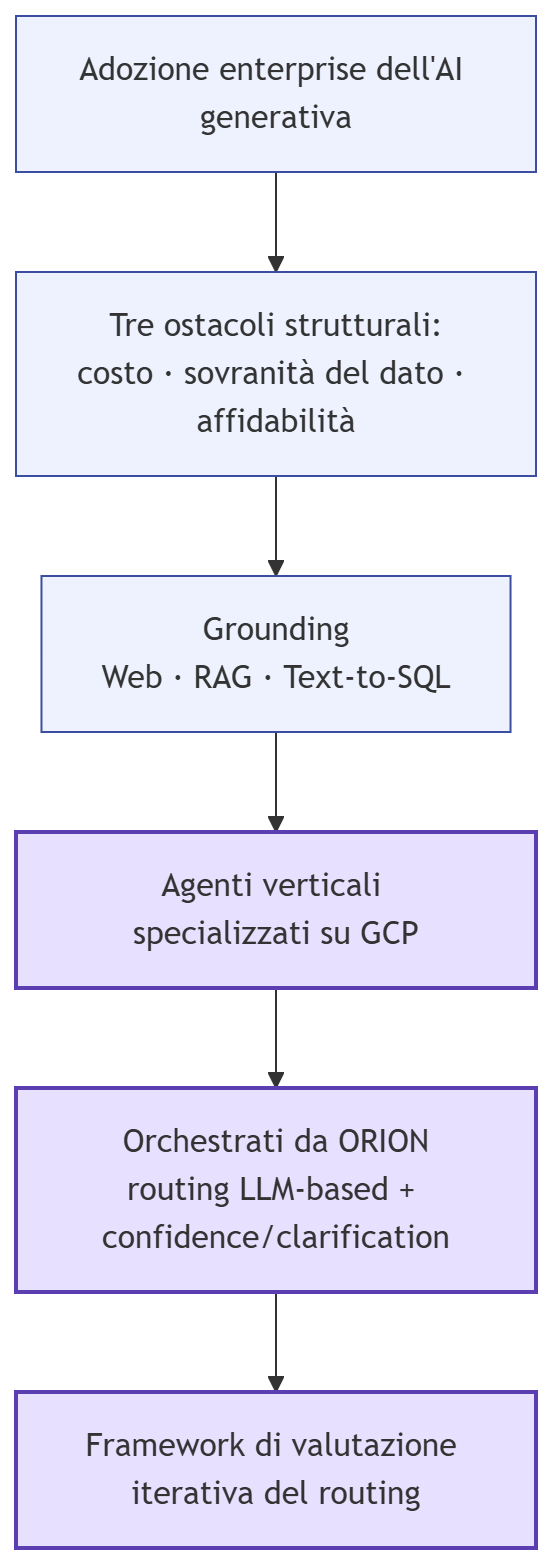
\includegraphics[height=0.85\textheight,keepaspectratio]{imbuto}
    \caption[Imbuto narrativo della tesi]{Imbuto narrativo: dal contesto generale dell'adozione enterprise dell'AI generativa ai contributi specifici di questo lavoro.}
    \label{fig:imbuto_narrativo}
\end{figure}

% =====================================================================
\section{Tre modi di ancorare un LLM alla realtà aziendale}
\label{sec:grounding-tre-modi}
% =====================================================================

La risposta al problema dell'allucinazione è il \emph{grounding}: l'ancoraggio della generazione del modello a fonti esterne verificabili, 
che forniscono al modello il contesto necessario per produrre risposte accurate. Il grounding opera a livello di inferenza (non modifica i pesi del modello) 
e si presenta in tre forme, ciascuna adeguata a un diverso tipo di fonte.

\paragraph{Web grounding.} Il modello accede ai risultati di un motore di ricerca per integrare informazioni attuali e pubbliche nella risposta.

\paragraph{Retrieval-Augmented Generation (RAG).} La domanda dell'utente è utilizzata per recuperare frammenti di documenti da un corpus indicizzato~\cite{lewis2020rag}; 
il modello genera la risposta vincolandosi a quel materiale.

\paragraph{Text-to-SQL.} La domanda è tradotta in una query SQL eseguita su un data warehouse; i risultati diventano il contesto per la generazione~\cite{yu2018spider,pourreza2023dinsql}.

I tre meccanismi sono descritti in dettaglio nel Capitolo~\ref{chap:background} (Sez.~\ref{sec:bg-grounding}).

La combinazione di queste tre tecniche di grounding \emph{all'interno di una stessa organizzazione} con l'ausilio di agenti specializzati per ciascun contesto 
e un meccanismo di coordinamento che li integri è una questione meno presente in letteratura, e costituisce il cuore di questa tesi.

% =====================================================================
\section{Il caso di studio}
\label{sec:caso-studio}
% =====================================================================

Il lavoro è stato svolto per intero nel contesto aziendale di
\href{https://www.coopalleanza3-0.it}{Coop Alleanza 3.0}, la 
\href{https://it.wikipedia.org/wiki/Coop_Alleanza_3.0}{più grande cooperativa di consumatori} del sistema Coop.
Lo stack IT dell'organizzazione comprende Google Cloud Platform come piattaforma cloud principale, 
Microsoft Entra ID come tenant identitario e SysAid come sistema di ticketing IT.

Per le ragioni citate (controllo dei costi, sovranità del dato, desiderio di avere una impronta etica che attenui il bias), è stato deciso dalla Cooperativa
di procedere con lo sviluppo di strumenti interni che consentano di sfruttare l'AI generativa alle proprie condizioni.

La domanda progettuale che ne deriva è: \emph{come si costruisce una piattaforma di AI generativa enterprise eterogenea, affidabile, economicamente sostenibile e sotto il pieno controllo dell'organizzazione?}

% =====================================================================
\section{Contributo e approccio}
\label{sec:contributi}
% =====================================================================

La tesi sostiene che la risposta è un'architettura ad \emph{agenti verticali specializzati}, 
ciascuno con la propria forma di grounding e il proprio dominio di competenza, 
\emph{coordinati da un orchestratore intelligente} 
che instrada dinamicamente le richieste dell'utente verso l'agente più appropriato.

I contributi specifici sono tre:

\begin{enumerate}
  \item \textbf{Progettazione e implementazione di una suite di agenti verticali su GCP.} 
  Quattro agenti specializzati: 
  Vera (generalista con Web grounding e RAG per-utente), CooPolicy (RAG su corpus documentale condiviso), 
  AllyCare (Text-to-SQL su dati NPS), SysAid (Text-to-SQL unificato con due fornitori di LLM) realizzati su infrastruttura cloud-native
  e dotati di autenticazione federata, catena di sicurezza e pipeline CI/CD. 
  Capitoli~\ref{chap:agenti-architettura} e~\ref{chap:agenti-implementazione}.

  \item \textbf{Progettazione, implementazione e valutazione dell'orchestrazione.} 
  Un orchestratore LLM-based che instrada le richieste sulla base di una stima di intento, complessità e confidenza, 
  con meccanismo di clarification quando l'ambiguità è alta. 
  La capacità generalista di Vera confluisce in Orion come opzione \texttt{self} (gestione delle richieste non specialistiche e fallback): 
  il router instrada quindi tra \texttt{self}, \texttt{sysaid}, \texttt{allycare} e \texttt{coopolicy}. 
  Capitoli~\ref{chap:orion-architettura} e~\ref{chap:orion-implementazione}.

  \item \textbf{Una metodologia di valutazione del routing.} 
  Basata su un gold standard configurabile e su un system prompt adattabile
  tramite interfaccia grafica per velocizzare le iterazioni e valutare velocemente
  le variazioni di performance.
  Capitolo~\ref{chap:orion-valutazione}.
\end{enumerate}

L'approccio si colloca nel filone della letteratura sui sistemi 
multi-agente basati su LLM~\cite{wu2023autogen,guo2024multiagent} 
e sul routing LLM~\cite{ong2024routellm}, con la specificità di un'implementazione 
completa e collocata in un contesto reale.

\begin{figure}[htbp]
    \centering
    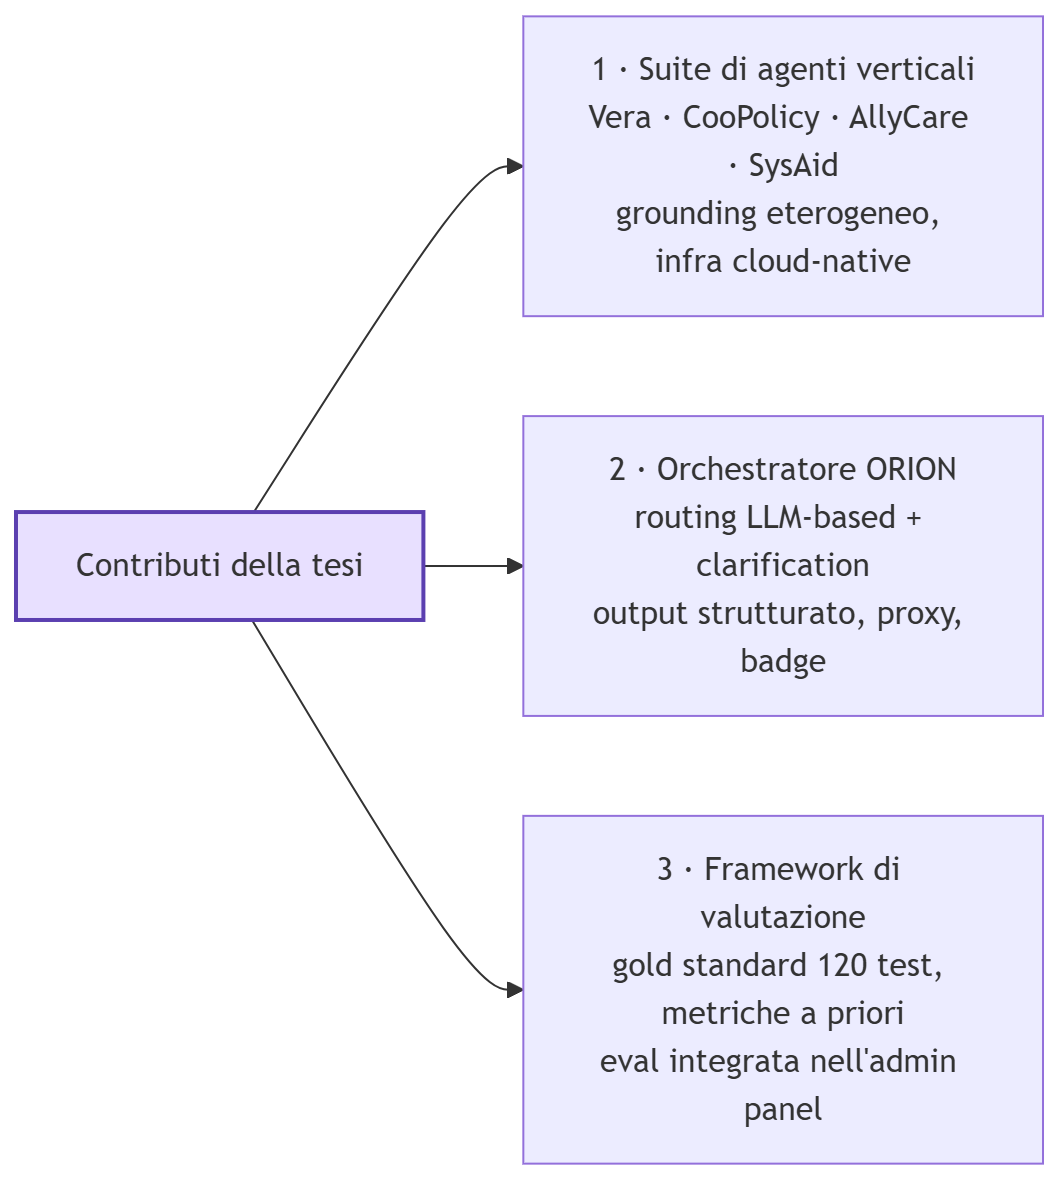
\includegraphics[width=0.7\textwidth,height=0.85\textheight,keepaspectratio]{contributi}
    \caption[Sintesi visuale dei contributi della tesi]{Sintesi visuale dei tre contributi: suite di agenti verticali, orchestratore, metodologia di valutazione del routing.}
    \label{fig:contributi_sintesi}
\end{figure}

% =====================================================================
\section{Cosa questa tesi \emph{non} è}
\label{sec:non-e}
% =====================================================================

È utile delimitare il perimetro del lavoro svolto e delle scelte fatte:

\begin{itemize}
  \item Questa tesi \textbf{non propone una nuova architettura di modello}. 
  I modelli utilizzati (Gemini, Claude) 
  sono servizi gestiti erogati da fornitori commerciali; il lavoro si concentra sul modo 
  in cui sono utilizzati, orchestrati e valutati.

  \item Questa tesi \textbf{non propone un nuovo algoritmo di routing appreso}. 
  Il routing in Orion è LLM-based (un modello che classifica le richieste), 
  non un classificatore addestrato su dati di preferenza. 
  L'alternativa appresa è discussa come direzione futura.

  \item Questa tesi \textbf{non sostiene che l'architettura proposta sia universalmente la risposta giusta}. 
  Mostra che lo è \emph{in questo contesto}, alla luce degli specifici vincoli esposti.

\end{itemize}

% =====================================================================
\section{Struttura della tesi}
\label{sec:struttura}
% =====================================================================

La tesi è organizzata in otto capitoli.

Il \textbf{Capitolo~\ref{chap:background}} introduce i concetti necessari per apprezzare i contributi: 
architettura Transformer, capacità e limiti degli LLM, prompt engineering e output strutturato, 
grounding nelle tre forme (Web, RAG, Text-to-SQL), 
architetture multi-agente, LLM routing, stima dell'incertezza, sicurezza e compliance, 
identity federation e infrastruttura cloud.

Il \textbf{Capitolo~\ref{chap:agenti-architettura}} presenta i principi guida 
e le scelte architetturali della suite di agenti verticali: 
principi etici, governance, agnosticità, sovranità del dato, 
modularità verticale, automazione dei rilasci e controllo degli accessi.

Il \textbf{Capitolo~\ref{chap:agenti-implementazione}} descrive l'implementazione della suite: 
stack tecnologico, organizzazione multi-repository, infrastruttura Terraform, 
pipeline CI/CD, catena di sicurezza e dettagli implementativi dei quattro agenti.

Il \textbf{Capitolo~\ref{chap:orion-architettura}} presenta l'architettura dell'orchestratore: motivazione, 
routing step con output strutturato, logica di confidence e clarification, 
agent proxy, gestione dell'identità e della storia conversazionale.

Il \textbf{Capitolo~\ref{chap:orion-implementazione}} descrive l'implementazione dell'orchestratore: 
router agent, agent proxy, endpoint di chat con routing integrato, 
frontend con badge trasparente, admin panel con pagina di valutazione, 
infrastruttura Terraform e schema del database.

Il \textbf{Capitolo~\ref{chap:orion-valutazione}} presenta la valutazione sperimentale su tre piani: 
il routing dell'orchestratore (domande di ricerca, gold standard, metriche dichiarate a priori, 
risultati e iterazione del prompt, analisi degli errori e limiti), 
la qualità dei sub-agenti (execution accuracy per gli agenti Text-to-SQL e faithfulness per il RAG) 
e una valutazione economica a ordini di grandezza.

Il \textbf{Capitolo~\ref{chap:conclusioni}} sintetizza i contributi, discute la generalizzabilità del pattern e presenta le direzioni di sviluppo futuro.

% =====================================================================
% CAPITOLO 2 — BACKGROUND
% =====================================================================
% Scopo (linee guida del prof): mettere un lettore non specialista
% (informatica magistrale) in condizione di apprezzare i contributi.
% Spiegare SOLO i concetti che riappaiono nei capitoli polpa.
% NON una rassegna esaustiva: una raccolta categorizzata costruita
% mentre si scrive la polpa.
%
% Ordine di scrittura: SECONDO (subito dopo la polpa).
% Lunghezza indicativa: ~25-30 pagine.
% =====================================================================

\chapter{Background}
\label{chap:background}

% TODO — Aprire il capitolo con un breve "manifesto" dello stile:
% spiegazione concisa, ogni sezione ancorata a 1-2 riferimenti
% bibliografici per l'approfondimento, niente di superfluo.

% =====================================================================
\section{Dai modelli di linguaggio ai Transformer}
\label{sec:bg-transformer}
% =====================================================================
% TODO — Richiamo storico SCURNO: n-gram -> RNN/LSTM -> attenzione ->
% Transformer \cite{vaswani2017attention}. Perche' il Transformer
% ha vinto: parallelizzazione, dipendenze a lungo raggio, scalabilita'.
% Distinzione encoder/decoder/encoder-decoder; dominanza decoder-only
% (GPT, LLaMA, Gemini, Claude).

% =====================================================================
\section{Large Language Model: capacita', limiti, allineamento}
\label{sec:bg-llm}
% =====================================================================
% TODO — Pre-training autoregressivo, capacita' emergenti, leggi di scala
% \cite{brown2020gpt3}. Instruction tuning + RLHF \cite{ouyang2022instructgpt}
% come allineamento al comportamento desiderato.
% Allucinazioni come limite strutturale \cite{xu2024hallucination}.
% Knowledge cutoff e conseguenze pratiche in azienda.

% =====================================================================
\section{Prompt engineering, function calling, tool use}
\label{sec:bg-prompting}
% =====================================================================
% TODO — Zero-shot, few-shot, Chain-of-Thought \cite{wei2022cot}.
% Function calling: schema, agentic loop, tool nidificati.
% E' il meccanismo su cui si fondano gli agenti Text-to-SQL e il router
% di Orion (output strutturato).

% =====================================================================
\section{Grounding: ancorare la generazione a fonti esterne}
\label{sec:bg-grounding}
% =====================================================================
% TODO — Il grounding come contromisura alle allucinazioni
% \cite{guu2020realm}. Differenza concettuale tra grounding (intervento
% a inferenza) e fine-tuning (modifica dei pesi).

% [FIGURA 2.1] Tre meccanismi di grounding affiancati: Web grounding,
% RAG, Text-to-SQL — uno schema che mostri input, fonte ancorata, output.
% Tipo: schema concettuale.
%
% \begin{figure}[h]
%     \centering
%     \includegraphics[width=0.95\textwidth]{fig02_grounding_three_ways.pdf}
%     \caption[Tre forme di grounding affiancate]{Tre meccanismi di grounding adottati nella suite: Web grounding (Vera), RAG (CooPolicy) e Text-to-SQL (AllyCare, SysAid).}
%     \label{fig:grounding_three_ways}
% \end{figure}

\subsection{Web grounding}
\label{subsec:bg-web-grounding}
% TODO — Integrazione nativa Google Search in Vertex AI. Quando
% e' appropriato (fatti pubblici, attualita') e quando NO (dati privati).

\subsection{Retrieval-Augmented Generation}
\label{subsec:bg-rag}
% TODO — Pipeline canonica \cite{lewis2020rag}: chunking, embedding,
% vector store, retrieval, generation. Hybrid search dense+sparse,
% re-ranking, query expansion \cite{ma2023query_expansion},
% HyDE \cite{gao2022hyde}. Vertex AI RAG Engine come realizzazione managed.
% Distinzione cruciale (riusata in Cap. 3): RAG corpus per-utente
% vs RAG corpus condiviso.

% [FIGURA 2.2] Pipeline RAG canonica: documento -> chunk -> embedding ->
% indice -> retrieval -> generation con contesto.
%
% \begin{figure}[h]
%     \centering
%     \includegraphics[width=0.9\textwidth]{fig02_rag_pipeline.pdf}
%     \caption[Pipeline RAG canonica]{Pipeline canonica di Retrieval-Augmented Generation: dall'ingestione dei documenti alla generazione vincolata al contesto recuperato.}
%     \label{fig:rag_pipeline}
% \end{figure}

\subsection{Text-to-SQL}
\label{subsec:bg-text2sql}
% TODO — Traduzione NL -> SQL. Challenge: schema awareness, dialetti,
% JOIN multi-tabella, aggregazioni temporali. Benchmark: Spider
% \cite{yu2018spider}, BIRD \cite{li2023bird}. Metriche: execution
% accuracy, exact match. Approcci con LLM: schema injection, few-shot,
% decomposizione \cite{pourreza2023dinsql}.

% =====================================================================
\section{Valutazione automatica di sistemi RAG: il framework RAGAS}
\label{sec:bg-ragas}
% =====================================================================
% TODO — RAGAS \cite{es2023ragas} come insieme di metriche LLM-as-judge:
% faithfulness, answer relevancy, context precision, context recall.
% Limiti del paradigma LLM-as-judge \cite{zheng2023llmjudge}.

% =====================================================================
\section{Agenti LLM e architetture multi-agente}
\label{sec:bg-multiagent}
% =====================================================================
% TODO — Paradigma ReAct \cite{yao2022react} (Thought -> Action -> Observation),
% memoria short/long-term. Survey LLM multi-agente \cite{guo2024multiagent}:
% architetture cooperative, competitive, hierarchical.
% Orion = hierarchical con supervisor agent.
% Pattern AutoGen \cite{wu2023autogen}: GroupChatManager.
% Mixture-of-Agents \cite{wang2024moa} come riferimento terminologicamente
% piu' corretto del classico MoE \cite{jiang2024mixtral} (interno al modello).

% [FIGURA 2.3] Tassonomia architetture multi-agent (cooperative,
% hierarchical, competitive) con esempi di pattern.
%
% \begin{figure}[h]
%     \centering
%     \includegraphics[width=0.85\textwidth]{fig02_multiagent_taxonomy.pdf}
%     \caption[Tassonomia delle architetture multi-agent LLM]{Le tre macro-categorie di architetture multi-agent secondo \cite{guo2024multiagent}, con il posizionamento di Orion nel ramo \emph{hierarchical}.}
%     \label{fig:multiagent_taxonomy}
% \end{figure}

% [FIGURA 2.4] Pattern ReAct: ciclo Thought -> Action -> Observation.
%
% \begin{figure}[h]
%     \centering
%     \includegraphics[width=0.7\textwidth]{fig02_react_loop.pdf}
%     \caption[Ciclo ReAct]{Il ciclo Thought-Action-Observation del pattern ReAct \cite{yao2022react}, alla base degli agenti della suite e del router di Orion.}
%     \label{fig:react_loop}
% \end{figure}

% =====================================================================
\section{LLM routing e ottimizzazione costo--qualita'}
\label{sec:bg-routing}
% =====================================================================
% TODO — Cost-quality trade-off. FrugalGPT \cite{chen2023frugalgpt}:
% LLM cascade, early-exit basato su confidenza. RouteLLM \cite{ong2024routellm}:
% formalizzazione del routing come classificazione strong/weak,
% confronto Matrix Factorization / BERT classifier / Causal LLM /
% SW Ranking. Metodologia di valutazione MMLU/MT-Bench.
%
% Posizionare il router di Orion nel quadro: e' un LLM-based router
% (Gemini Flash) con output strutturato, NON un modello appreso.

% =====================================================================
\section{Stima dell'incertezza e confidence calibration}
\label{sec:bg-confidence}
% =====================================================================
% TODO — Capacita' degli LLM di sapere di non sapere
% \cite{kadavath2022knowsknows}. Self-consistency \cite{wang2022selfconsistency}
% come proxy di confidenza (costoso). Active learning \cite{settles2012active}
% come fondamento del meccanismo di clarification di Orion: il sistema
% interroga l'oracolo (utente) solo quando l'informazione aggiuntiva
% ha massimo valore.

% =====================================================================
\section{Sicurezza, privacy, compliance}
\label{sec:bg-security}
% =====================================================================
% TODO — Model Armor: filtri Responsible AI e difese contro prompt
% injection \cite{perez2022promptinjection}. Cloud DLP: PII con info types
% standard e custom (Codice Fiscale, Partita IVA, IBAN per il contesto
% italiano).

% =====================================================================
\section{Identity federation}
\label{sec:bg-identity}
% =====================================================================
% TODO — OAuth 2.0 \cite{rfc6749oauth2}, OpenID Connect \cite{oidc1_0core},
% JWT \cite{rfc7519jwt}. Microsoft Entra ID e MSAL come implementazione
% adottata in Coop.

% =====================================================================
\section{Infrastruttura cloud}
\label{sec:bg-cloud}
% =====================================================================
% TODO — Cloud Run come piattaforma serverless container.
% Cloud SQL + Private Service Connect. Vertex AI: catalogo modelli +
% RAG Engine + Grounding. Terraform come Infrastructure-as-Code.
% Citare la documentazione ufficiale: \cite{gcp_cloudrun},
% \cite{gcp_vertexai}, \cite{terraform_docs}.

% !TEX root = ../main.tex
% =====================================================================
% CAPITOLO 3 — LA SUITE DI AGENTI VERTICALI
% =====================================================================

\chapter{La suite di agenti verticali}
\label{chap:agenti}

Questo capitolo descrive la prima fase del progetto: la progettazione e la
realizzazione della suite di agenti verticali. Il percorso segue l'ordine
delle decisioni effettivamente prese: per primi i principi guida che hanno
condizionato ogni scelta successiva e l'architettura d'insieme che ne
deriva; quindi le fondazioni trasversali comuni a tutti i servizi (stack
tecnologico, organizzazione del codice, infrastruttura come codice, identità
e sicurezza) e infine il dettaglio di ciascuno dei quattro agenti. 
Chiudono il capitolo il
pannello di amministrazione e le alternative progettuali considerate e
scartate.

% =====================================================================
\section{Principi guida}
\label{sec:agenti-principi}
% =====================================================================
\label{subsec:agenti-principi-guida}

La progettazione è stata guidata da una serie di fondamenti trasversali,
stabiliti prima di avviare lo sviluppo e mantenuti durante le fasi successive.

\begin{description}

  \item[Rispetto dei principi etici e cooperativi]
    Gli agenti LLM sono intrinsecamente portati a esprimere bias (Sez.~\ref{sec:bg-llm}).
    Sviluppando agenti interni, il  "comportamento" (definito da guardrail 
    e prompt di sistema) si può definite collegialmente fra gli uffici interni (Etica, Sicurezza IT),
    integrando direttive esplicite che allineano ogni agente all'identità e ai valori
    della cooperativa e in conformità con i requisiti di trasparenza e \emph{human oversight}
    dell'European AI Act~\cite{eu2024aiact}, con cicli di aggiornamento rapidi e controllati.
    Inoltre, offrire un pacchetto di assistenti interni mitiga questo previene il
    ricorso incontrollato a strumenti AI esterni non autorizzati (\emph{Shadow AI}), riducendo i rischi per
    la sicurezza del dato.

  \item[Governance facilitata e efficace]
    Le configurazioni del prompt di sistema (la ``personalità'' dell'agente) e i controlli su
    utilizzi impropri o sensibili devono essere configurabili da una dashboard apposita, 
    usabile anche dagli uffici preposti privi di competenza tecnica, che consenta inoltre di monitorare
    gli eventi segnalati come ``pericolosi''. Tutto il codice sorgente risiede nel repository 
    Git della Cooperativa ed è di sua proprietà.

  \item[Implementazione agnostica e sostenibile]
    Le soluzioni AI ``out of the box'' dei fornitori commerciali comportano spesso \emph{vendor lock-in}
    (difficile portabilità verso altre infrastrutture) e costi fissi di sottoscrizione anche con
    utilizzo scarso. La soluzione realizzata vuole invece essere portabile verso qualunque
    architettura o fornitore di LLM e consentire un controllo dinamico dei costi: un budget di utilizzo (``token'')
    per utente, definito dagli amministratori e modificabile alla bisogna, e ovunque possibile un
    \emph{routing} che indirizzi le richieste a bassa complessità verso modelli più economici.

  \item[Sovranità del dato]
    Nessun dato deve lasciare il perimetro cloud europeo, in conformità al Regolamento Generale sulla Protezione dei Dati (GDPR).

  \item[Modularità verticale]
    Ogni dominio informativo o funzionale deve essere affidato a un agente autonomo e indipendente,
    con il proprio meccanismo di grounding, il proprio ciclo di vita applicativo e la propria infrastruttura di deployment:
    in modo che sia possibile effettuare \emph{prompt engineering} e \emph{few-shot learning}~\cite{brown2020gpt3}
    ad hoc per il singolo caso d'uso.
    I sistemi devono essere il più possibile isolati per consentire di aggiornare, monitorare e
    scalare ogni servizio in modo indipendente.

  \item[Automazione dei rilasci]
    Le evolutive o correzioni di bug devono potere essere rilasciate in maniera trasparente verso l'utente 
    senza causare disservizio,
    in maniera automatizzata per ridurre al minimo la possibilità di errore umano,
    e con uno step approvativo per il passaggio in produzione.

  \item[Accesso privato e con controllo centralizzato]
    L'intero ecosistema deve potere essere accessibile solo da rete interna o VPN di Coop Alleanza:
    l'infrastruttura utilizzata deve quindi evitare l'esposizione su rete pubblica.
    Il controllo dell'abilitazione degli utenti all'uso degli assistenti deve integrarsi con il sistema di Identity Management
    già esistente nell'organizzazione, basato sui protocolli OAuth~2.0~\cite{rfc6749oauth2} e OpenID Connect~\cite{oidc1_0core}
    su Microsoft Entra ID~\cite{msft_entra_id}.

\end{description}

% =====================================================================
\section{Architettura d'insieme}
\label{subsec:agenti-architettura-insieme}
% =====================================================================

L'ecosistema è accessibile da un unico ``portale'', per consentire modularità: 
eventuali nuovi agenti si innestano nel \emph{framework} esistente, così
che l'utente finale possa accedervi in maniera pratica e intuitiva.

Pur restando centrale il principio di agnosticità e portabilità, tutte le implementazioni usano
la piattaforma Cloud di Google~\cite{gcp_vertexai,gcp_cloudrun}, al momento l'unico fornitore
attivo in Coop Alleanza e adeguato alle necessità.

\begin{figure}[htbp]
  \centering
  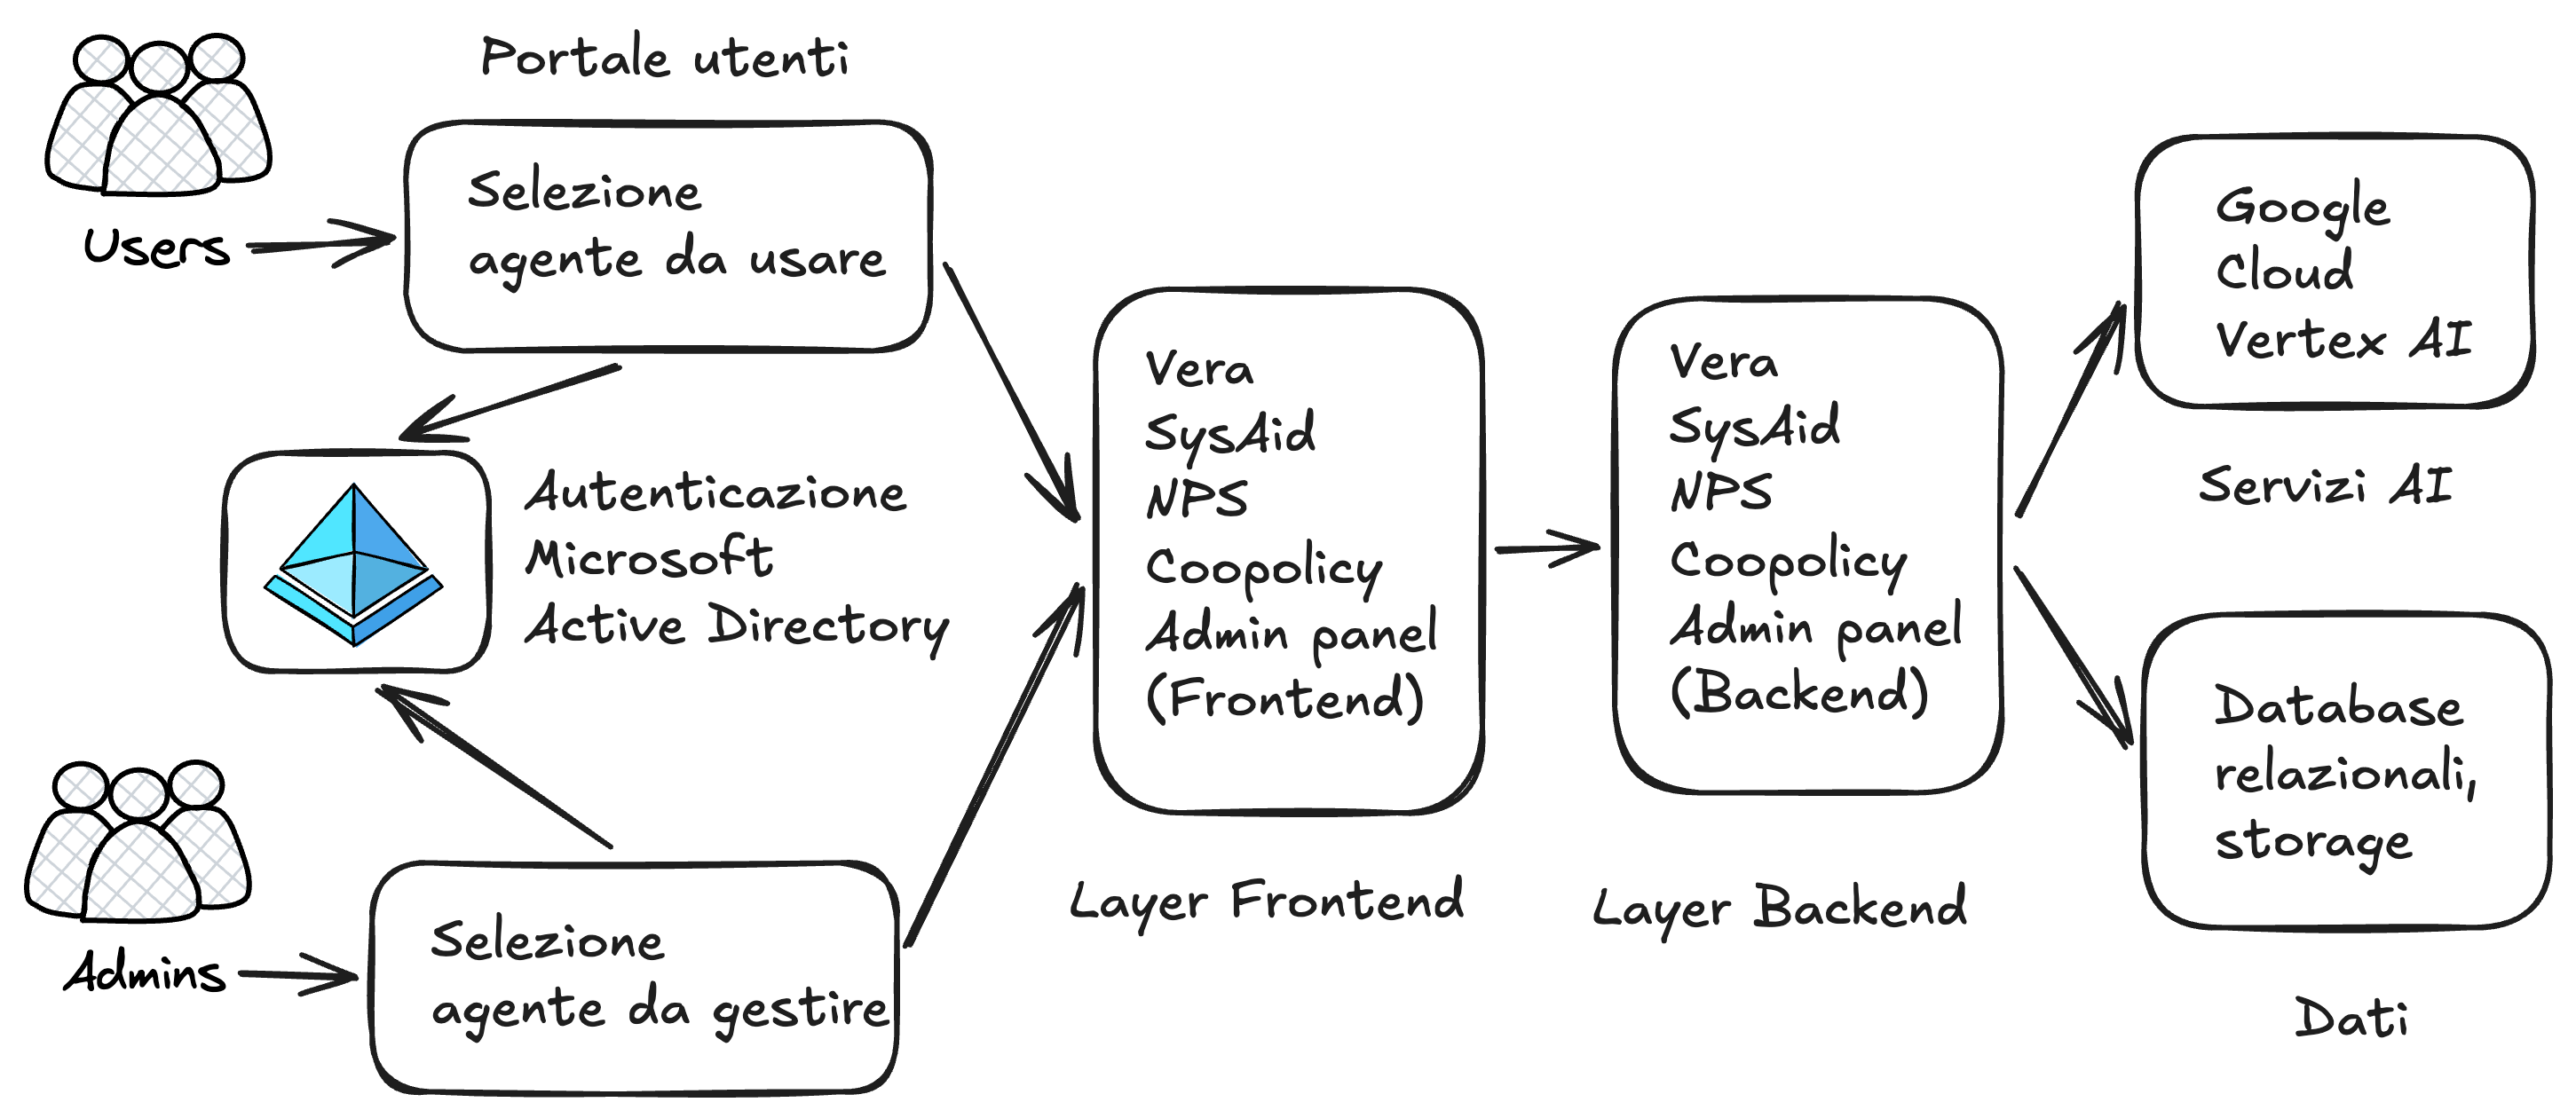
\includegraphics[width=0.9\textwidth]{fig1}
  \caption[Architettura d'insieme della suite di agenti]{Architettura
    della suite di agenti verticali: portal con autenticazione federata,
    istanze serverless indipendenti e infrastruttura
    condivisa per database, data warehouse e servizi AI.}
  \label{fig:architettura_suite}
\end{figure}

% =====================================================================
\section{Fondazioni trasversali: stack, infrastruttura, sicurezza}
\label{sec:agenti-stack}
% =====================================================================

Prima di esaminare i singoli agenti, questa sezione descrive gli elementi
trasversali del progetto,presentati qui una sola volta: l
o stack tecnologico, l'organizzazione del
codice, l'infrastruttura come codice con la pipeline di rilascio, e il
modello di identità e autorizzazione.

\subsection{Stack tecnologico}
\label{subsec:agenti-stack-tech}

L'implementazione dell'ecosistema di agenti è basata su uno stack cloud-native
 omogeneo per minimizzare la diversità fra servizi (riducendo la complessità
per quanto possibile) e per delegare ai \emph{managed services} di Google Cloud Platform tutti i compiti
infrastrutturali.

\begin{itemize}
  \item \textbf{Backend.} Tutti gli agenti sono scritti in Python~3.10+ ed
        esposti tramite il framework asincrono FastAPI~\cite{fastapi_docs}. 
        La scelta è motivata
        dalla natura prevalentemente \emph{I/O bound} delle interazioni con i
        Large Language Model: la generazione di una risposta richiede da
        centinaia di millisecondi a decine di secondi, quasi interamente spesi
        in attesa del modello, dei motori di retrieval o di BigQuery. Il modello
        di concorrenza \texttt{async/await} consente di sostenere centinaia di
        richieste concorrenti per istanza Cloud Run senza ricorrere a
        thread o processi multipli. L'accesso al database relazionale avviene
        in modo asincrono tramite SQLAlchemy~2 e il driver
        \texttt{asyncpg}, con \emph{pool} pre-pingati e ricicli automatici.
  \item \textbf{Frontend.} Le interfacce sono React~19 con TypeScript,
        impacchettate con Vite e stilizzate con Tailwind~CSS. La scelta
        di un \emph{bundler} ESM moderno è funzionale alla pipeline CI/CD:
        il build è di pochi secondi, riducendo i tempi di rilascio.
  \item \textbf{Database e Data Warehouse.} Cloud SQL per
        PostgreSQL~15~\cite{gcp_cloudsql} è il \emph{system of record}
        applicativo: vi risiedono utenti, conversazioni, messaggi, quote,
        ACL, audit log e parametri di configurazione. Google
        BigQuery~\cite{gcp_bigquery} è invece il database analitico
        utilizzato dagli agenti Text-to-SQL (AllyCare e SysAid), con
        dataset alimentati in modo continuo da flussi appositi.
  \item \textbf{Large Language Models.} L'implementazione poggia su due
        famiglie di modelli erogati come \emph{managed APIs}: Gemini~2.5
        Flash e Pro~\cite{team2024gemini} su Vertex AI~\cite{gcp_vertexai},
        e Claude Sonnet~4.6~\cite{anthropic2024claude}
        attraverso l'SDK Anthropic veicolato dal canale
        \texttt{AnthropicVertex}~\cite{anthropic_docs}. La coesistenza
        dei due fornitori in SysAid (Sez.~\ref{sec:agenti-sysaid-arch})
        concretizza un caso di agnosticità come richiesto dai principi
        guida (Sez.~\ref{sec:agenti-principi}).
  \item \textbf{Sviluppo di agenti.} Viene utilizzato il \emph{Google Agent
        Development Kit}~(ADK)~\cite{google_adk_docs}, una libreria aperta,
        ufficiale e portabile che astrae la gestione della sessione, l'invocazione
        ciclica del modello e l'integrazione di \emph{tool} basati su
        \emph{function calling}.
 \item \textbf{Infrastruttura.} Ogni componente applicativo è un servizio
        serverless eseguito su Google Cloud Run~\cite{gcp_cloudrun},
        descritto interamente da codice Terraform~\cite{terraform_docs}.
\end{itemize}

\subsection{Organizzazione del codice}
\label{subsec:agenti-multirepo}

Il codice sorgente dell'intera suite è organizzato in repository Git distinti
(Fig.~\ref{fig:multirepo_tree}), ciascuno autonomo e con il proprio ciclo di
vita, e raccolti in un unico progetto Bitbucket (Fig.~\ref{fig:progetto_bitbucket}). Ogni repository
contiene il proprio \texttt{Dockerfile}, le proprie dipendenze e il proprio
file di descrizione della pipeline (\texttt{cloudbuild.yaml}),
ed è collegato a un trigger Cloud Build dedicato. Questa separazione consente
rilasci indipendenti: un aggiornamento a CooPolicy non richiede il rebuild
di Vera, e un hotfix su SysAid può essere rilasciato senza coordinamento
con il frontend del portale. I branch \texttt{test} e \texttt{main} di ogni
repository corrispondono rispettivamente all'ambiente di collaudo e a quello
di produzione; il branch develop può invece essere sfruttato per i test in locale.

\begin{figure}[h]
  \centering
  \begin{lstlisting}[language=bash]
vera-backend/              # Vera Backend (FastAPI + ADK + Gemini)
vera-frontend/             # Vera Frontend (React)
vera-admin-backend/        # Pannello amministrativo di Vera Backend
vera-admin-frontend/       # Pannello amministrativo di Vera Frontend
sysaid-backend/            # SysAid Backend unificato (Gemini + Sonnet)
sysaid-frontend/           # SysAid Frontend
coopolicy-backend/         # CooPolicy Backend (FastAPI + RAG)
coopolicy-frontend/        # CooPolicy Frontend
allycare-backend/          # AllyCare Backend (FastAPI + ADK + BigQuery)
allycare-frontend/         # AllyCare Frontend
portal-frontend/           # Portale utenti (MSAL)
admin-portal-frontend/     # Portale amministrativo
infrastructure/            # Terraform per infrastruttura
  \end{lstlisting}
  \caption[Elenco dei repository della suite (agenti)]{Elenco dei repository della suite nella ``fase'' degli agenti verticali. Ogni servizio è un progetto Git autonomo con proprio ciclo di CI/CD e branch per ambiente (\texttt{test}, \texttt{main}). I repository dell'orchestratore sono inseriti dal Capitolo~\ref{chap:orion}.}
  \label{fig:multirepo_tree}
\end{figure}

\begin{figure}[htbp]
  \centering
  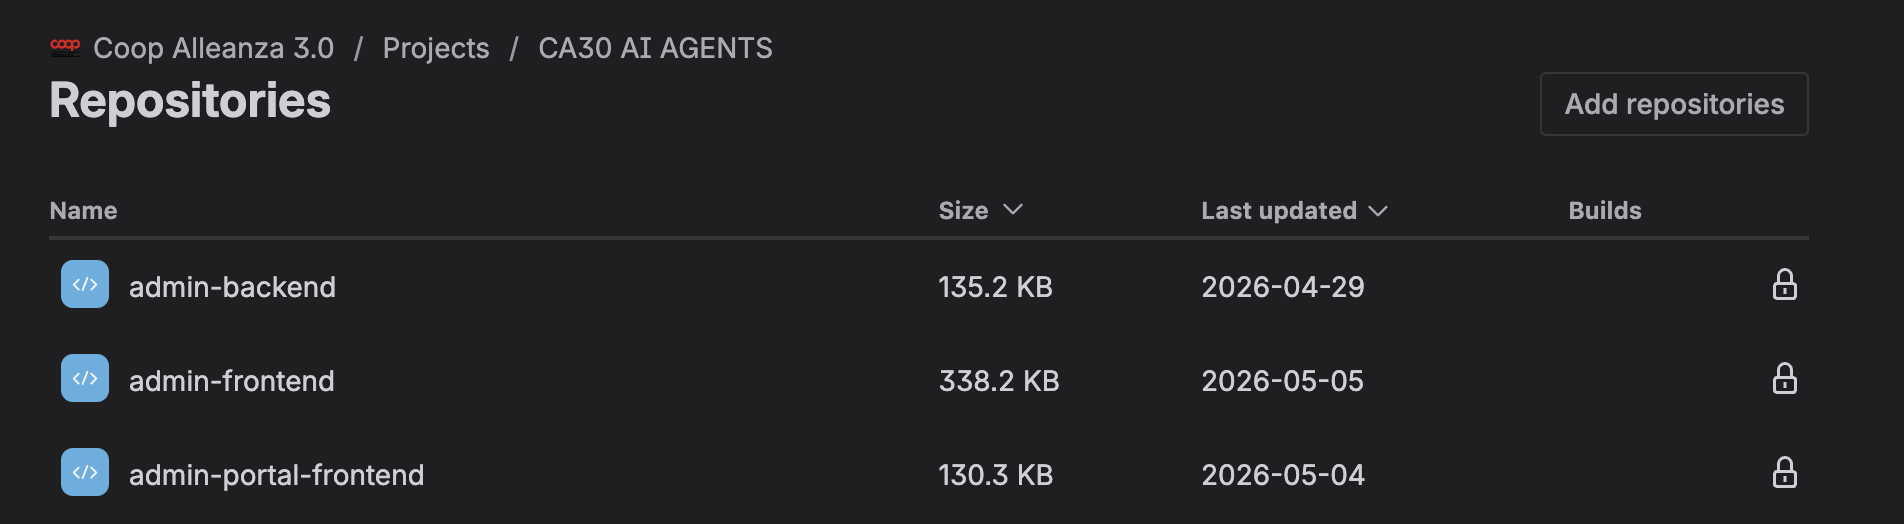
\includegraphics[width=0.9\textwidth]{progetto-bitbucket}
  \caption[Progetto Bitbucket della suite]{Il progetto Bitbucket che raccoglie i repository della suite: ogni servizio è un repository autonomo con il proprio ciclo di CI/CD.}
  \label{fig:progetto_bitbucket}
\end{figure}

I backend più complessi (Vera e Vera-Admin) adottano una separazione interna del codice
più strutturata: la directory \texttt{api/} contiene esclusivamente i router
FastAPI; \texttt{services/} le funzioni di dominio prive di stato HTTP;
\texttt{models/} le entit\`a SQLAlchemy; \texttt{schemas/} i modelli Pydantic
per validazione di input e output; \texttt{core/} le utility trasversali
(database, dipendenze, sicurezza). I backend più piccoli (CooPolicy, AllyCare e
SysAid) condividono la stessa filosofia in forma compressa, con
un singolo \texttt{main.py} che monta i \emph{router} e alcuni moduli
ausiliari (\texttt{auth.py}, \texttt{tools.py}, \texttt{agent.py}, \texttt{quote.py}).

\subsection{Infrastruttura come codice e pipeline CI/CD}
\label{subsec:agenti-iac}

L'intera infrastruttura GCP è descritta in Terraform~\cite{terraform_docs} (Fig.~\ref{fig:arch_terraform}) ed è
parametrizzata su due ambienti, \texttt{test} e \texttt{prod}, gestiti come
progetti indipendenti con \emph{state} remoto su un bucket Cloud
Storage. Le risorse provisionate comprendono: l'abilitazione delle API GCP
necessarie, le istanze Cloud Run con un service account condiviso, l'istanza
Cloud SQL con il relativo \emph{Private Service Connect} consumer endpoint, le
politiche di Identity and Access Management (IAM), il bucket di Artifact
Registry per le immagini Docker, il template Model Armor, la rete (subnet,
indirizzi IP riservati, regole di forwarding) e il bilanciatore di carico HTTPS
interno con il certificato TLS recuperato da Secret Manager (Certificato fornito dall'IT di Coop Alleanza).

Le decisioni di sicurezza fondamentali sono codificate direttamente nel
modulo Terraform e dunque non sono modificabili senza una \emph{pull request}
revisionata:

\begin{enumerate}
  \item \textbf{Egress limitato a indirizzi privati.} Ogni servizio Cloud Run
        è collegato alla VPC interna mediante \emph{Direct VPC Egress} con
        \texttt{egress = PRIVATE\_RANGES\_ONLY}: il container può raggiungere
        gli endpoint privati GCP (Vertex AI, BigQuery, Cloud SQL, RAG Engine)
        ma non internet pubblico. Il vincolo è particolarmente importante per
        gli agenti Text-to-SQL e per Vera, dove un'eventuale estrazione di dati verso
        l'esterno via DNS o webhook è di fatto resa impossibile a livello di
        rete.
  \item \textbf{Database non esposto su IP pubblico.} L'istanza Cloud SQL ha
        \texttt{ipv4\_enabled = false}: la connessione passa solo attraverso
        \emph{Private Service Connect} (PSC), con un \emph{forwarding rule}
        regionale verso il \emph{service attachment} di Cloud SQL:
        è, in sostanza, anch'esso esposto in sola rete privata.
  \item \textbf{Bilanciatore di carico interno.} Il \emph{frontend} è
        accessibile solo via un \emph{Application Load Balancer regionale
        interno} (\texttt{INTERNAL\_MANAGED}). L'esposizione
        avviene perciò solo all'interno della rete aziendale o, per gli
        utenti remoti, dietro VPN, soddisfacendo il requisito di
        accesso privato (Sez.~\ref{sec:agenti-principi}).
  \item \textbf{Segregazione di credenziali.} Tutte le password generate
        (database, JWT) sono prodotte da \texttt{random\_password},
        depositate in Secret Manager e iniettate nei container via
        \texttt{value\_source.secret\_key\_ref}: nessun segreto
        attraversa mai il file system dello sviluppatore.
\end{enumerate}

\begin{figure}[htbp]
  \centering
  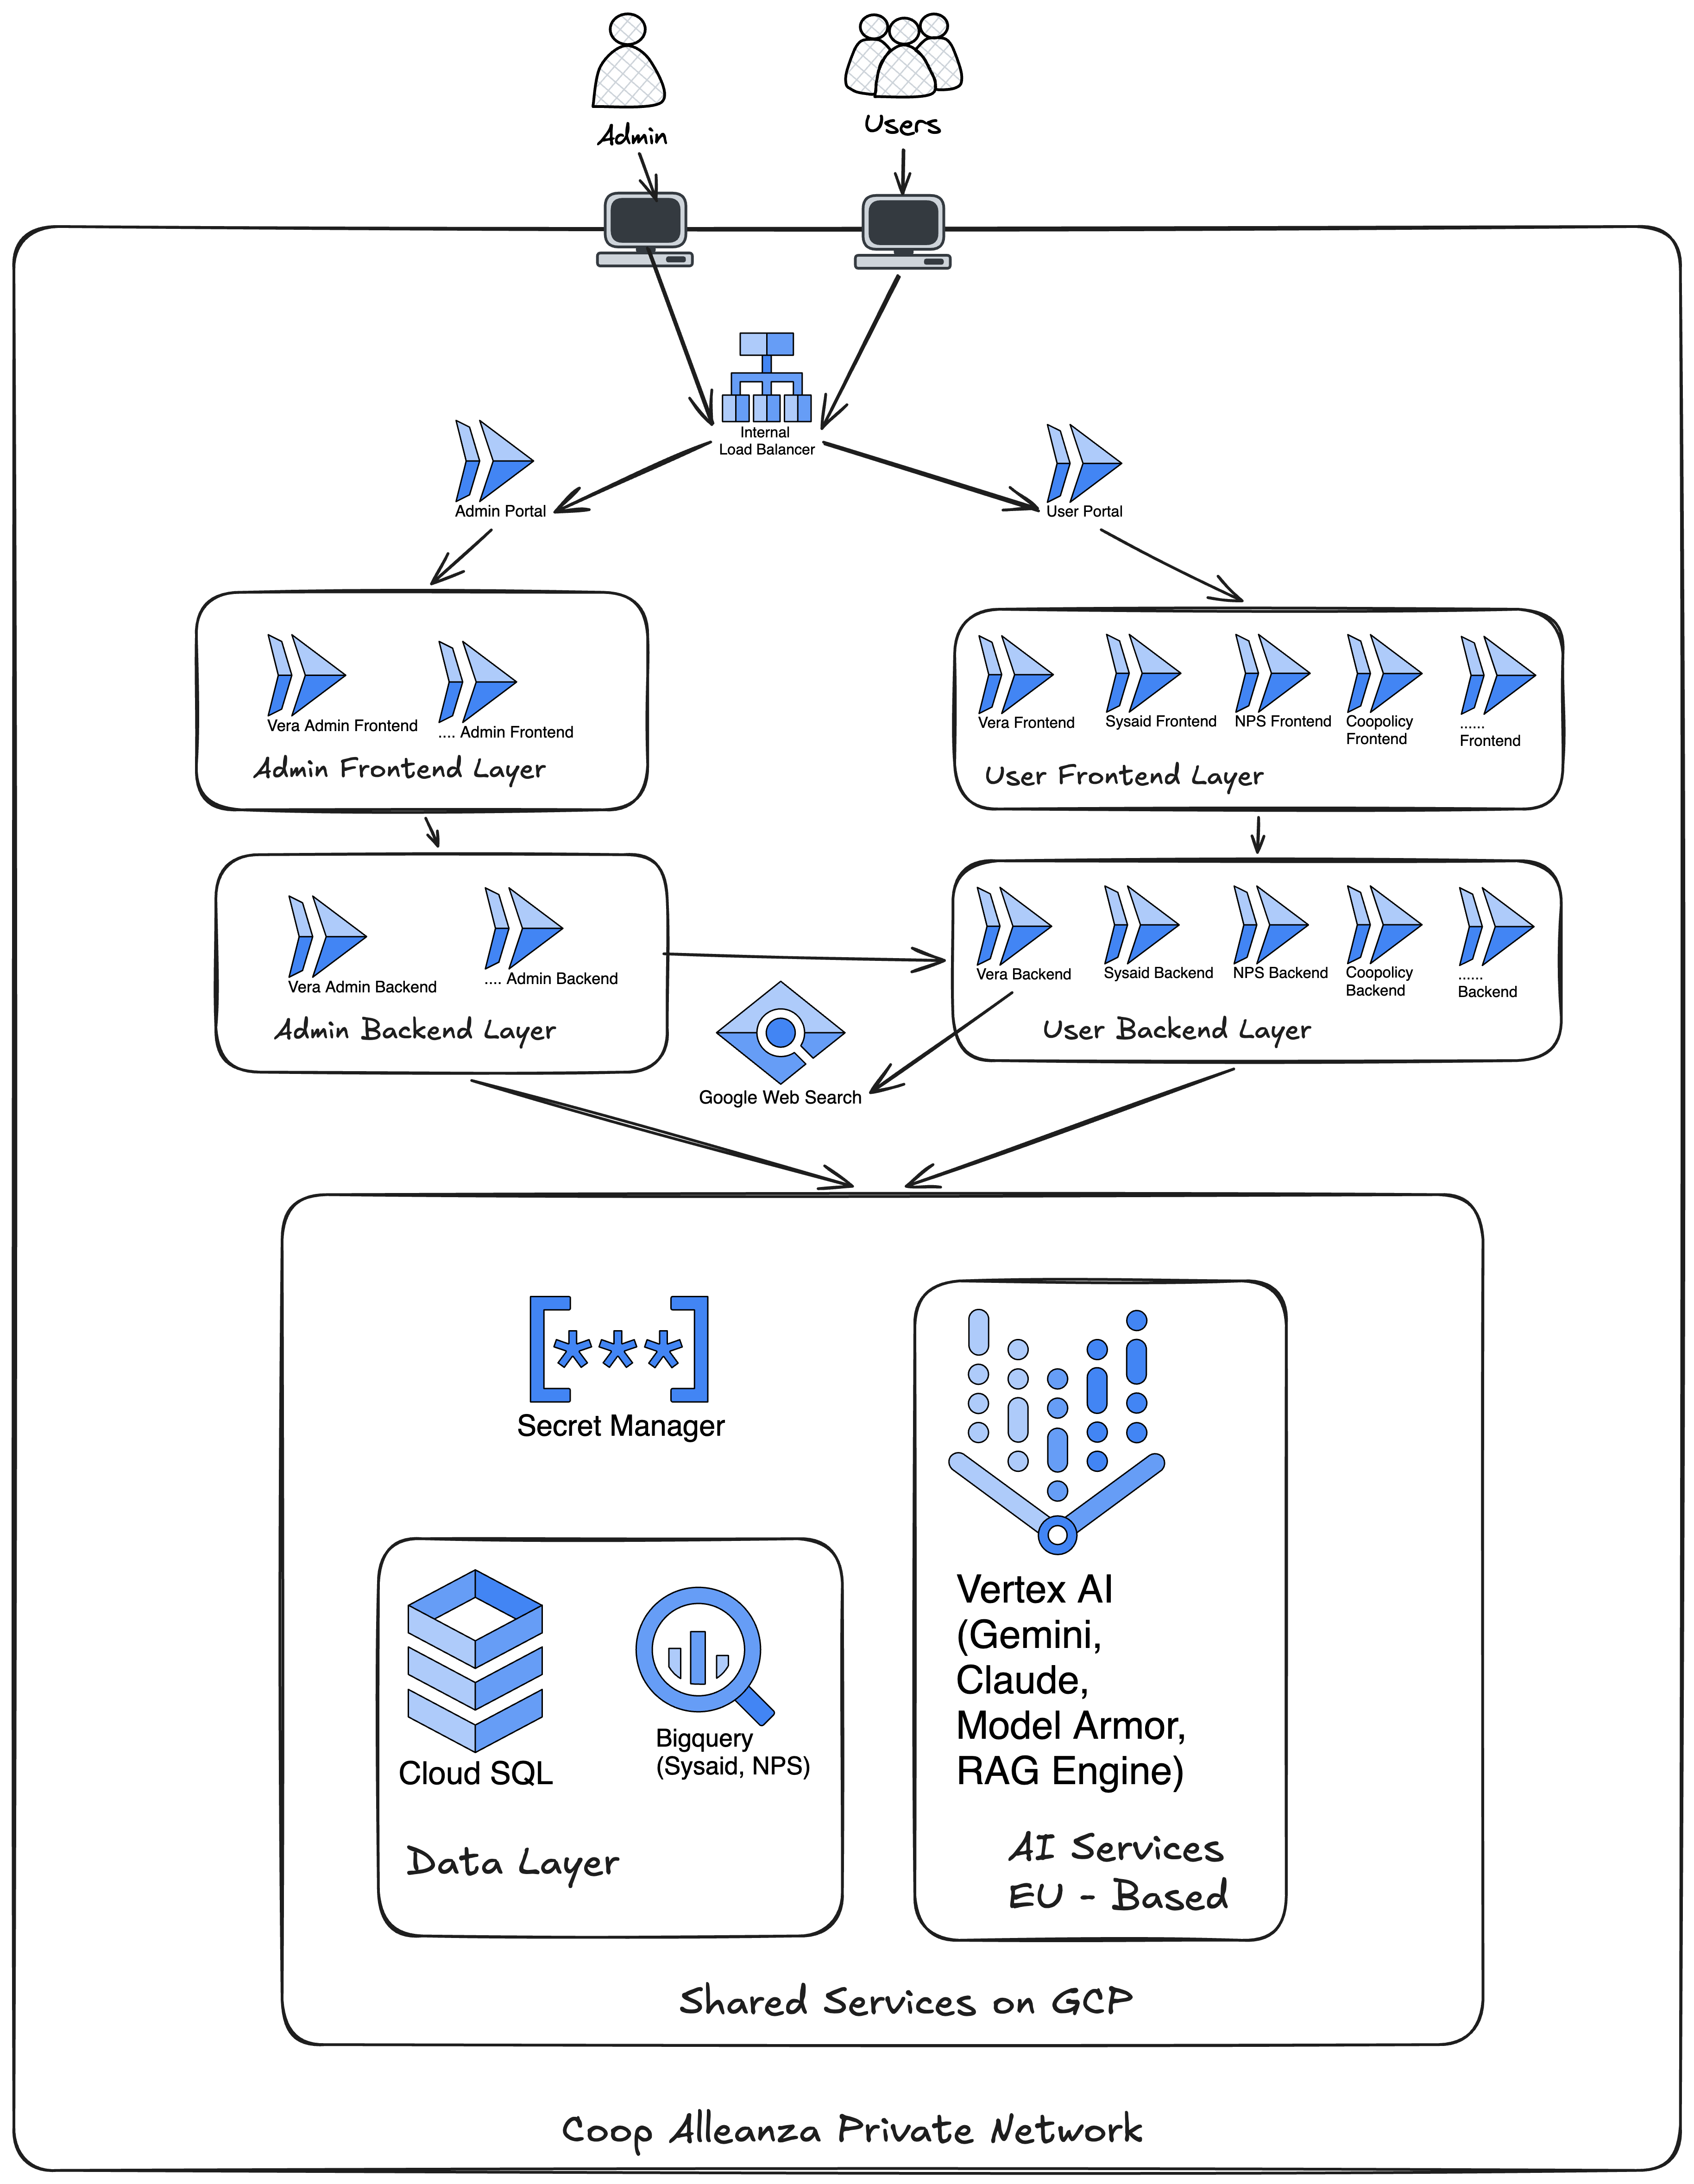
\includegraphics[width=0.9\textwidth]{arch-terraform}
  \caption[Architettura GCP descritta in Terraform]{Architettura completa dell'infrastruttura GCP della suite, così come descritta nei moduli Terraform: Cloud Run, Cloud SQL, Load Balancer interno, Secret Manager, Vertex AI.}
  \label{fig:arch_terraform}
\end{figure}

La pipeline CI/CD (Fig.~\ref{fig:cicd_pipeline}) si attiva ad ogni \emph{push}: in ambiente di test sul branch
\texttt{test}, in produzione sul branch \texttt{main}. Cloud Build, configurato
tramite un \emph{trigger} per ciascun servizio collegato al rispettivo
repository Bitbucket, esegue i passi descritti nel \texttt{cloudbuild.yaml}
locale: build dell'immagine Docker, push su Artifact Registry e aggiornamento
dell'immagine attiva del relativo servizio Cloud Run. Per l'ambiente di
produzione, il \emph{trigger} ha \texttt{approval\_required = true}, che
implementa lo step approvativo richiesto dal principio di
\emph{Automazione dei rilasci} (Sez.~\ref{sec:agenti-principi}).
Tale rilascio potrà essere poi ``sbloccato'' solo dagli amministratori di sistema della Cooperativa.

\begin{figure}[htbp]
  \centering
  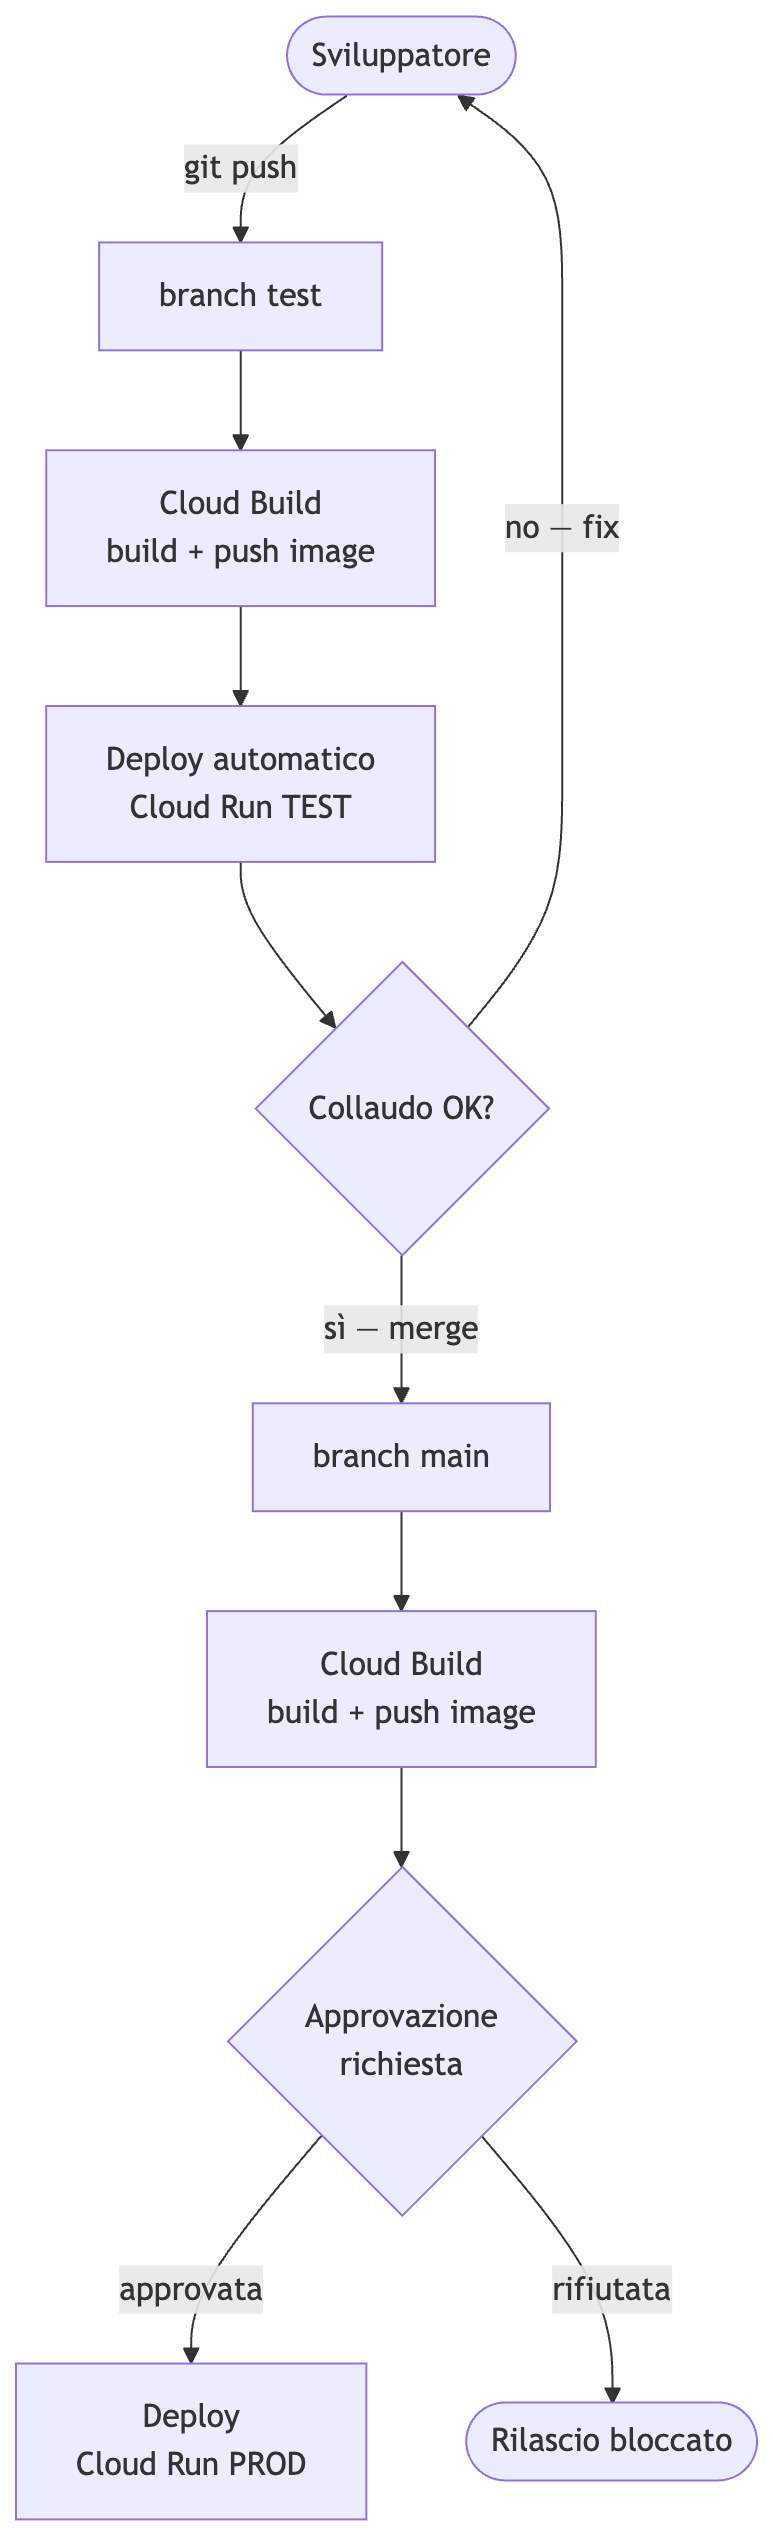
\includegraphics[height=0.75\textheight,keepaspectratio]{gitflow}
  \caption[Branching strategy e pipeline CI/CD]{La branching strategy adottata: ogni push sul branch \texttt{test} avvia un deploy automatico sull'ambiente di collaudo; il passaggio in produzione avviene tramite merge su \texttt{main} e richiede l'approvazione esplicita di un revisore prima del deploy su Cloud Run.}
  \label{fig:cicd_pipeline}
\end{figure}

\subsection{Identità, autenticazione e autorizzazione}
\label{subsec:agenti-auth}

L'autenticazione è interamente delegata a Microsoft Entra ID, che è l'unico
\emph{tenant} di identità usato in Cooperativa.
La scelta del flusso e della libreria segue lo standard di mercato per le \emph{single-page
applications}: il browser ottiene un \emph{access token} via
OAuth~2.0~\cite{rfc6749oauth2} e OpenID Connect~\cite{oidc1_0core} con
\emph{Authorization Code Flow + PKCE}, gestito dalla
\emph{Microsoft Authentication Library} (MSAL)~\cite{msft_msal} caricata nel
portale e nel pannello di amministrazione. Il token è un JWT firmato in
RS256~\cite{rfc7519jwt} ed è il vettore di autorizzazione che attraversa la
suite.

Sul lato server, la verifica del token Entra ID è affidata alla funzione
\texttt{verify\_entra\_token} all'atto del login federato ed esegue le verifiche
minime ma non negoziabili: scarica e mette in cache
le chiavi pubbliche da \texttt{JWKS} esposto da Microsoft, identifica la
chiave corretta tramite il campo \texttt{kid} dell'header, decodifica il
token con la libreria \texttt{python-jose} validandone audience e
firma e, infine, valida manualmente l'\texttt{issuer} contro la coppia
\texttt{(sts.windows.net, login.microsoftonline.com)}: questa
ridondanza è necessaria perché Entra ID emette token con \texttt{iss}
v1 o v2 a seconda dell'\emph{endpoint} usato, e l'opzione \texttt{verify\_iss}
del decoder accetta un solo valore alla volta. Una rotazione di chiavi non
prevista forza un secondo \emph{fetch} del JWKS prima di restituire un
errore 401: la cache non è quindi un \emph{single point of failure}.
Superata la verifica, il backend emette un JWT di sessione applicativo, firmato
con un segreto interno, che le richieste successive presentano alla dipendenza
FastAPI montata su ogni endpoint protetto. Accanto al login federato, un meccanismo
di autenticazione locale con credenziali dedicate resta riservato all'utenza
amministrativa di servizio (inizializzazione e accesso di emergenza).

L'autorizzazione si basa su un modello semplificato: un unico gruppo
Active Directory (``AI Users'') controlla l'accesso all'intera piattaforma.
Il claim JWT \texttt{group AI Users} contiene il GUID del gruppo;
il portale verifica la presenza dell'utente nel gruppo e, in caso positivo,
rende visibili gli agenti. I backend replicano la stessa verifica
sui propri endpoint. I claim
\texttt{preferred\_username}, \texttt{Ruolo} e \texttt{Direzione},
propagati dai sistemi HR a Entra ID, sono utilizzati per personalizzare
le risposte degli agenti (es. tono, contesto organizzativo) ma non per
controllare l'accesso.

Le Fig.~\ref{fig:login1} e~\ref{fig:login2} mostrano rispettivamente il punto di accesso al portale, da cui parte il flusso OAuth~2.0 + PKCE, e la schermata di autenticazione Entra ID personalizzata con il brand aziendale.

\begin{figure}[htbp]
  \centering
  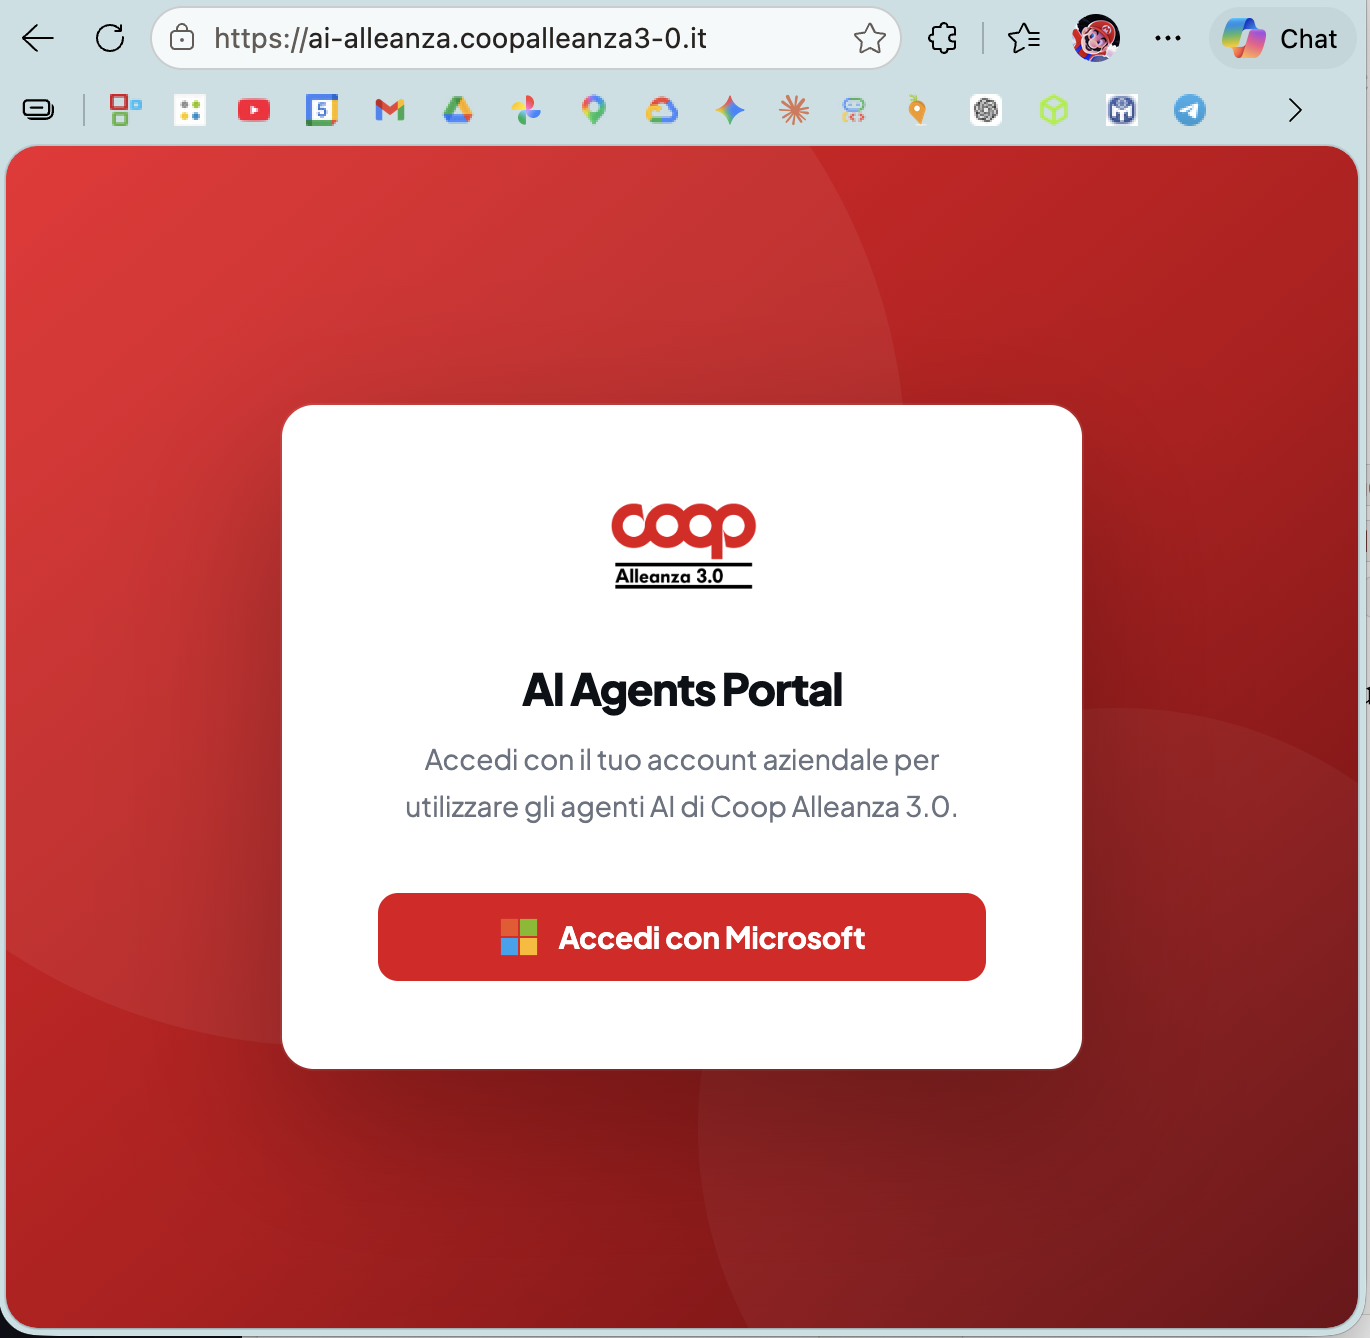
\includegraphics[width=0.75\textwidth,height=0.4\textheight,keepaspectratio]{login1}
  \caption[Portale agenti: pulsante di accesso]{Il portale agenti prima dell'autenticazione: il pulsante avvia il flusso OAuth~2.0 + PKCE delegato a Microsoft Entra ID tramite MSAL.}
  \label{fig:login1}
  \vspace{1em}
  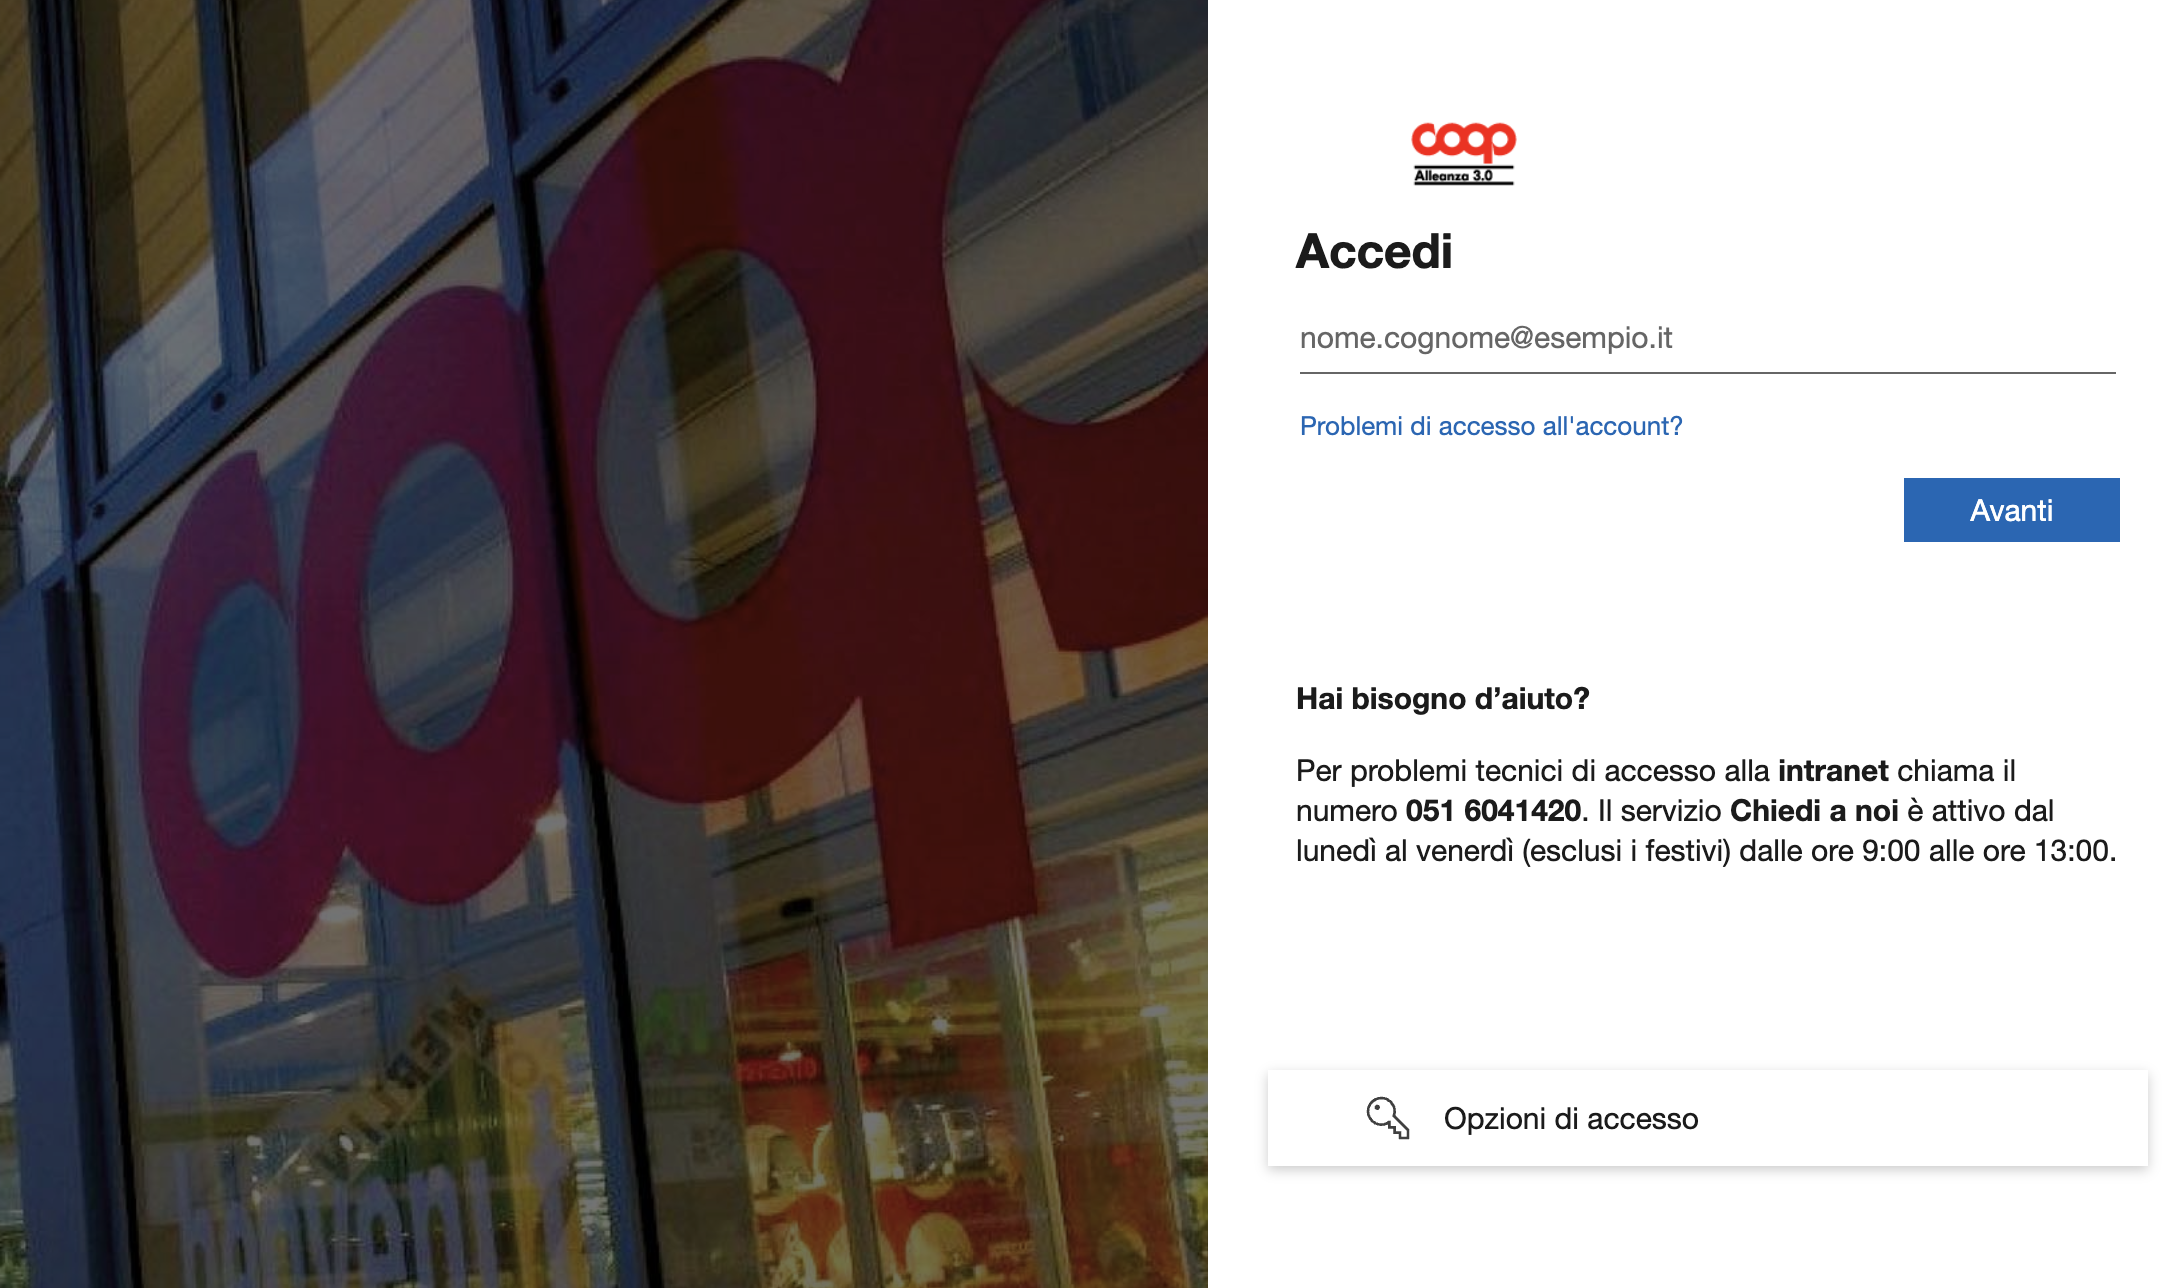
\includegraphics[width=0.75\textwidth,height=0.4\textheight,keepaspectratio]{login2}
  \caption[Schermata di autenticazione Microsoft personalizzata]{La schermata di autenticazione Microsoft Entra ID personalizzata con il brand dell'organizzazione:
  l'utente accede con le credenziali aziendali esistenti e controllo MFA, senza registrazione aggiuntiva.}
  \label{fig:login2}
\end{figure}

Il consumo di token è controllato da un servizio di quota su una \emph{tabella condivisa}
(\texttt{token\_budget}): ogni utente ha un budget mensile unico, indipendente dall'agente, su
fasce (\emph{Bronze}, \emph{Silver}, \emph{Gold}) modificabili dall'amministratore. Prima di ogni
chiamata il backend verifica il budget residuo e al termine contabilizza i token effettivi,
realizzando trasversalmente il principio di \emph{Implementazione agnostica e sostenibile}
(Sez.~\ref{sec:agenti-principi}).

Il prompt di sistema --- in ogni agente tranne CooPolicy, dove l'ottimizzazione avviene più a monte,
sul retrieval RAG --- impone una disciplina di output esplicita: ogni risposta apre con una sezione
\texttt{\#\#\# RAGIONAMENTO} (obiettivo, scelte, strategia), chiama i \emph{tool} appropriati e solo
dopo i risultati produce la sezione \texttt{\#\#\# RISPOSTA}. È una forma di Chain-of-Thought
esplicito~\cite{wei2022cot} con due tag che separano pianificazione e output; una funzione
\texttt{\_clean\_answer} collassa il blocco di ragionamento da quanto mostrato all'utente,
lasciandolo disponibile per l'auditing ma mantenendo pulita l'esperienza.

Le chiamate al modello sono racchiuse in un \texttt{try/except} che riconosce gli errori transitori
(\texttt{RESOURCE\_EXHAUSTED}, \texttt{429}, \texttt{503}, \emph{rate limit}) e li ripete con
\emph{backoff} lineare fino a tre tentativi, così che i picchi di traffico verso Vertex AI non
degradino il servizio percepito. La stessa strategia è usata da CooPolicy verso il RAG Engine e da
AllyCare e SysAid nelle query BigQuery.

% =====================================================================
\section{Il portale utente}
\label{sec:agenti-portal-impl}
% =====================================================================

Una volta autenticato, l'utente accede al portale (Fig.~\ref{fig:portal_menu}), che funge da punto di ingresso
unico per tutti gli agenti, in coerenza con il principio
di modularità verticale e accesso centralizzato
(Sez.~\ref{sec:agenti-principi}).

\begin{figure}[htbp]
  \centering
  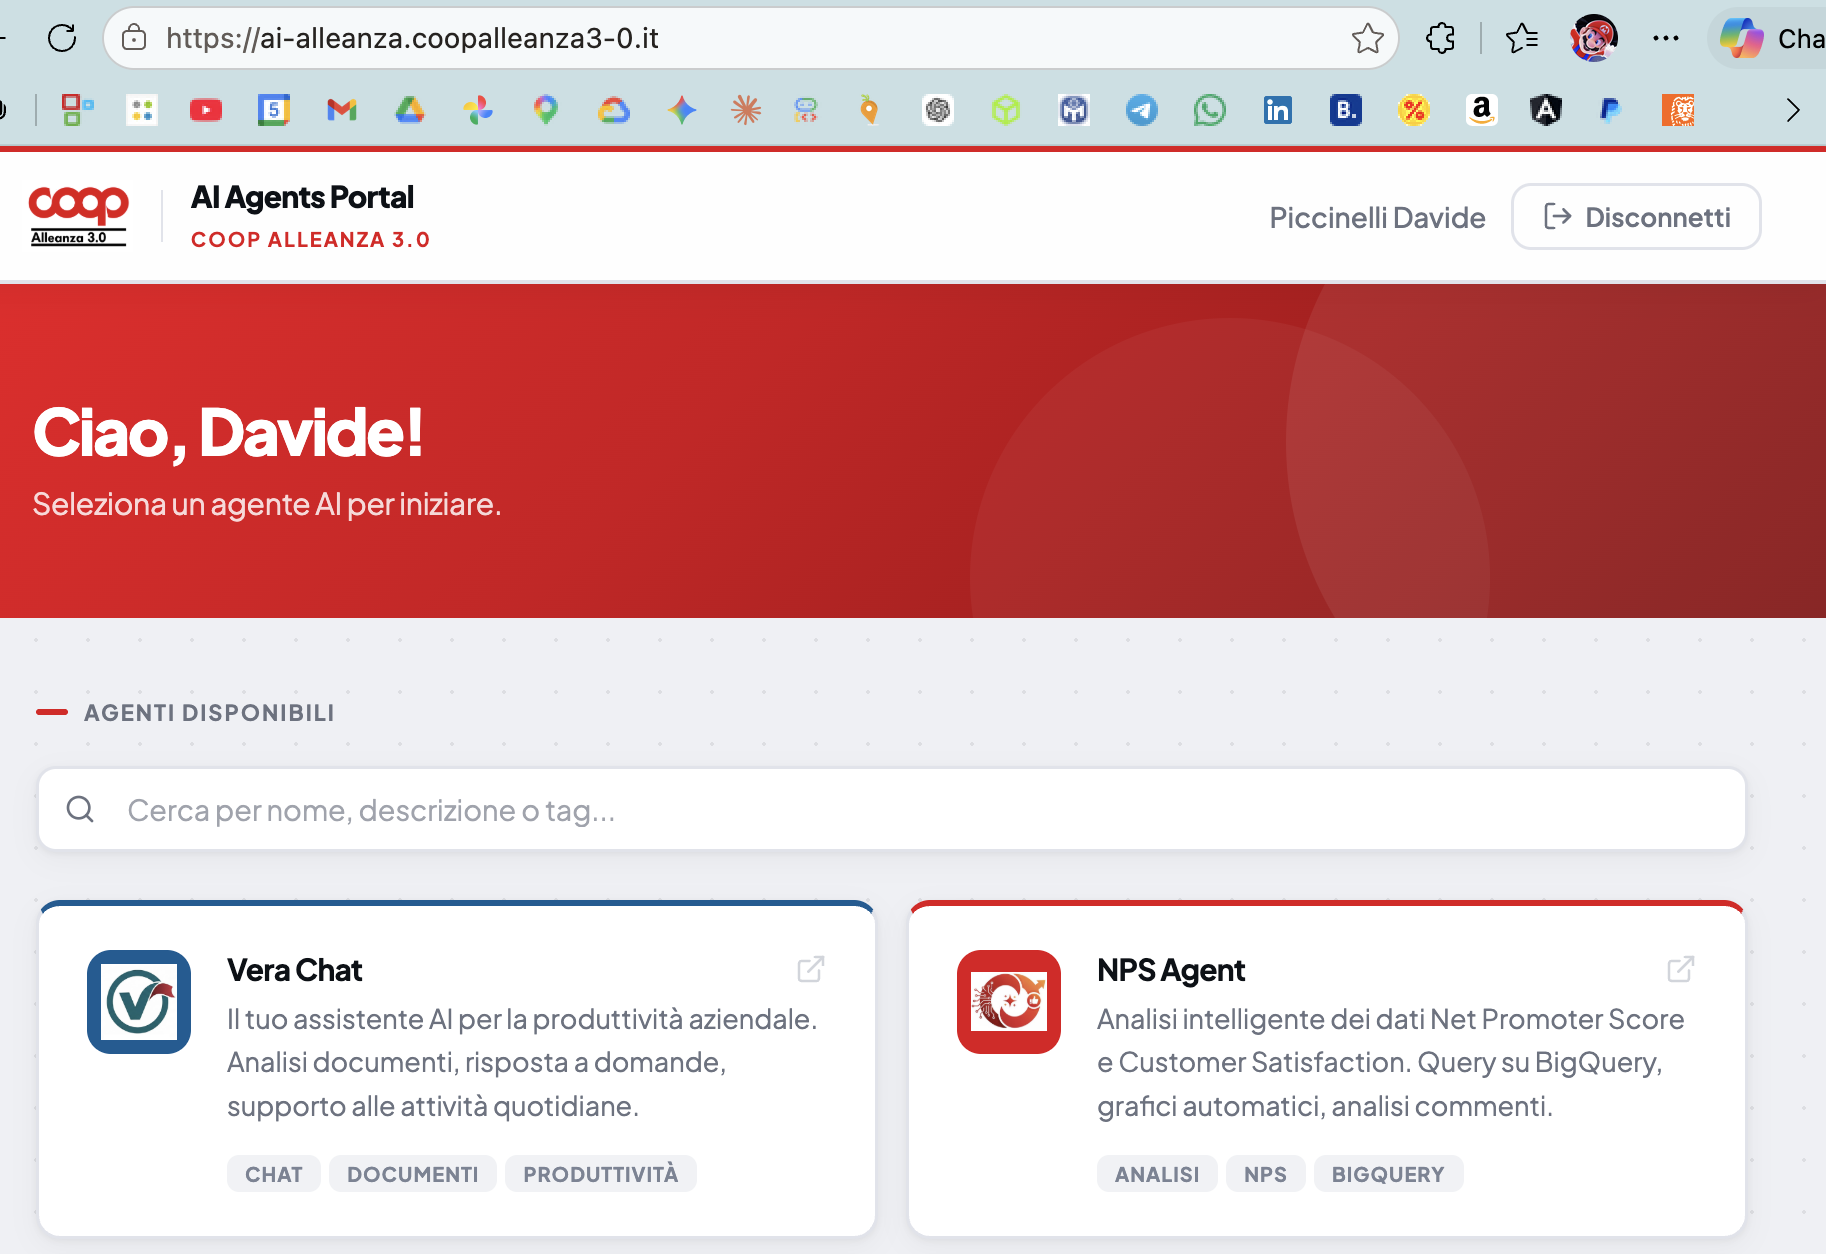
\includegraphics[width=0.9\textwidth,height=0.5\textheight,keepaspectratio]{portale}
  \caption[Menu di scelta degli agenti nel portale]{Il portale utente dopo il login: ogni agente è raggiungibile con un click senza ulteriori autenticazioni.}
  \label{fig:portal_menu}
\end{figure}
\FloatBarrier

% =====================================================================
\section{Vera --- assistente generale con Web grounding}
\label{sec:agenti-vera-arch}
% =====================================================================
\label{sec:agenti-vera-impl}

Vera è l'agente generalista della suite e il più articolato dal punto di
vista realizzativo: questa sezione ne presenta il caso d'uso e le scelte
implementative significative, che ruotano attorno a tre problemi:
\emph{routing} del modello, \emph{Web grounding} con citazioni inline,
gestione dei documenti caricati dall'utente.

\subsection{Caso d'uso e requisiti}
\label{subsec:vera-caso-uso}

Vera deve coprire i casi d'uso tipici di un LLM generalista (analisi e riassunto di documenti,
formazione, correzione di codice e formule e così via): supporta il caricamento di documenti via
RAG~\cite{lewis2020rag} nel maggior numero di formati e, per le richieste che richiedono
informazioni attuali, accede a internet via Web grounding~\cite{gcp_grounding}, ancorando la
generazione ai risultati di Google Search. La fonte, da documento o dal web, deve essere sempre
presente e verificabile, e va garantito che la ricerca non esfiltri i dati --- potenzialmente
confidenziali --- presenti nei documenti o nei prompt dell'utente.

\subsection{Routing del modello basato sulla complessità della query}
\label{subsec:vera-routing}

La selezione del modello è governata dal modulo \texttt{model\_router.py},
che stima la complessità della richiesta invocando Gemini~2.5 Flash con un
prompt di classificazione dedicato (\texttt{thinking\_budget = 0} per
minimizzare la latenza). La risposta è vincolata a una singola parola,
\texttt{low} o \texttt{high}, e determina se il turno sarà servito da
Flash (bassa complessità) o da Gemini~2.5 Pro (alta). Lo stesso schema di
classificazione è adottato da tutti gli agenti della suite (SysAid,
AllyCare, CooPolicy), garantendo un trade-off costo/qualità uniforme come
descritto nella Sez.~\ref{sec:bg-routing}.

\subsection{Pattern di esecuzione: documenti vs Web grounding}
\label{subsec:vera-paths}

Il generatore distingue due percorsi mutuamente esclusivi sulla base della
presenza di documenti caricati nella conversazione. Quando ci sono \emph{upload}
in stato \texttt{ready}, viene costruita o riusata una \emph{Gemini Context
Cache} associata alla conversazione, che evita di ricaricare i medesimi
documenti a ogni turno; la generazione avviene quindi tramite l'agente ADK
\texttt{doc\_qa\_agent}, configurato in modo da utilizzare la cache
(\texttt{generate\_content\_config.cached\_content}).
In assenza di upload, il generatore percorre il \emph{path} di conversazione
generale, che monta un \texttt{LlmAgent} ADK con
l'\texttt{EnterpriseWebSearchTool} integrato: il modello decide
autonomamente, in base alla domanda, se invocare la \emph{search} o
rispondere con la sola conoscenza parametrica.

In entrambi i percorsi la frammentazione dell'output è gestita con la modalità
\texttt{StreamingMode.SSE} di ADK: il \emph{loop} di eventi del Runner emette
\texttt{Event} parziali, di cui vengono propagate solo le \texttt{parts} con
campo \texttt{partial = True}, escludendo i blocchi marcati come
\texttt{thought}. Nel percorso di conversazione generale, quando il modello
restituisce \texttt{finish\_reason} uguale a \texttt{MAX\_TOKENS}, il backend
invia automaticamente un turno addizionale ``Continua la risposta dal punto
esatto in cui si è interrotta'' fino a una soglia di sicurezza
(\texttt{\_MAX\_CONTINUATIONS = 4}), così da rendere la risposta completa
anche quando supera il limite di output del modello.

\subsection{Citazioni inline e \emph{grounding metadata}}
\label{subsec:vera-citations}

Quando il modello invoca la \emph{Web search}, l'evento ADK porta in un campo
dedicato (\texttt{event.grounding\_metadata}) la lista dei chunk consultati,
con URL, titolo e \emph{snippet}. La funzione \texttt{extract\_web\_citations}
trasforma questa struttura in un array di citazioni che il frontend rende
inline, cliccabili dall'utente. Per i documenti caricati la citazione viene
estratta da un \texttt{citation\_extractor} che attraversa il testo finale e
risolve i riferimenti contro la lista dei \texttt{cache\_uploads}. Il fatto
che la fonte sia sempre verificabile e cliccabile, e che la sua presenza sia
imposta dal sistema (non opzionale per il modello), realizza il vincolo di
verificabilità descritto nella Sez.~\ref{subsec:vera-caso-uso}.

Le Fig.~\ref{fig:vera_conv_web} e~\ref{fig:vera_conv_doc} mostrano due conversazioni reali con Vera, rispettivamente in modalità Web grounding (con fonti citate inline) e dopo il caricamento di un documento.

\begin{figure}[htbp]
  \centering
  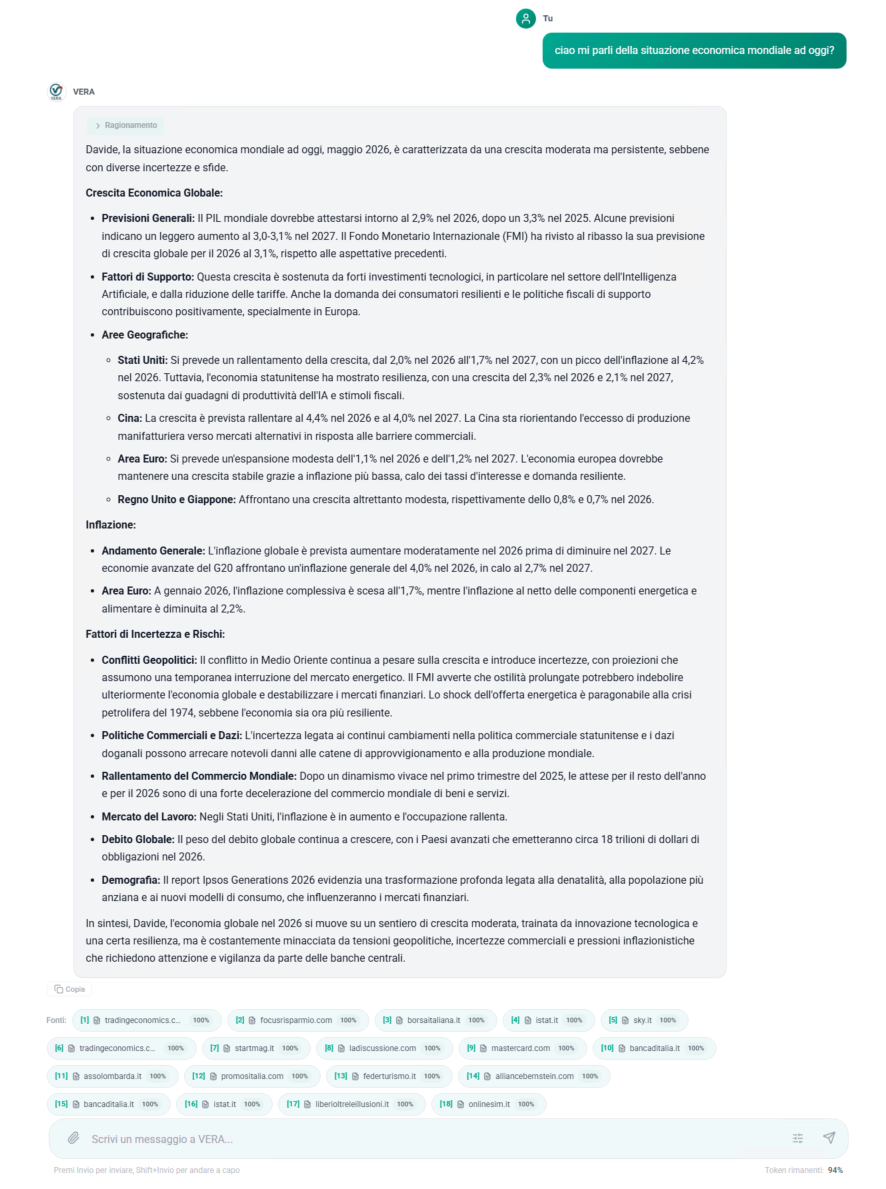
\includegraphics[width=0.68\textwidth,height=0.85\textheight,keepaspectratio]{vera1}
  \caption[Conversazione con Vera: Web grounding]{Una conversazione con Vera in modalità Web grounding: le fonti recuperate da Google Search sono citate inline e cliccabili dall'utente.}
  \label{fig:vera_conv_web}
\end{figure}

\begin{figure}[htbp]
  \centering
  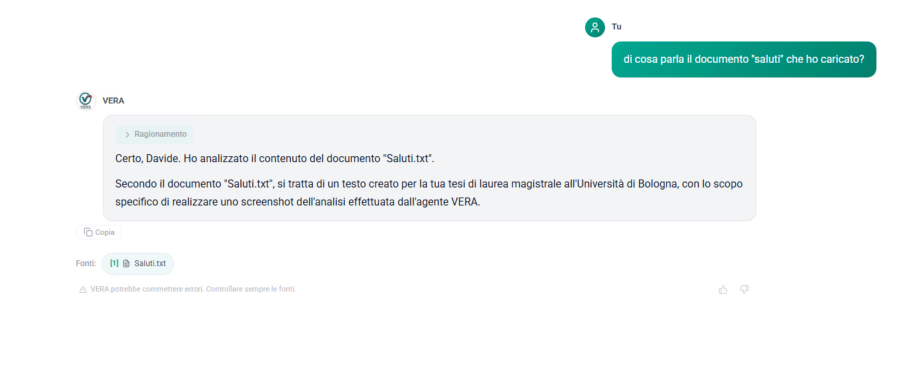
\includegraphics[width=\textwidth,keepaspectratio]{vera2}
  \caption[Conversazione con Vera: documento caricato]{Una conversazione con Vera dopo il caricamento di un documento: la risposta è ancorata al file tramite Gemini Context Cache e la fonte è indicata.}
  \label{fig:vera_conv_doc}
\end{figure}

\subsection{Catena di sicurezza pre e post generazione}
\label{subsec:agenti-security}

Coerentemente con il principio di governance facilitata, ogni invocazione di
modello in Vera attraversa una catena di controlli predisposta nel servizio
\texttt{model\_armor\_service.py}. La catena ha tre stadi:

\begin{enumerate}
  \item \textbf{Sanitizzazione del prompt.} Prima dell'invio all'LLM, il testo passa per il template
        di Google Cloud Model Armor~\cite{gcp_modelarmor} (Sez.~\ref{sec:bg-security}), che combina un classificatore
        \emph{Responsible AI} (\emph{hate}, \emph{harassment}, \emph{sexually explicit},
        \emph{dangerous}), il rilevatore di \emph{prompt injection}~\cite{perez2022promptinjection}
        e la \emph{Sensitive Data Protection}~\cite{gcp_dlp} per le PII, in linea con l'European AI
        Act~\cite{eu2024aiact}. Le PII del contesto italiano (Codice Fiscale, Partita IVA, IBAN) sono
        \emph{custom info types}; quando rilevate, il backend non maschera ciecamente il valore ma
        rifiuta la richiesta invitando a riformulare --- il \emph{tokenizing} cieco produrrebbe
        risposte inutilizzabili, poiché l'autenticità del dato è spesso necessaria.
  \item \textbf{Esenzioni per gruppo.} Alcuni gruppi (es. l'ufficio legale) hanno legittimo bisogno
        di trattare PII specifiche. Le tabelle \texttt{model\_armor\_group\_exemptions} e
        \texttt{pii\_group\_exemptions} consentono di escludere per gruppo singoli filtri o tipi di
        PII: alla verifica, il backend interseca le esenzioni attive dell'utente con i \emph{reasons}
        di Model Armor e, se ogni motivo è coperto, la richiesta prosegue.
  \item \textbf{Sanitizzazione della risposta e audit.} La stessa sanitizzazione si applica
        all'output prima del salvataggio, e ogni interazione è registrata in \texttt{chat\_logs}
        (action, modello, token in/out, flag citazioni). Gli eventi di blocco finiscono inoltre in un
        \emph{security log} dedicato che alimenta la dashboard di amministrazione
        (Sez.~\ref{sec:agenti-admin-impl}).
\end{enumerate}

\begin{figure}[htbp]
  \centering
  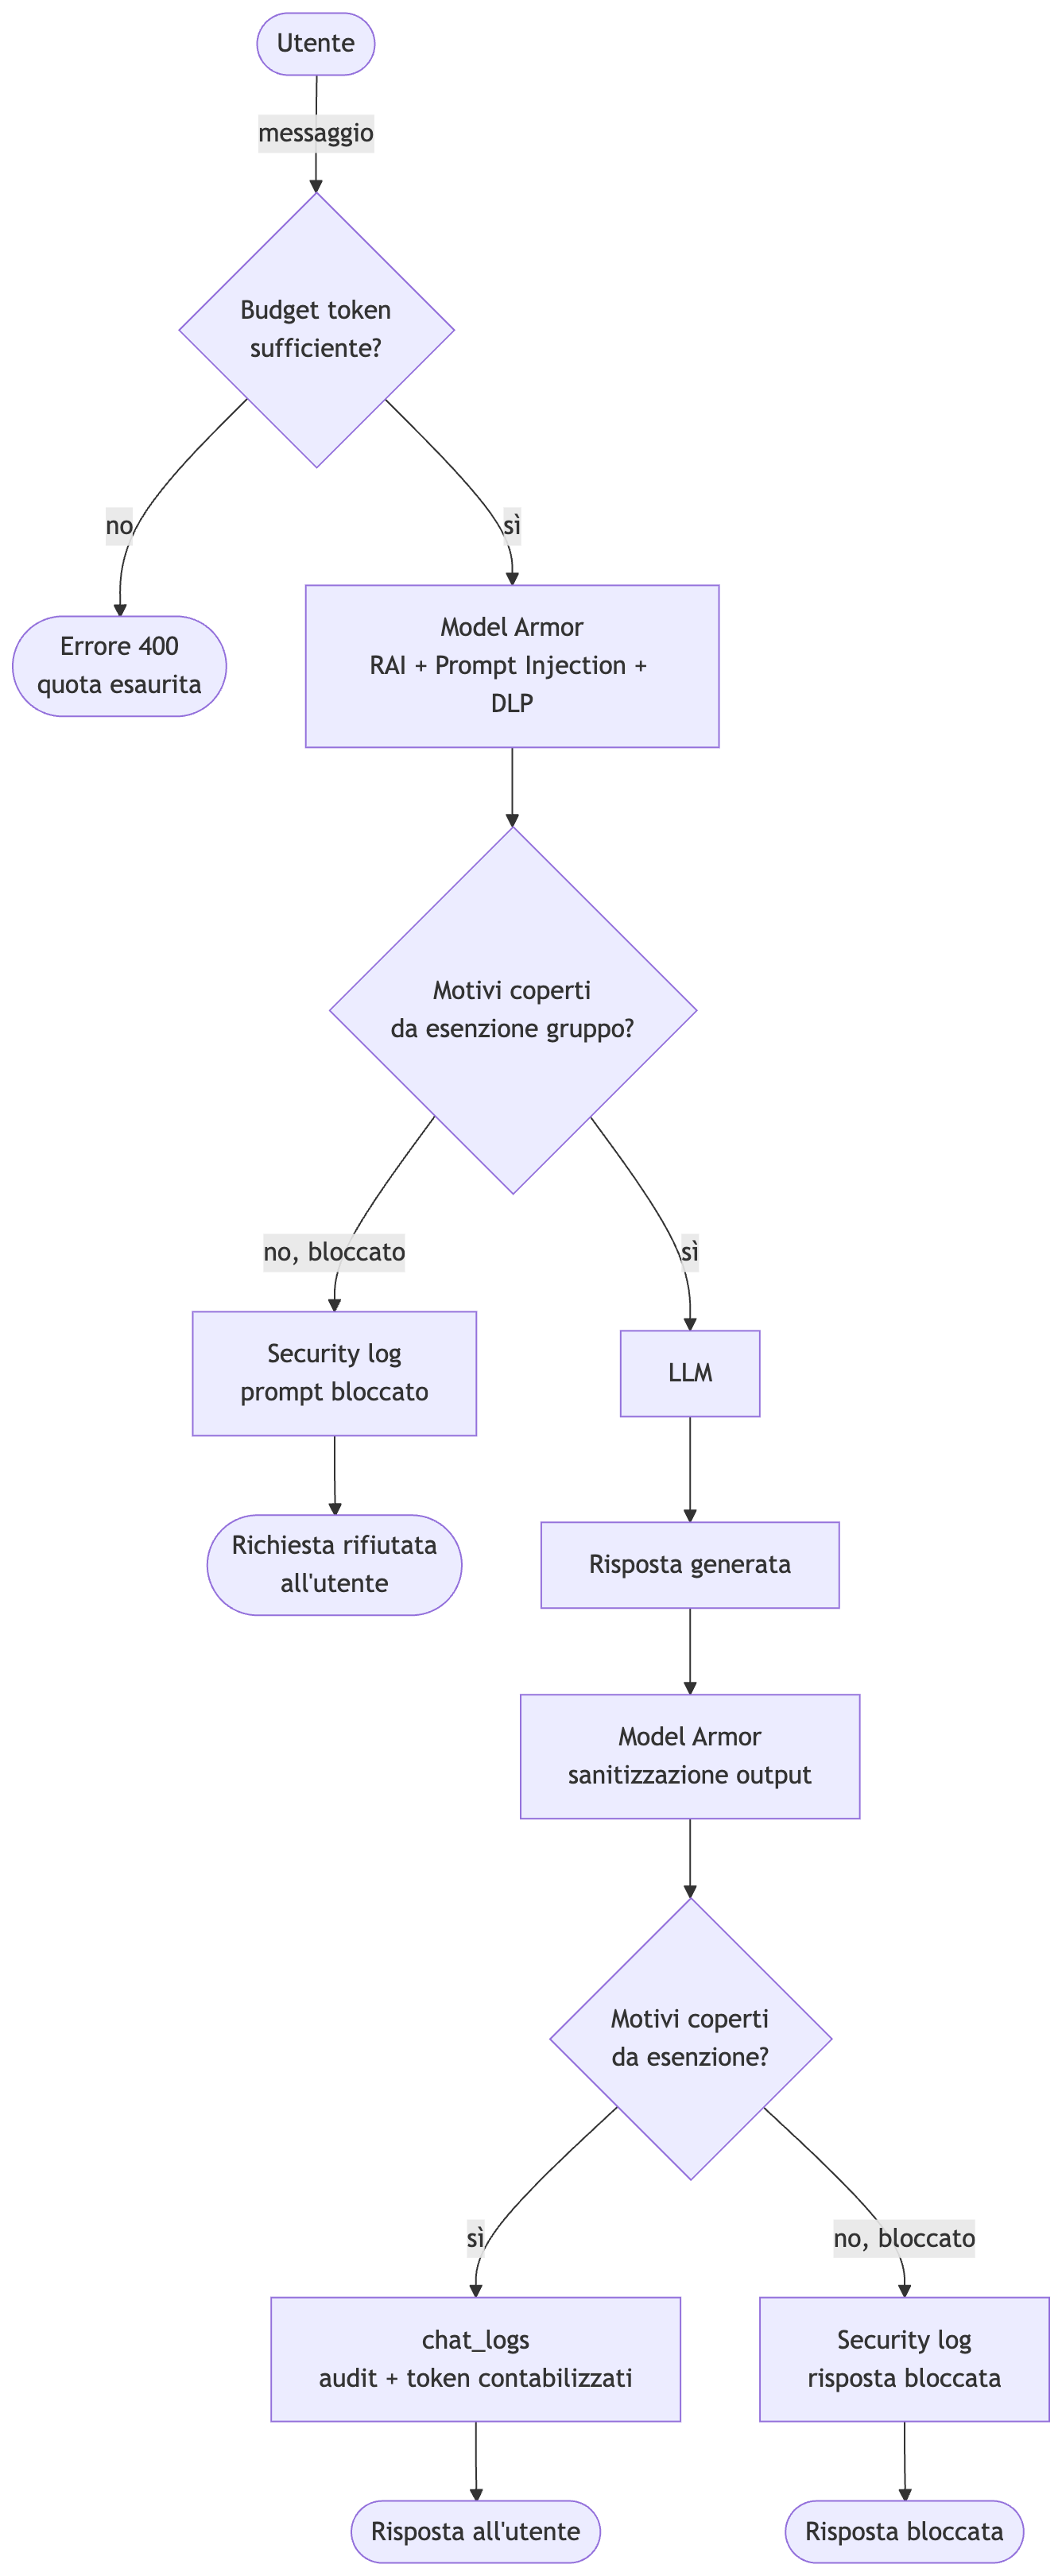
\includegraphics[width=0.85\textwidth,height=0.75\textheight,keepaspectratio]{flusso-prompt-full}
  \caption[Catena di sicurezza pre e post generazione]{Il flusso completo di una richiesta in Vera: verifica della quota, sanitizzazione del prompt tramite Model Armor
  (RAI + prompt injection + DLP) con gestione delle esenzioni per gruppo, chiamata al modello, sanitizzazione della risposta e
  audit su \texttt{chat\_logs}. Gli agenti verticali esclusivamente grounded non implementano questa catena (cfr.\ paragrafo successivo).}
  \label{fig:security_chain}
\end{figure}
\FloatBarrier

\paragraph{Ambito di applicazione.}
La catena è specifica di Vera; Orion (Cap.~\ref{chap:orion}) implementa la stessa, sanitizzando il
prompt prima di inoltrarlo ai sub-agenti. Gli altri agenti (SysAid, AllyCare, CooPolicy) non hanno
una propria catena pre/post generazione: in modalità \emph{standalone} operano solo sulla rete
interna con accesso autenticato (Sez.~\ref{subsec:agenti-auth}) e si affidano, come protezione a
livello di prompt, ai guardrail del proprio prompt di sistema (Sez.~\ref{sec:agenti-principi}).

% =====================================================================
\section{CooPolicy --- RAG su corpus di policy condiviso}
\label{sec:agenti-coopolicy-arch}
% =====================================================================
\label{sec:agenti-coopolicy-impl}

CooPolicy è la realizzazione ``RAG-native'' della suite: tutto il backend
ruota attorno alla pipeline di Retrieval-Augmented
Generation~\cite{lewis2020rag}, con scelte mirate a comprimere il rumore di
recupero e ad ancorare la generazione esclusivamente al materiale recuperato.

\subsection{Caso d'uso e requisiti}
\label{subsec:coopolicy-caso-uso}

L'agente è specializzato nella ricerca e interpretazione dei documenti normativi interni: gestisce
la documentazione della Intranet aziendale --- manuali, procedure, contratti di lavoro, organigrammi,
comunicazioni --- espansasi negli anni fino a diventare frastagliata e di non facile consultazione.

A differenza di Vera, CooPolicy non accede a fonti esterne: le risposte devono essere precise e
approfondite se il materiale è nel contesto RAG~\cite{lewis2020rag,guu2020realm}, oppure non essere
fornite affatto, sempre con fonti citate e accessibili. Per instradare anche richieste stringate, il
sistema classifica ogni query verso il corpus tematico più pertinente e applica una soglia di
rilevanza permissiva, delegando al modello la decisione finale sull'utilità dei chunk recuperati.

\subsection{Multi-corpus e classificazione della query}
\label{subsec:coopolicy-multicorpus}

Una prima scelta architetturalmente significativa è la rinuncia al
\emph{single corpus}. La documentazione interna è ripartita in dieci corpus
Vertex AI~\cite{gcp_vertex_rag} tematici (\texttt{policy-hr},
\texttt{contratti-smartworking}, \texttt{amministrazione-personale},
\texttt{procedure-aziendali}, \texttt{processi-regolamenti},
\texttt{governance-identita}, \texttt{sicurezza},
\texttt{punti-vendita-operativita}, \texttt{materiale-pdv},
\texttt{comunicazioni-generali}), ciascuno con un proprio descrittore in
italiano del dominio coperto. La motivazione è duplice: da un lato la
qualità del retrieval cala rapidamente al crescere della cardinalità dei
chunk indicizzati nello stesso spazio vettoriale; dall'altro, alcune
classi di documenti hanno regole di interpretazione
specifiche (i contratti collettivi vincolano la risposta in modo diverso
dalle policy aziendali) e mantenerle separate facilita l'evoluzione
indipendente e rende meno probabili ambiguità e risposte contraddittorie
o illogiche.

A monte del retrieval, una funzione \texttt{classify\_query} chiede a
Gemini~2.5 Flash di scegliere il \emph{corpus primario} ed eventualmente
un \emph{corpus secondario} fra quelli configurati, restituendo
strettamente un oggetto JSON con due chiavi. La scelta di Gemini Flash è
motivata dalla coppia di richieste essenziale di questo passo: bassa
latenza (sub-secondo) e basso costo unitario, condizione necessaria
perché il classificatore venga invocato a ogni richiesta senza pesare
sull'economia del sistema. Il prompt include il descrittore di ciascun
corpus disponibile.

\subsection{Retrieval e soglia di rilevanza}
\label{subsec:coopolicy-retrieval}

Il retrieval è eseguito in parallelo sui corpus selezionati attraverso
\texttt{rag.retrieval\_query} di Vertex AI RAG Engine~\cite{gcp_vertex_rag},
con \texttt{top\_k = 60} sul corpus primario e \texttt{top\_k = 30} sul
secondario quando presente. La ricerca è vettoriale densa: ogni query
viene trasformata in un embedding e confrontata per similarità coseno
con i vettori dei chunk indicizzati.

I chunk restituiti sono filtrati con una soglia
\texttt{RAG\_SCORE\_THRESHOLD~=~0.15} sulla distanza coseno: il valore è
permissivo, in coerenza con la decisione di delegare al
modello generativo (vincolato dal \emph{system prompt}) la decisione su
quali chunk siano effettivamente utili. L'aspettativa è che un modello in
modalità a bassa temperatura (Sez.~\ref{subsec:coopolicy-generation})
sappia rifiutare contesto irrilevante, mentre una soglia troppo restrittiva
rischia di escludere materiale marginalmente rilevante che però contiene
la risposta. I risultati di primario e secondario vengono uniti,
deduplicati per testo identico, ordinati per distanza coseno crescente
e troncati a \texttt{RAG\_TOP\_K} chunk totali.

\subsection{Arricchimento dei chunk e gestione dei metadati}
\label{subsec:coopolicy-meta}

Ogni PDF nel bucket GCS è accompagnato da un sidecar \texttt{.meta.json}
generato in fase di ingestione, contenente titolo leggibile e data del
documento. La funzione \texttt{\_enrich\_chunks\_with\_meta} scarica in
parallelo i sidecar dei chunk recuperati, con cache in-memory a TTL
un'ora, e arricchisce ciascun chunk con il titolo (dato che molti documenti avevano
nativamente nomi in esadecimale senza senso compiuto) e con la
data; quest'ultima è poi utilizzata dal modello per privilegiare la
fonte più recente in caso di ridondanza informativa. I file di metadati
(\texttt{.json}) e i tabulari grezzi (\texttt{.csv}), che possono
finire indicizzati per altri motivi, sono filtrati esplicitamente prima
di costruire il prompt, evitando che il modello citi rumore.

\subsection{Generazione vincolata e citazioni}
\label{subsec:coopolicy-generation}

Il prompt di sistema impone, in italiano, otto regole non negoziabili:
analisi integrale dei documenti recuperati prima di rispondere; risposta
basata esclusivamente sul materiale fornito; obbligatoriet\`a delle
citazioni \texttt{[N]} inline; massima precisione su numeri, articoli e
condizioni; divieto esplicito di parafrasi libere; tono professionale
italiano; consapevolezza temporale (preferire la fonte più recente,
avvisare se il documento ha più di due anni). Il modello è selezionato con
lo stesso classificatore di complessità descritto per Vera
(Sez.~\ref{subsec:vera-routing}): Gemini~2.5 Flash per richieste semplici,
Gemini~2.5 Pro per quelle complesse,
con \texttt{temperature = 0.1} e \texttt{max\_output\_tokens = 8192}. La
temperatura quasi zero massimizza l'aderenza al prompt e riduce
ulteriormente il rischio di allucinazione~\cite{xu2024hallucination}, in
linea con la funzione di un agente di tipo ``ricerca verificabile''.

Il post-processing della risposta è il dispositivo che garantisce
l'integrità delle citazioni. Le citazioni multiple
(\texttt{[1, 2, 3]}) vengono espanse in citazioni singole
(\texttt{[1][2][3]}); le citazioni con indice fuori dal range dei
documenti realmente forniti, se presenti,
vengono rimosse dal testo finale; gli indici sono infine rinumerati
in ordine di prima comparsa, in modo che la lista delle fonti
restituita al frontend rispecchi l'ordine di lettura. Per ciascuna
citazione viene anche estratto uno \emph{snippet} di 300~caratteri
centrato sulle keyword della query, utile per la \emph{preview} nel
frontend.

\subsection{ACL e proxy autenticato per i documenti}
\label{subsec:coopolicy-acl}

Il controllo di accesso avviene a monte, nel frontend orchestrato da
Orion: l'agente \texttt{coopolicy} è incluso nella lista degli agenti
disponibili solo per gli utenti che appartengono ad almeno un gruppo
Entra~ID presente nella \emph{whitelist} \texttt{DOCS\_ALLOWED\_GROUPS}.
Gli utenti non autorizzati non vedono l'agente e non possono quindi
raggiungerlo, eliminando la necessità di verifiche ridondanti a livello
di singolo endpoint. L'accesso al PDF originale, infine, non
avviene tramite URL pubblico: l'endpoint \texttt{/api/docs/file} agisce
come proxy autenticato che, verificato il token, ottiene un \emph{access
token} cloud-platform tramite le credenziali del service account del
servizio e scarica il binario direttamente dall'API di GCS, restituendolo
con \texttt{Content-Disposition: inline}. Il modello non ha mai
visibilit\`a degli URL firmati e l'utente non pu\`o aggirare la
verifica del token visitando un link.

Le Fig.~\ref{fig:coopolicy_conv1} e~\ref{fig:coopolicy_conv2} mostrano una conversazione con CooPolicy e il relativo pannello delle fonti, da cui il PDF originale è raggiungibile attraverso il proxy autenticato appena descritto.

\begin{figure}[htbp]
  \centering
  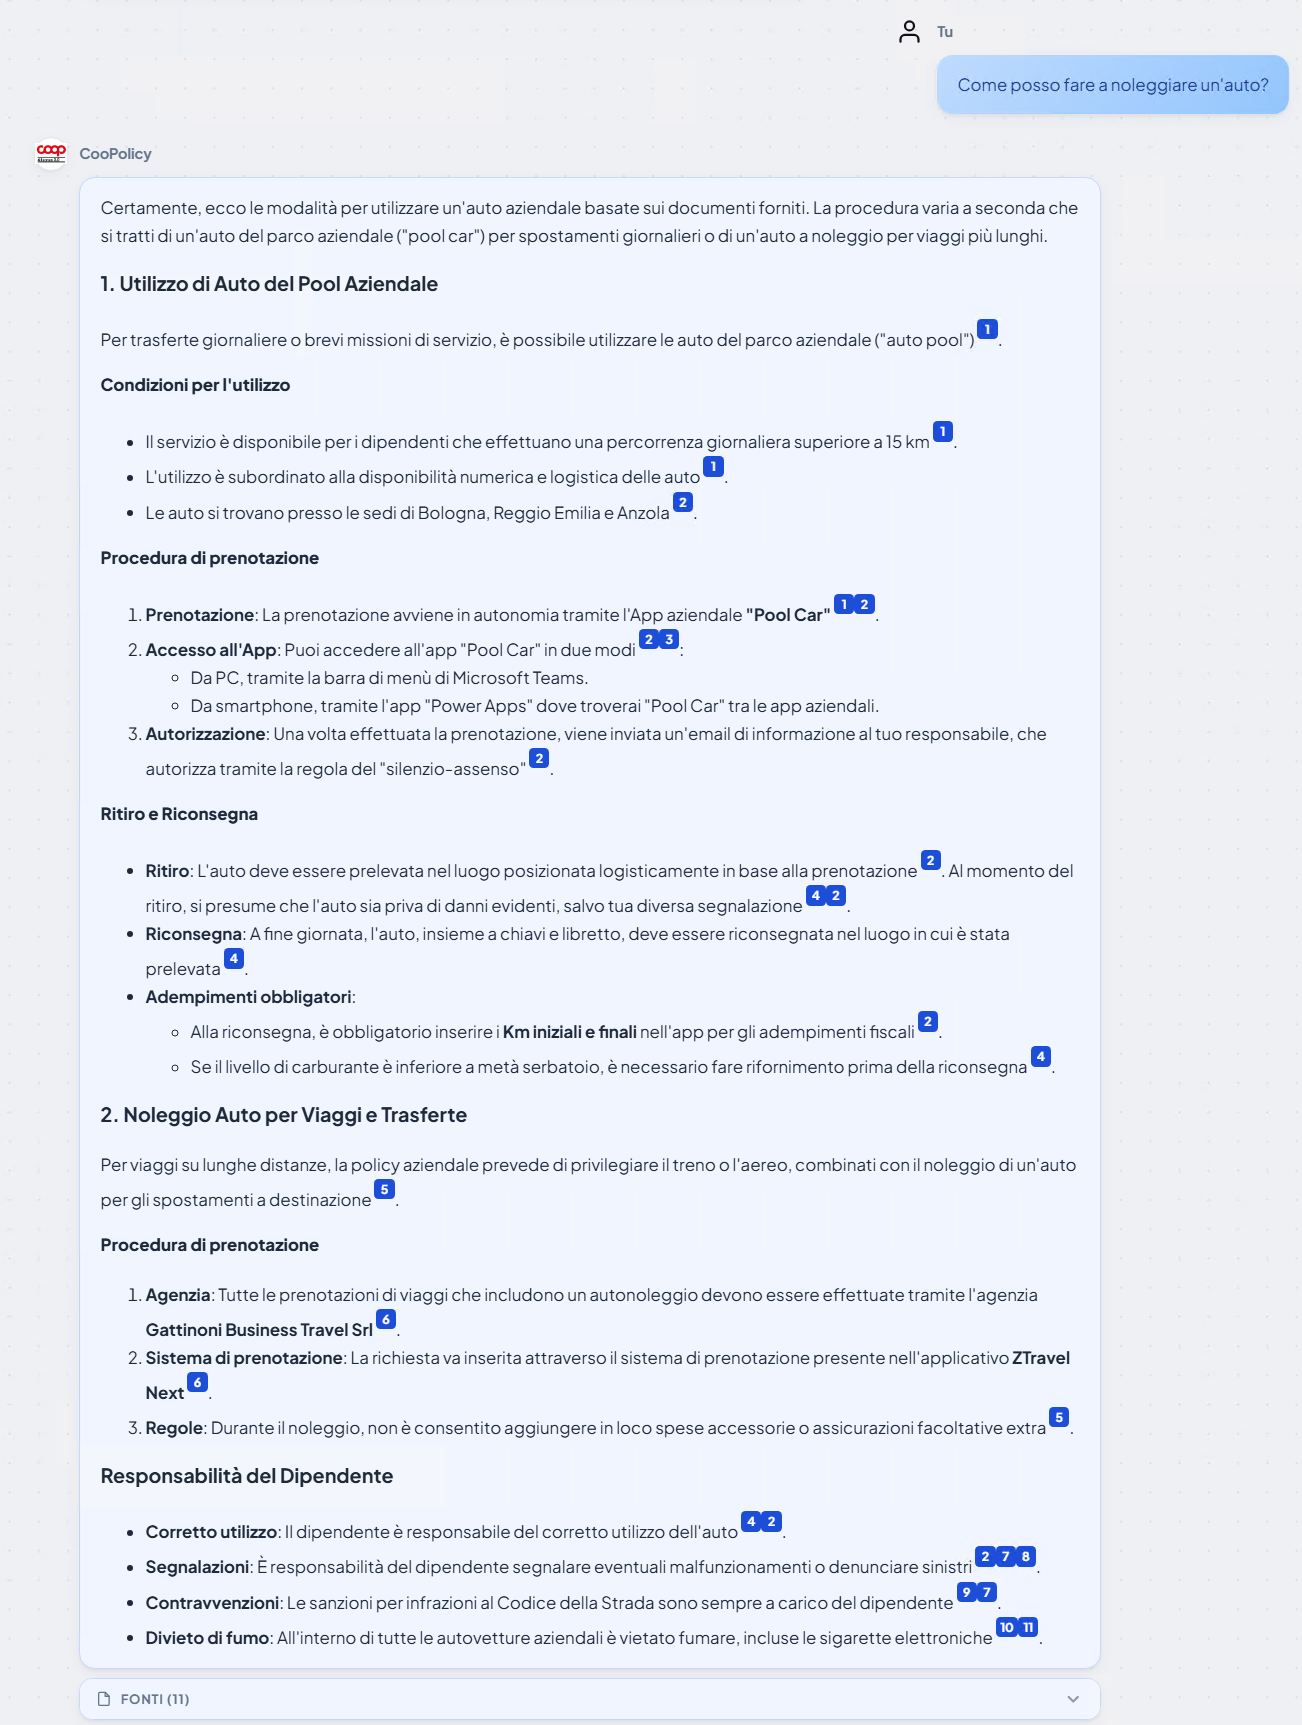
\includegraphics[width=0.68\textwidth,height=0.85\textheight,keepaspectratio]{coopolicy2}
  \caption[Conversazione con CooPolicy: risposta da corpus policy]{Una conversazione con CooPolicy: la risposta è basata esclusivamente sui documenti del corpus RAG,
  con citazioni numerate \texttt{[N]} che rimandano alla fonte originale.}
  \label{fig:coopolicy_conv1}
\end{figure}

\begin{figure}[htbp]
  \centering
  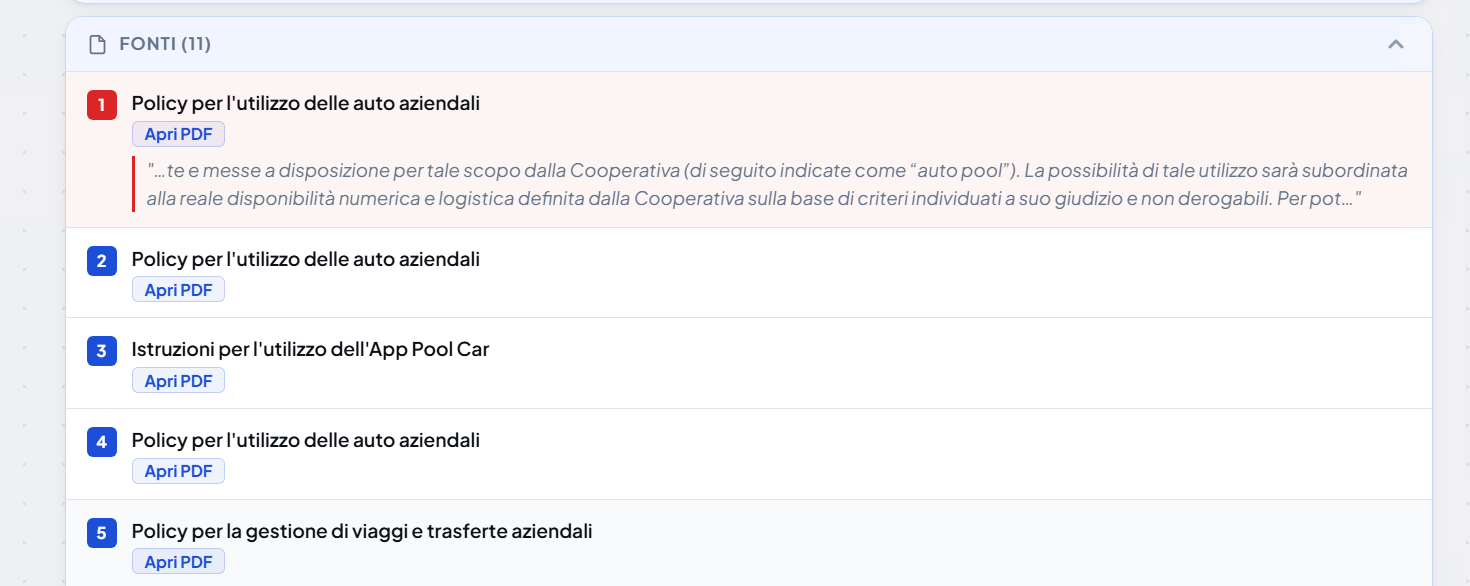
\includegraphics[width=0.95\textwidth,keepaspectratio]{coopolicy3}
  \caption[Pannello delle fonti di CooPolicy]{Il pannello delle fonti restituito da CooPolicy: ogni citazione numerata rimanda al documento originale,
  accessibile tramite il pulsante ``Apri PDF'' servito dal proxy autenticato verso GCS (Sez.~\ref{subsec:coopolicy-acl}).}
  \label{fig:coopolicy_conv2}
\end{figure}

% =====================================================================
\section{AllyCare / NPS --- Text-to-SQL sui dati dei sondaggi}
\label{sec:agenti-allycare-arch}
% =====================================================================
\label{sec:agenti-allycare-impl}

AllyCare è la realizzazione del paradigma Text-to-SQL
(Sez.~\ref{subsec:bg-text2sql}) su BigQuery per l'analisi dei sondaggi NPS.
L'implementazione espone al modello tre \emph{tool} di interazione con i
dati e affida all'\emph{agentic loop} di ADK la gestione del ciclo ReAct
(Sez.~\ref{sec:bg-multiagent}).

\subsection{Caso d'uso e requisiti}
\label{subsec:allycare-caso-uso}

L'agente è specializzato nell'analisi dei sondaggi NPS (Net Promoter Score) dell'organizzazione. La
base dati tabellare, in aggiornamento costante, raccoglie per ogni sondaggio i voti sui vari aspetti
dell'esperienza d'acquisto più un campo di testo libero; un flusso LLM dedicato analizza i commenti
e li cataloga (reparto, argomento, sentiment), producendo una tabella ``ai enriched'' che affianca ai
dati di base i tag generati.

AllyCare facilita le analisi su questa tabella, coprendo sia compiti da reportistica ad hoc (domande
quantitative come ``voti positivi nel periodo X per il negozio Y'', grafici di andamento) sia analisi
qualitative onerose (``elenca le maggiori criticità in una regione/negozio''). La richiesta è tradotta
dal modello in una o più query SQL, eseguite e usate per la risposta e le analisi successive.

\subsection{Iniezione selettiva dello schema}
\label{subsec:allycare-schema}

Il prompt di sistema include lo schema BigQuery delle due tabelle
rilevanti (\texttt{mapp\_nps\_survey\_internal\_prod} con i dati di
sondaggio grezzi e \texttt{mapp\_nps\_survey\_ai\_enriched\_prod} con i
campi prodotti da una pipeline di arricchimento AI a monte) ottenuto via
\texttt{bq\_client.get\_table} e mantenuto in cache per un'ora. Allo
schema tecnico viene affiancato un \emph{glossario semantico} in
italiano: per ciascuna colonna è descritto il significato funzionale
(es. \texttt{voto\_item01: ``Il personale del negozio è gentile e
competente''; valori -2 = mancata risposta, -1 = non lo so, 0--9 = voto}).
Insieme allo schema viene iniettata anche la lista esatta delle
descrizioni di negozio (\texttt{store\_desc}, in cache 24~ore) tratta
direttamente da BigQuery, in modo che il modello possa risolvere
varianti colloquiali (``Sasso'', ``Iper Bologna'') in match esatti senza
allucinare codici. Questa strategia di \emph{schema injection
selettiva}, in luogo dell'esposizione del catalogo completo del data
warehouse, è coerente con la letteratura
Text-to-SQL~\cite{pourreza2023dinsql}: meno colonne il modello vede,
meno opportunità ha di confondersi.

Il prompt impone inoltre regole di consistenza SQL specifiche del
dominio: i filtri sui voto-item devono includere \texttt{voto\_itemXX
>= 0} nella \texttt{WHERE} (escludendo i marcatori \texttt{-1} e
\texttt{-2}); tutti i confronti su campi categorici testuali devono
usare \texttt{UPPER(TRIM(...))} per neutralizzare incoerenze di
\emph{case}; la distinzione fra \texttt{LIKE} e uguaglianza esatta
sui nomi di negozio segue regole esplicite. L'effetto è che AllyCare
tipicamente non sbaglia i filtri ``stupidi'' che dominano gli errori in
Text-to-SQL applicato in dominio reale.

\subsection{I \emph{tool} disponibili l'\emph{agentic loop} ADK}
\label{subsec:allycare-tools}

Lo strato di tool è dichiarato in \texttt{tools.py} ed esporta tre
funzioni Python registrate come \emph{ADK tools}:

\begin{description}
  \item[\texttt{run\_sql(query)}]
    Esegue una query SQL su BigQuery con un \emph{guard} sintattico: la
    query è parsificata con \texttt{sqlparse} e respinta se contiene
    \texttt{DDL} o \texttt{DML} di scrittura
    (\texttt{INSERT}/\texttt{UPDATE}/\texttt{DELETE}); se non già
    presente, viene aggiunto un \texttt{LIMIT~5000}; il job è eseguito
    con \texttt{maximum\_bytes\_billed = 10\textsuperscript{9}} per
    bloccare query accidentalmente costose. Il risultato è restituito
    al modello come tabella Markdown delle prime 750~righe, con
    indicazione del totale; la copia completa del DataFrame è
    memorizzata nello \texttt{tool\_context.state} per essere
    riutilizzata da \texttt{generate\_chart} senza una seconda
    interrogazione. Se la query produce un errore SQL, il messaggio
    viene impacchettato come \texttt{function\_response} e il modello
    può auto-correggersi al ciclo successivo: questo è il meccanismo
    concreto di \emph{self-correction}~\cite{pourreza2023dinsql}.
  \item[\texttt{analyze\_comments(query, question)}]
    Estrae un campione di commenti testuali grezzi mediante una query
    dedicata, ne preleva un sotto-campione casuale di al più 200 record
    e chiede a Gemini~2.5 Pro una sintesi qualitativa con citazioni
    \emph{verbatim}. Il prompt di analisi è scritto in modo da essere
    integrato nella risposta più ampia e da non duplicare l'intestazione
    di sezione. È usato esclusivamente per analisi qualitative: per
    qualunque dato quantitativo (sentiment, conteggi di temi, percentuali)
    il prompt di sistema impone \texttt{run\_sql} sulla tabella
    \texttt{ai\_enriched\_prod}.
  \item[\texttt{generate\_chart(visualization\_goal)}]
    Costruisce un grafico Matplotlib/Seaborn a partire dal DataFrame
    cachato dall'ultimo \texttt{run\_sql}, scegliendo la rappresentazione
    in funzione di parole-chiave nel \emph{goal}
    (\texttt{torta}/\texttt{pie} $\rightarrow$ pie chart;
    \texttt{linee}/\texttt{trend} $\rightarrow$ line chart; default
    $\rightarrow$ bar chart). Il grafico è codificato in PNG, convertito
    in base64 con prefisso \emph{data URI} e iniettato nel session state.
    Il backend lo restituisce poi nella risposta come campo
    \texttt{chart\_and\_data}, lasciando il rendering alla logica del
    frontend. Il chart viene incluso nel payload finale solo se
    \texttt{generate\_chart} è stato effettivamente invocato nel turno,
    evitando di restituire il grafico del turno precedente.
\end{description}

L'\emph{agentic loop} è governato dal \texttt{Runner} ADK che, a partire
dall'\texttt{LlmAgent} configurato con i tre tool e con il prompt di
sistema, alterna in modo trasparente fasi di ragionamento e chiamate a
tool fino a quando il modello restituisce la risposta finale. Il
modello scelto per il turno (Pro o Flash) è iniettato nell'agente al
momento della costruzione, e il prompt di sistema include il nome
proprio dell'utente e la sua direzione (estratti dal token Entra ID),
così che il tono della risposta sia personalizzato.

La selezione del modello segue lo stesso schema adottato per SysAid
(Sez.~\ref{subsec:sysaid-arch-unificata}): il campo \texttt{complexity}
propagato da Orion determina se il turno è servito da Gemini~2.5 Flash
(\texttt{low}) o Gemini~2.5 Pro (\texttt{high}). Quando AllyCare è
usato in modalità standalone, la complessità è stimata localmente dal
modello Flash con una chiamata di classificazione dedicata,
coerentemente con il pattern già descritto per SysAid.

\subsection{Disciplina del ragionamento, anti-allucinazione}
\label{subsec:allycare-discipline}

La ``gerarchia della verità'' codificata nel prompt impone che i dati
del database siano la sola fonte autoritativa: il modello non può
classificare commenti per produrre numeri (la categorizzazione
quantitativa va sempre dalla tabella arricchita). Una regola di
``fiducia nel tool'' impone inoltre che, se \texttt{run\_sql} ha
restituito un dato, sia quel dato a essere riportato, anche se il
modello ``ricorda'' numeri diversi da turni precedenti.

Le Fig.~\ref{fig:allycare_conv1}, \ref{fig:allycare_chart} e~\ref{fig:allycare_conv2} mostrano tre interazioni con AllyCare: un'analisi quantitativa dell'NPS, un grafico generato dinamicamente dai dati estratti via SQL e un'analisi qualitativa dei commenti liberi.

\begin{figure}[htbp]
  \centering
  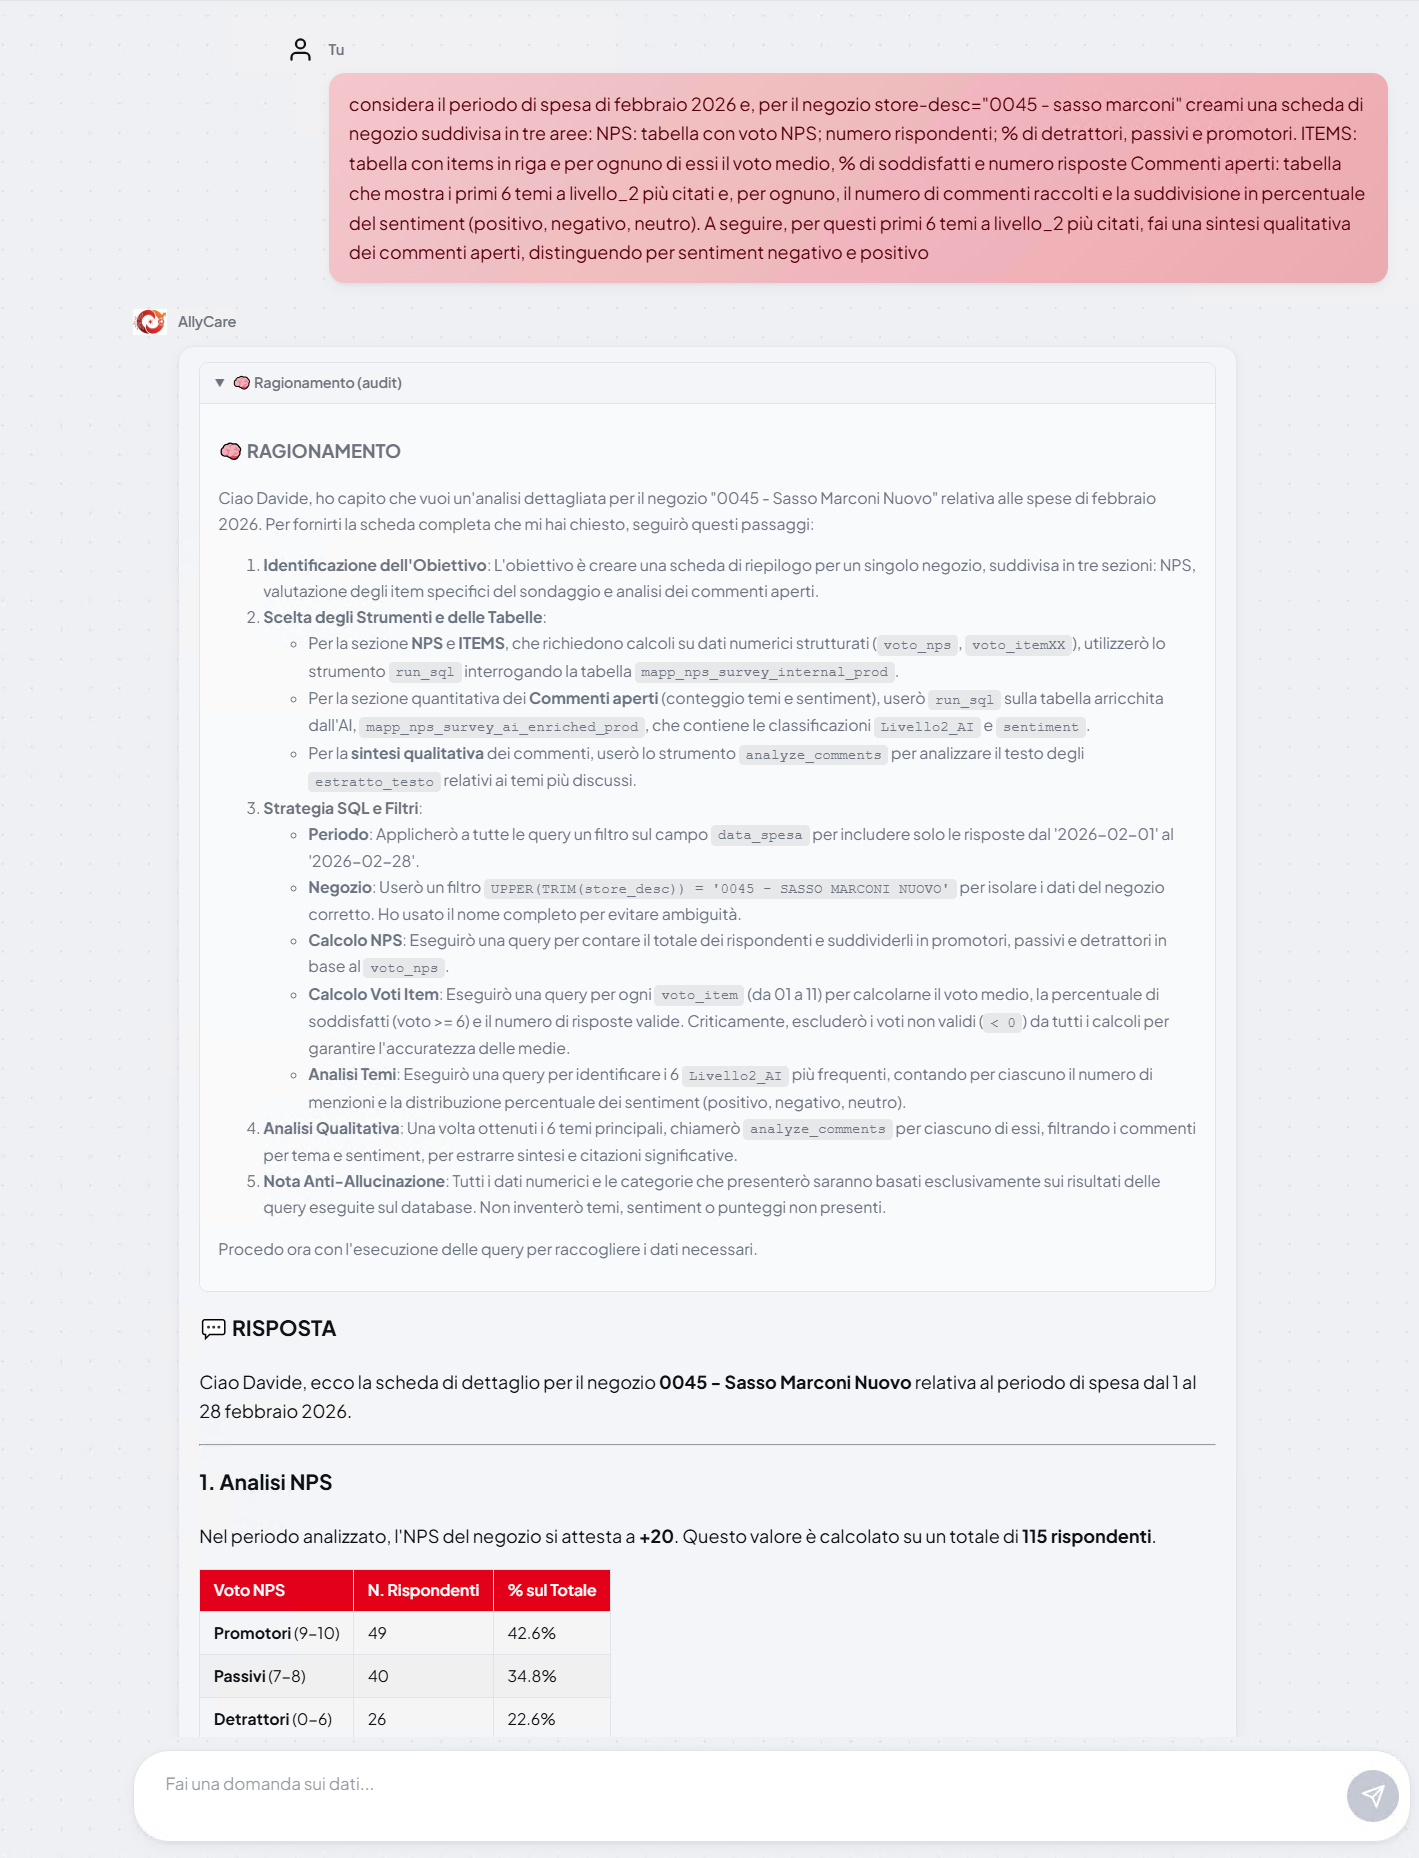
\includegraphics[width=0.68\textwidth,height=0.85\textheight,keepaspectratio]{nps2}
  \caption[Conversazione con AllyCare: analisi quantitativa]{Una conversazione con AllyCare: la richiesta di analisi NPS produce una sezione di \emph{ragionamento}
  esplicito (con la strategia SQL adottata) seguita da una risposta numerica strutturata (punteggio NPS, suddivisione promotori/passivi/detrattori).}
  \label{fig:allycare_conv1}
\end{figure}

\begin{figure}[htbp]
  \centering
  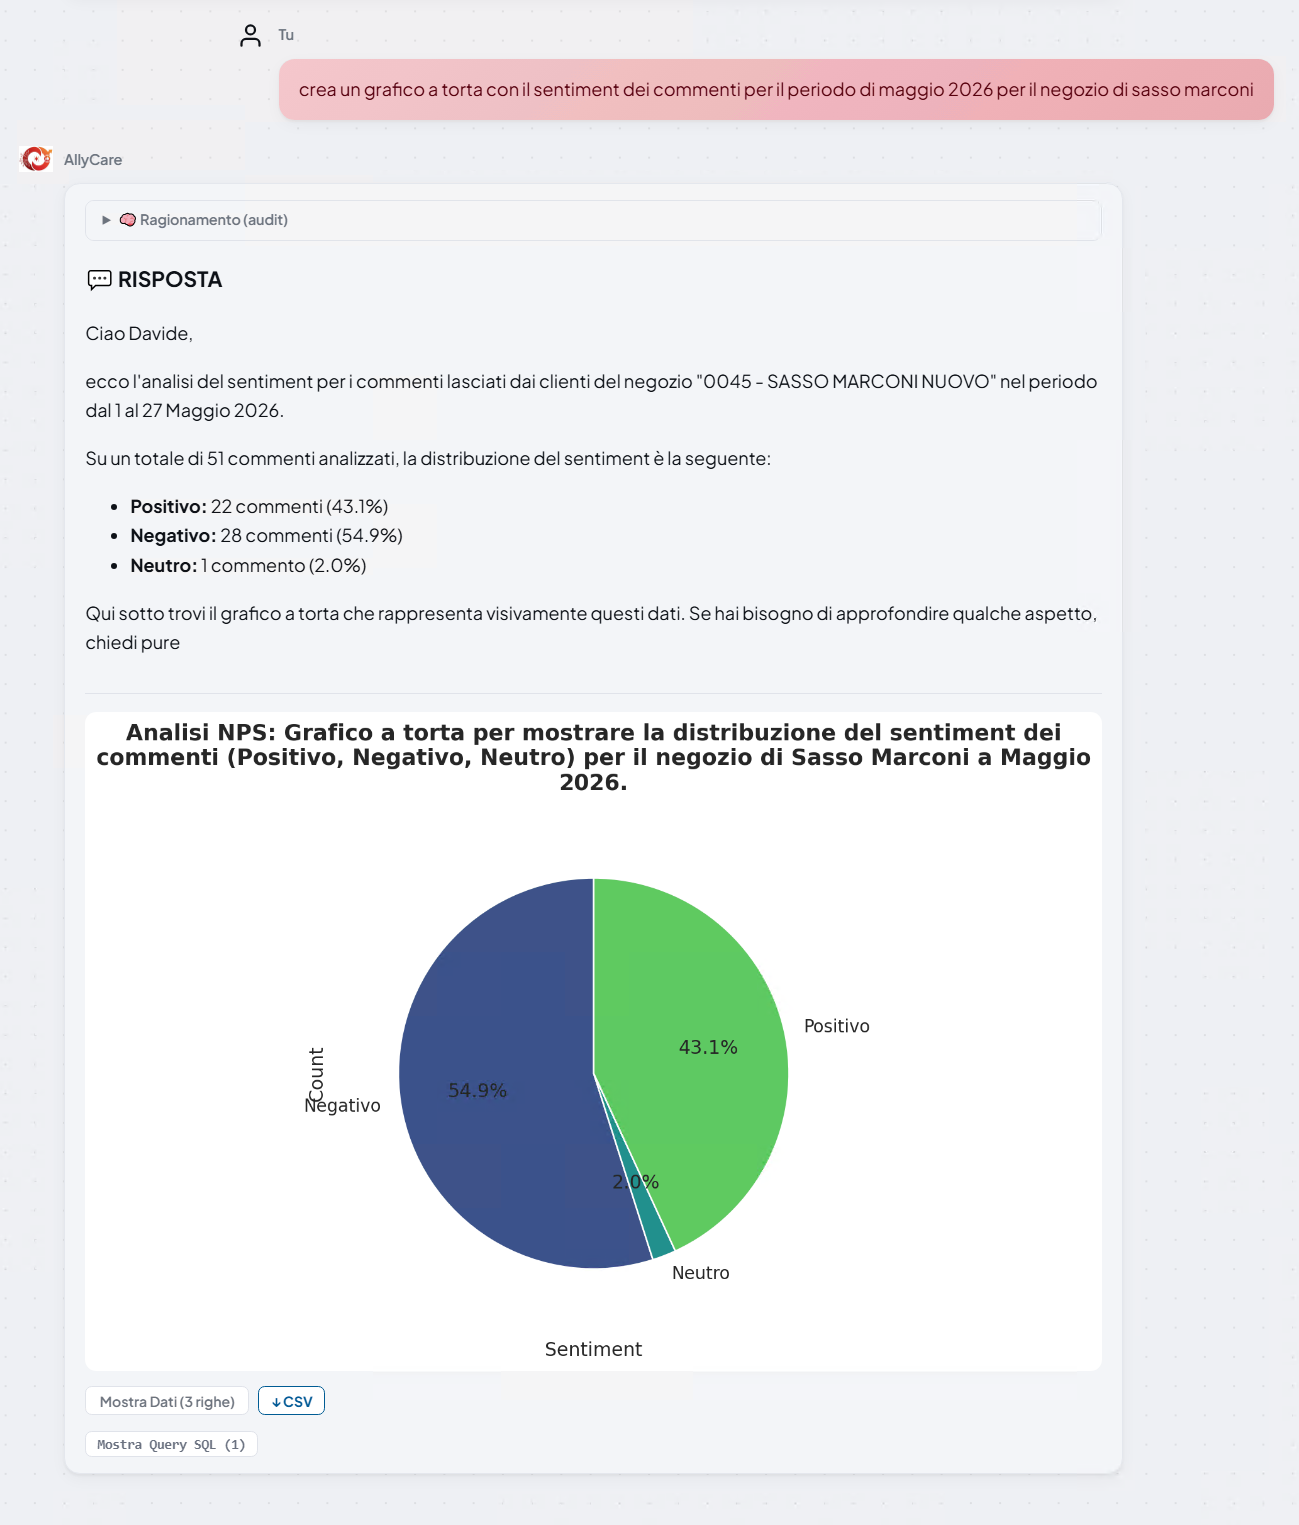
\includegraphics[width=0.6\textwidth,height=0.8\textheight,keepaspectratio]{nps5}
  \caption[AllyCare: grafico generato dinamicamente]{AllyCare genera dinamicamente un grafico (qui un grafico a torta della distribuzione del \emph{sentiment} dei commenti) a
  partire dai dati estratti via SQL, codificandolo come immagine restituita al frontend.}
  \label{fig:allycare_chart}
\end{figure}

\begin{figure}[htbp]
  \centering
  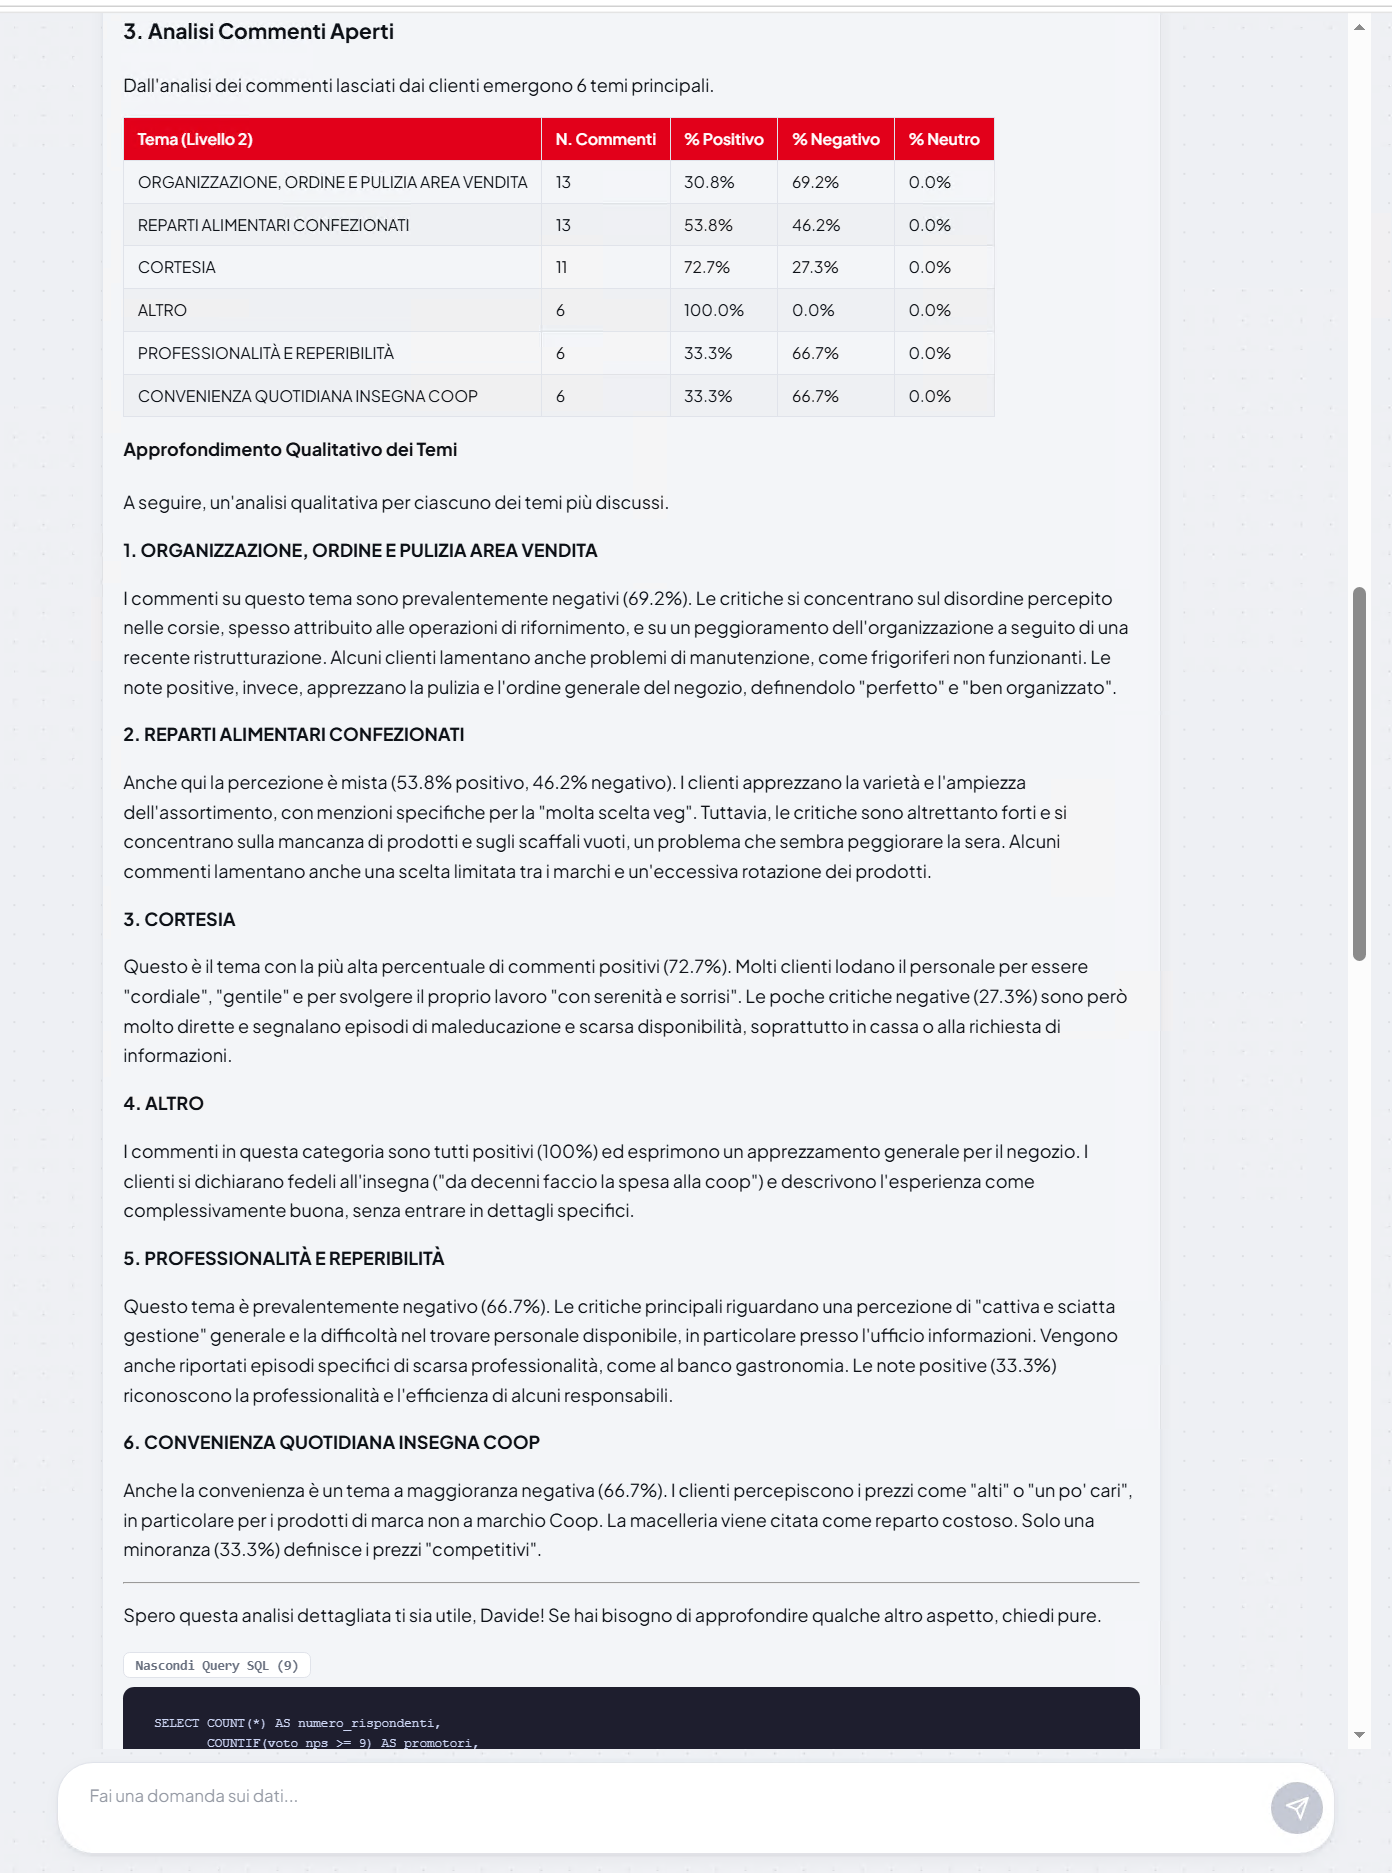
\includegraphics[width=0.68\textwidth,height=0.85\textheight,keepaspectratio]{nps4}
  \caption[Conversazione con AllyCare: analisi qualitativa dei commenti]{AllyCare in modalità analisi qualitativa: i commenti testuali liberi del sondaggio sono sintetizzati per tema,
  con la relativa distribuzione di \emph{sentiment}, senza produrre numeri non supportati dalla tabella arricchita.}
  \label{fig:allycare_conv2}
\end{figure}

% =====================================================================
\section{SysAid --- Text-to-SQL sul ticketing con modelli LLM distinti}
\label{sec:agenti-sysaid-arch}
% =====================================================================
\label{sec:agenti-sysaid-impl}

SysAid è l'agente in cui il principio di indipendenza dal fornitore di LLM
trova la sua realizzazione più esplicita, con un backend unificato che
ospita due code path alimentate da fornitori concorrenti.

\subsection{Caso d'uso e requisiti}
\label{subsec:sysaid-caso-uso}

SysAid è specializzato nell'analisi della base dati di ticketing dell'organizzazione, una copia
tabellare in streaming in tempo reale del database del servizio. Come AllyCare, copre sia compiti da
reportistica ad hoc (numeriche, andamenti, tempi di risoluzione) sia analisi qualitative onerose
(``maggiori criticità in una regione/negozio''); la disponibilità di dati realtime gli consente
inoltre di riportare lo stato di salute attuale dei sistemi a supporto del troubleshooting --- utile
al management e al personale del Service Desk. Anche qui la richiesta è tradotta in query SQL,
eseguite e usate per la risposta.

\subsection{Pluralità del modello nel routing}
\label{subsec:agenti-sysaid-confronto}

Il backend deve essere realizzato come servizio unificato che ospita due code parallele, alimentate da due fornitori concorrenti:
Gemini 2.5 Flash su Vertex AI~\cite{gcp_vertexai} per le richieste a bassa complessità e
Claude Sonnet su AnthropicVertex~\cite{anthropic_docs} per le richieste ad alta complessità;
Gemini Flash si deve occupare anche della valutazione della complessità.

Entrambe le code path condividono la medesima base di conoscenza, la stessa struttura di database,
i medesimi strumenti per l'analisi dei dati e l'interfaccia utente.

\subsection{Architettura del backend unificato}
\label{subsec:sysaid-arch-unificata}

Il backend unificato condivide fra le due code path tutti gli elementi non
legati al fornitore del modello: schema BigQuery (vista \texttt{service\_req\_view}
sulla base ticket SysAid), prompt di sistema, set di tool
(\texttt{run\_sql}, \texttt{analyze\_text}, \texttt{generate\_chart}),
conversazioni e interfaccia utente React. Il routing interno avviene
all'ingresso dell'endpoint \texttt{/api/sysaid/prompt}: il campo
\texttt{complexity} determina quale code path viene percorso. La
Tab.~\ref{tab:sysaid-confronto} confronta le due code path, evidenziando come la logica di business resti condivisa e le differenze si concentrino sul solo fornitore di LLM.

\begin{table}[htbp]
  \centering
  \caption[Code path nel backend SysAid unificato]{Confronto fra le due
    code path ospitate nel backend SysAid unificato. La logica di business
    è condivisa; le differenze riguardano esclusivamente il fornitore di LLM.}
  \label{tab:sysaid-confronto}
  \begin{tabular}{lll}
    \toprule
    \textbf{Dimensione}      & \textbf{Code path Gemini (low)} & \textbf{Code path Sonnet (high)}  \\
    \midrule
    Modello LLM              & Gemini 2.5 Flash                & Claude Sonnet 4.6                 \\
    Piattaforma              & Vertex AI (\texttt{europe-west8}) & AnthropicVertex (\texttt{europe-west1}) \\
    SDK                      & Google ADK nativo               & Anthropic SDK + thin adapter      \\
    Schema dei tool          & \texttt{FunctionDeclaration}    & JSON Schema                       \\
    Stop reason tool         & \texttt{function\_call} part    & \texttt{stop\_reason = tool\_use} \\
    Schema BigQuery          & \multicolumn{2}{c}{Condiviso}                                      \\
    Prompt di sistema        & \multicolumn{2}{c}{Identico}                                       \\
    Tool disponibili         & \multicolumn{2}{c}{\texttt{run\_sql}, \texttt{analyze\_text}\footnotemark, \texttt{generate\_chart}} \\
    Frontend React           & \multicolumn{2}{c}{Unico}                                          \\
    \bottomrule
  \end{tabular}
\end{table}
\footnotetext{L'interfaccia dei tool è condivisa, ma \texttt{analyze\_text}
  utilizza internamente il modello LLM della rispettiva code path: Gemini~2.5
  Flash nel percorso Gemini, Claude Sonnet~4.6 nel percorso Sonnet.}

Una nota architetturale è la differenza di regione GCP fra le
due code path: Gemini è disponibile in \texttt{europe-west8}, mentre
Claude Sonnet su Vertex è offerto al momento solo in
\texttt{europe-west1}. Entrambe le regioni si trovano nel perimetro
europeo e soddisfano il requisito di sovranità del dato.

\subsection{Code path Gemini: integrazione ADK nativa}
\label{subsec:sysaid-gemini}

La code path Gemini utilizza appieno il \emph{Google Agent Development Kit} (ADK)
per l'astrazione del modello e l'orchestrazione del \emph{function calling}. I tool sono
registrati nativamente tramite i decoratori e le classi fornite dall'SDK,
delegando all'\emph{agentic loop} di ADK la gestione del ciclo Reason-Act-Observe.
Il modello è configurato con \texttt{temperature = 0},
che, in continuità con CooPolicy e con la letteratura sulla
calibrazione~\cite{kadavath2022knowsknows}, riduce la varianza
dell'output e rende riproducibile il comportamento su query
identiche.

\subsection{Code path Sonnet: astrazione tramite adapter}
\label{subsec:sysaid-sonnet}

La code path Sonnet accede a Claude Sonnet
instradando le chiamate verso \texttt{AnthropicVertex},
l'integrazione che permette di chiamare i modelli Anthropic mantenendo l'autenticazione, i dati
e la fatturazione all'interno del progetto GCP~\cite{anthropic_docs}. Poiché le API di Anthropic
e i formati di tool calling differiscono parzialmente dallo standard Gemini,
l'implementazione fa uso di un \emph{thin adapter} per uniformare la semantica.

\paragraph{Definizione dei tool.} I tool rimangono concettualmente identici e
vengono traslati nel formato JSON~Schema richiesto da Claude.

\paragraph{Ciclo e \texttt{stop\_reason}.} L'agentic loop si adatta per interpretare
lo \texttt{stop\_reason = "tool\_use"} caratteristico di Anthropic.
L'esecuzione del loop rimane gestita centralmente, garantendo lo stesso limite di iterazioni
e lo stesso approccio strutturato visto nella code path Gemini. Quando il tool loop termina,
un \emph{guardrail} specifico verifica la corretta conformità del Markdown di output, forzando
se necessario un retry automatico del modello in caso di fallimenti semantici o assenza di esecuzione SQL.

\paragraph{Serializzazione dei content block.} L'SDK Anthropic
restituisce content block che includono campi interni
(\texttt{caller}, \texttt{parsed\_output}, \ldots) non accettati dall'API
quando il blocco viene rispedito come parte dell'history. Per evitare
errori 400, un helper applica una
\emph{whitelist} per tipo di blocco
(\texttt{text}, \texttt{tool\_use}, \texttt{tool\_result},
\texttt{image}) che mantiene solo i campi documentati.

\paragraph{Gestione di output lunghi.} Per
sostenere \texttt{max\_tokens = 32000} senza incorrere in timeout
dell'SDK, il backend usa internamente l'API \emph{streaming} di
Anthropic (\texttt{messages.stream}), accumulando il messaggio finale
prima di processarlo nel loop. Quando \texttt{stop\_reason = "max\_tokens"},
il backend aggiunge un messaggio utente ``Continua\ldots'' e ripete il giro, in
analogia con il meccanismo di continuation di Vera (Sez.~\ref{subsec:vera-paths}).

L'effetto netto dell'architettura unificata è che la logica di business
(esecuzione SQL, analisi testuale, grafici, persistenza) è scritta una sola volta;
gli adattamenti rispetto al fornitore restano localizzati alla traduzione
di schema dei tool, all'ispezione dei \texttt{stop\_reason} e alla
serializzazione dei content block. Aggiungere un terzo fornitore richiederebbe
un nuovo adapter, non una riscrittura della logica.

Le Fig.~\ref{fig:sysaid_conv_gemini} e~\ref{fig:sysaid_conv_sonnet} mostrano due conversazioni reali con SysAid, servite rispettivamente dalla code path Gemini~2.5 Flash (bassa complessità) e dalla code path Claude Sonnet~4.6 (alta complessità).

\begin{figure}[htbp]
  \centering
  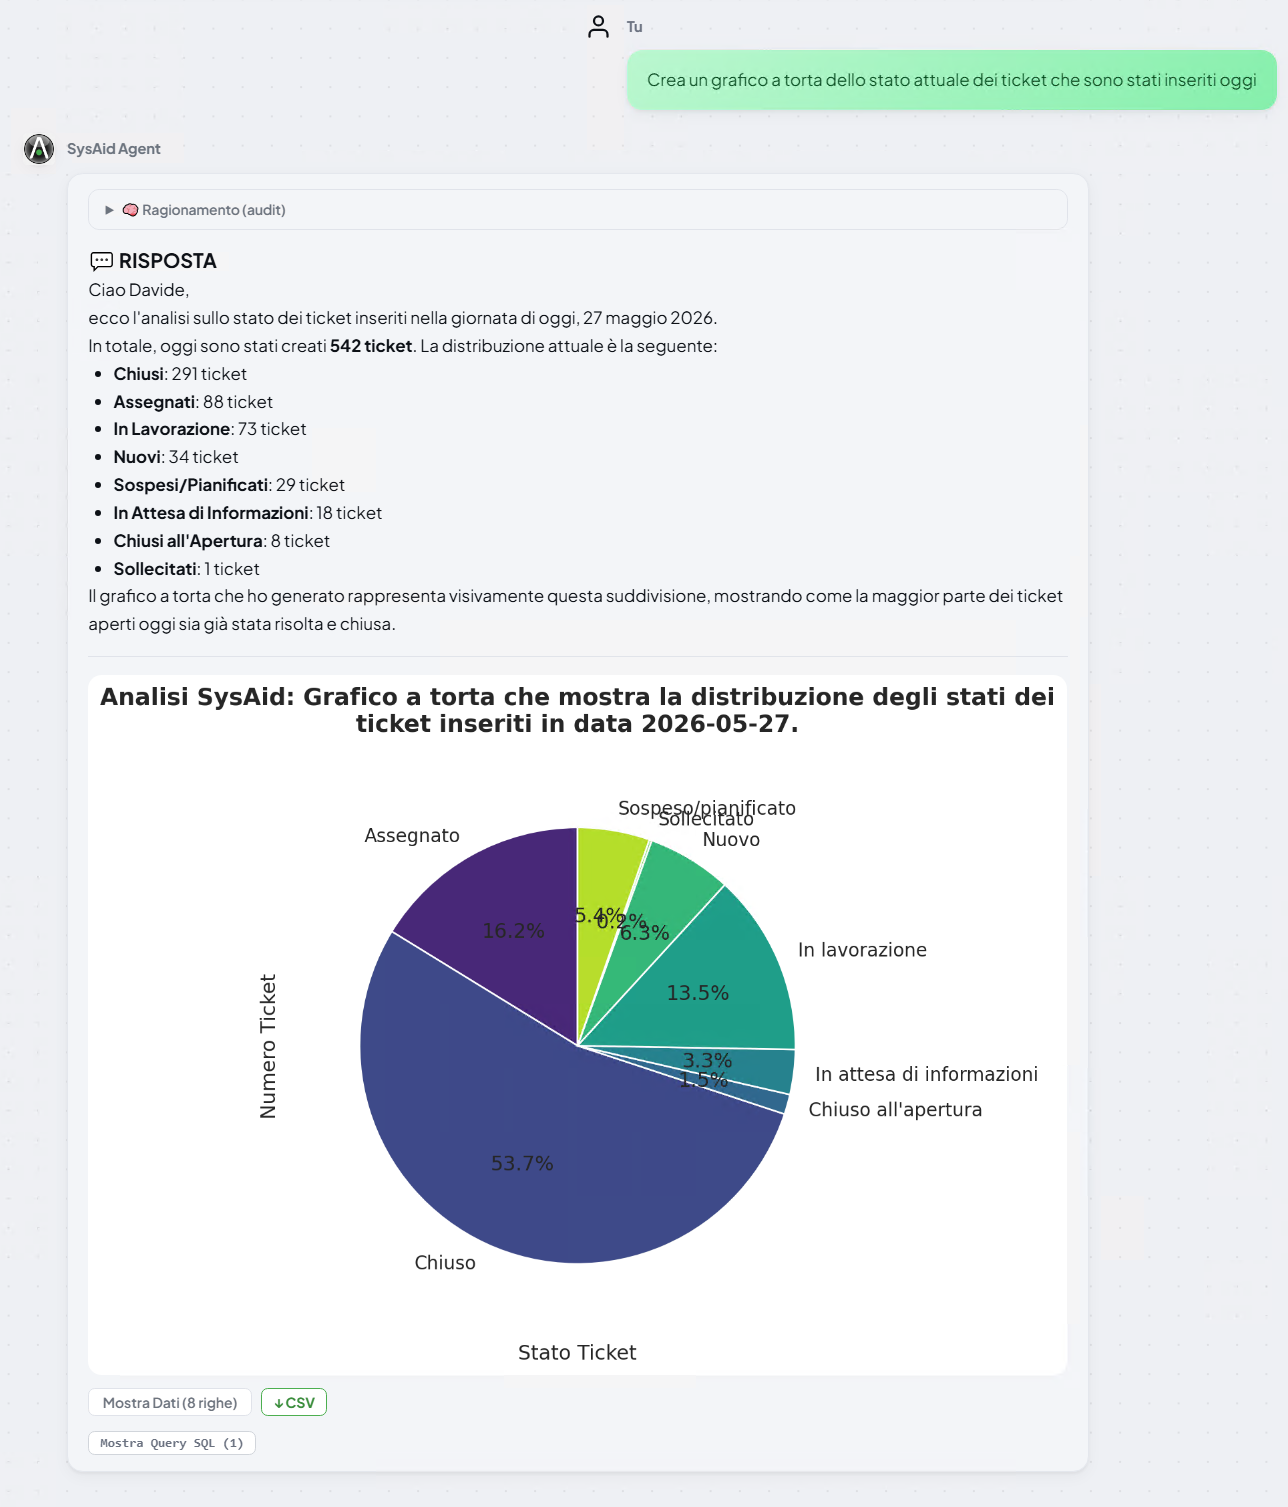
\includegraphics[width=0.68\textwidth,height=0.85\textheight,keepaspectratio]{sysaid3}
  \caption[Conversazione SysAid: code path Gemini Flash]{SysAid con code path Gemini~2.5 Flash per una richiesta a bassa complessità:
  la query SQL è eseguita con bassa latenza e il risultato è qui reso come grafico a torta della distribuzione degli stati dei ticket.}
  \label{fig:sysaid_conv_gemini}
\end{figure}

\begin{figure}[htbp]
  \centering
  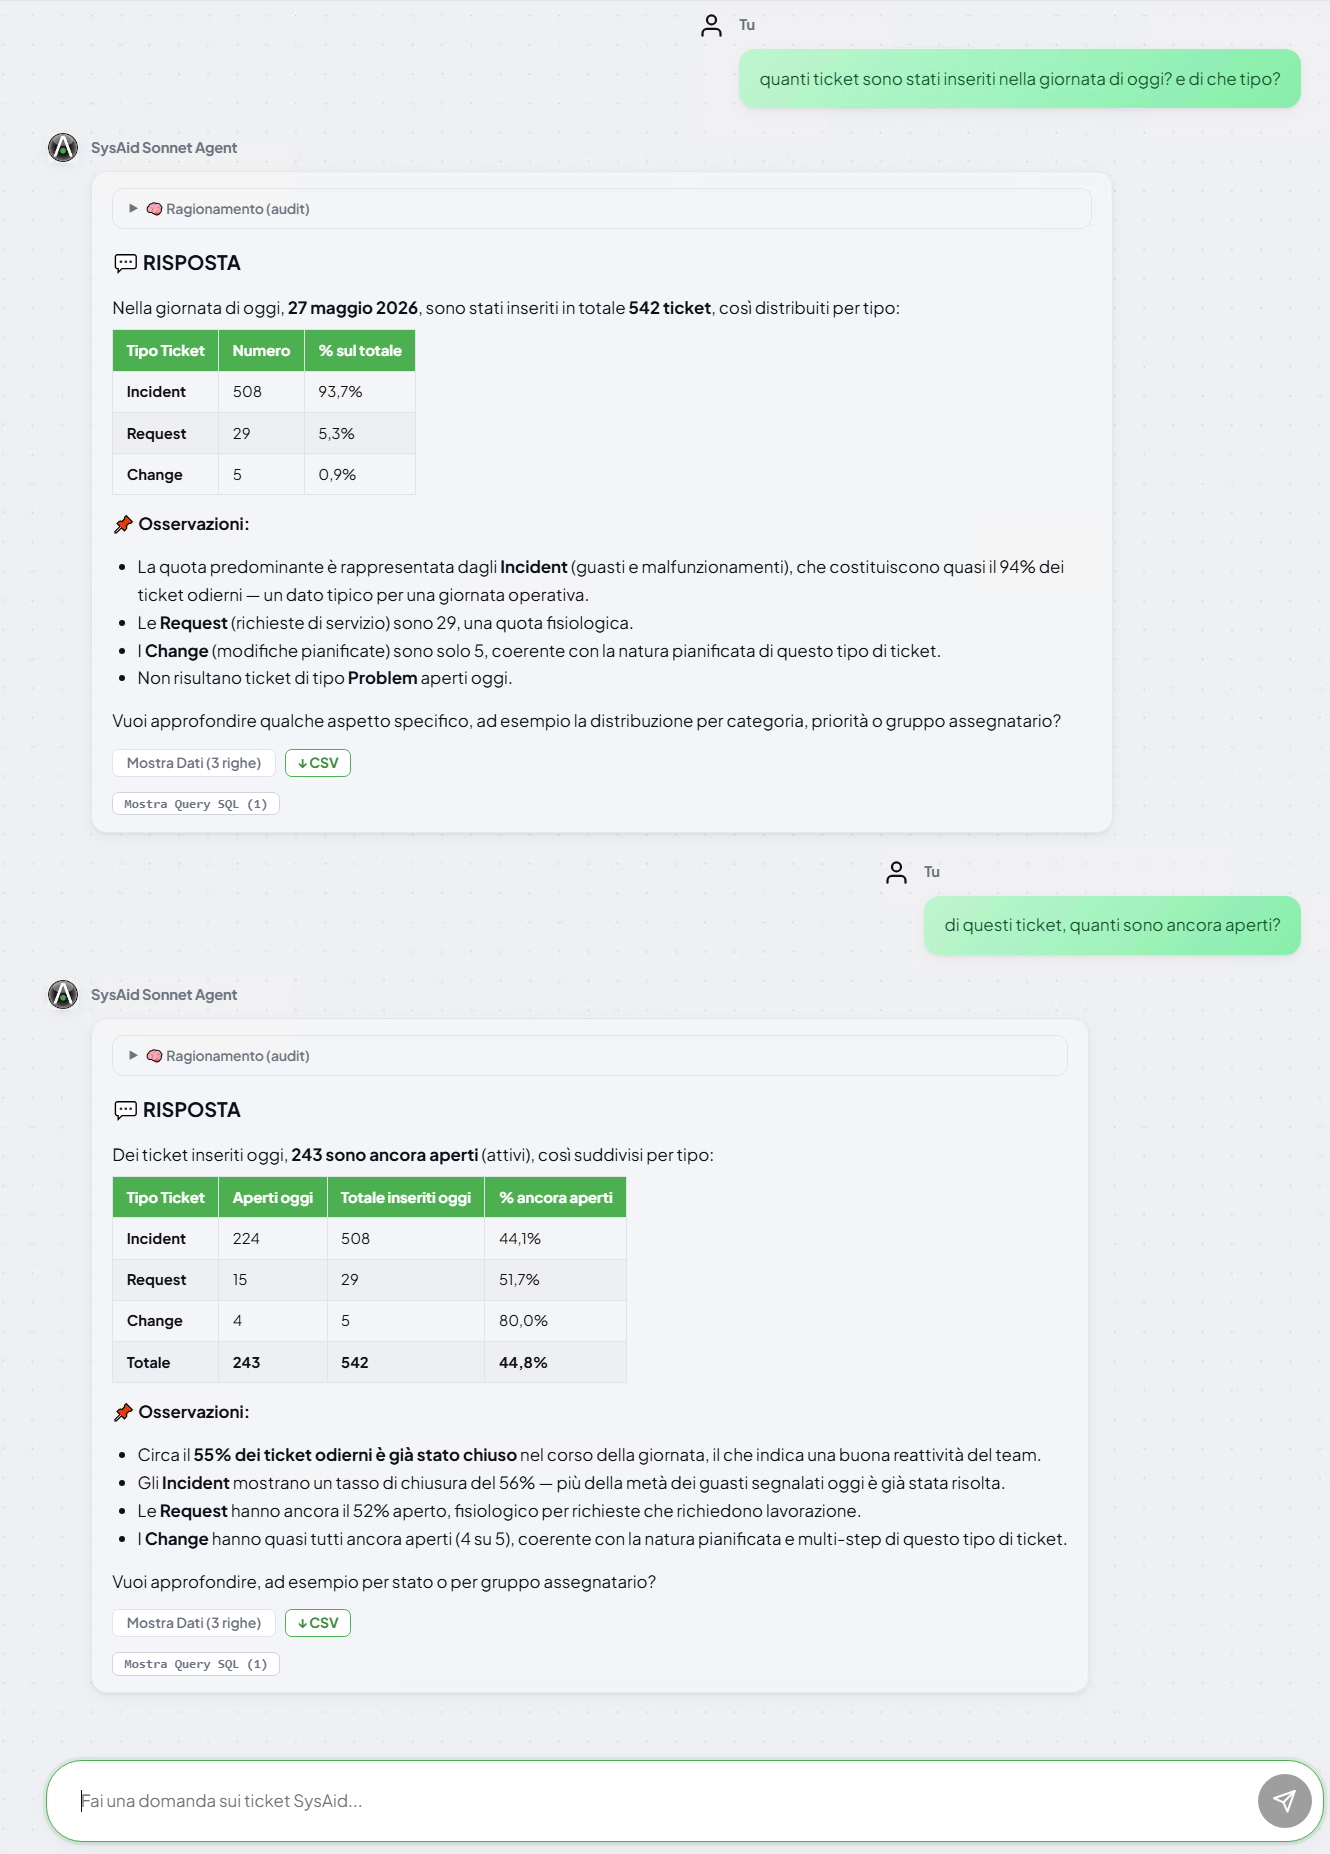
\includegraphics[width=0.68\textwidth,height=0.85\textheight,keepaspectratio]{sysaid2}
  \caption[Conversazione SysAid: code path Claude Sonnet]{SysAid con code path Claude Sonnet~4.6 per una richiesta ad alta complessità:
  la logica di business è identica alla code path Gemini; cambia solo il modello che esegue il ragionamento e la generazione SQL.}
  \label{fig:sysaid_conv_sonnet}
\end{figure}

% =====================================================================
\section{Pannello di amministrazione}
\label{sec:agenti-admin-impl}
% =====================================================================

Il monitoraggio e la configurazione della suite sono affidati a un pannello
di amministrazione dedicato a Vera (\texttt{admin-backend} +
\texttt{admin-frontend}),  isolato dagli applicativi
rivolti all'utente finale. Il backend FastAPI espone i propri router sotto
il prefisso \texttt{/api/admin/} e offre le seguenti funzionalità:
la gestione dei budget token per utente (con la tabella condivisa
\texttt{token\_budget} descritta sopra), le statistiche di consumo aggregate,
i log audit delle conversazioni con il feedback strutturato degli utenti,
la configurazione dei gruppi di esenzione PII e la gestione dei template
Model Armor e DLP (Sensitive Data Protection).

Il pannello di Orion, descritto nel
Cap.~\ref{chap:orion}, replica le stesse funzionalità
e aggiunge le pagine specifiche per la valutazione del routing.

La qualità di questi agenti (accuratezza delle query Text-to-SQL di
AllyCare e SysAid e fedeltà delle risposte RAG di CooPolicy) è valutata
nel Capitolo~\ref{chap:orion-valutazione}
(Sez.~\ref{sec:eval-agenti}).

% =====================================================================
\section{Alternative scartate}
\label{sec:agenti-alternative}
% =====================================================================

Questa sezione documenta le principali alternative considerate e le
ragioni per cui non sono state adottate.

\paragraph{Orchestratore centrale fin dalla versione~1.}
La prima alternativa valutata era introdurre un orchestratore
intelligente già nella versione iniziale della suite, ispirato
ai pattern multi-agente proposti dalla letteratura recente~\cite{wu2023autogen,guo2024multiagent,wang2024moa}, eliminando la
necessità per l'utente di selezionare esplicitamente l'agente. Questa
opzione è stata inizialmente scartata per una ragione metodologica: costruire
contemporaneamente gli agenti specializzati e il loro orchestratore
avrebbe reso molto più difficile isolare e diagnosticare i problemi e probabilmente avrebbe
condotto a performance degli agenti ``verticali'' molto meno ottimizzate.
Validare ogni agente indipendentemente è molto più semplice in un contesto ``verticale'' isolato.
L'orchestratore è stato quindi introdotto solo a valle della validazione
dei singoli agenti, ed è oggetto del Capitolo~\ref{chap:orion}.

\paragraph{Fine-tuning o training di un modello proprietario o open source.}
Si è valutato di addestrare un modello sui dati interni per creare un LLM specializzato sul dominio.
L'opzione è stata scartata per due ragioni. Primo, il costo di addestramento e mantenimento su scala
enterprise è proibitivo per un'organizzazione il cui core business non è lo sviluppo di modelli AI
(manca l'hardware adeguato e acquisirlo non sarebbe giustificabile). Secondo, il fine-tuning non
risolve il \emph{knowledge cutoff}: un modello addestrato sui dati di sei mesi fa non conosce i ticket
di questa settimana né le policy aggiornate ieri --- per i dati che cambiano nel tempo la risposta
corretta è il grounding.

% !TEX root = ../main.tex
% =====================================================================
% CAPITOLO 4 — ORION: L'ORCHESTRATORE
% (fusione dei precedenti capitoli "architettura" e "implementazione",
%  revisione giugno 2026 su indicazione dei relatori — vedi
%  plans/PIANO_REVISIONE_FEEDBACK.md, attività F1)
% =====================================================================

\chapter{Orion: l'orchestratore}
\label{chap:orion}

Questo capitolo presenta Orion, l'orchestratore che costituisce il
contributo conclusivo della tesi. Mentre il Capitolo~\ref{chap:agenti} ha
descritto la suite di agenti verticali come un insieme di servizi
indipendenti, ciascuno raggiungibile dall'utente attraverso il portale, qui
si affronta il problema complementare: come consentire all'utente di
interagire con \emph{un unico punto di accesso} che instradi automaticamente
ogni richiesta verso l'agente più competente. Ogni componente
dell'orchestratore --- routing step, agent proxy, gestione della
conversazione, frontend, pannello di amministrazione e infrastruttura --- è
presentato una sola volta, dalle scelte di progetto fino alla realizzazione.

% =====================================================================
\section{Motivazione e visione architetturale}
\label{sec:orion-motivazione}
% =====================================================================

L'approccio ad unico agente orchestratore consente il miglioramento della gestione di queste eventualità:

\paragraph{Errori di selezione.}
La selezione manuale introduce la possibilità di errore: l'utente sceglie l'agente sbagliato,
ottiene una risposta fuori dominio o un rifiuto, e deve ricominciare.


\paragraph{Richieste ibride.} Nella conversazione naturale, l'utente può passare fluidamente da un argomento
a un altro: ``Quanti ticket sono aperti oggi? E qual è l'NPS del negozio di Bologna?''.
Con agenti isolati, questa transizione richiede il cambio manuale di agente.

La visione di Orion è quella di un \emph{orchestratore intelligente} che elimina questi due limiti.
L'utente interagisce con un'unica interfaccia che analizza la richiesta, ne determina l'intento e la complessità,
e la inoltra in modo trasparente all'agente specializzato più appropriato.
Quando Orion non è sufficientemente sicuro della classificazione, pone una domanda di chiarimento prima di procedere,
in un meccanismo di disambiguazione \emph{human-in-the-loop} ispirato ai principi dell'\emph{active learning}~\cite{settles2012active,diao2023activeprompting}.

Il pattern architetturale di Orion è quello dell'\emph{orchestratore gerarchico} descritto nella letteratura sui sistemi multi-agente basati su
LLM~\cite{guo2024multiagent}: un \emph{supervisor agent} coordina $K$ agenti specializzati,
ciascuno con il proprio dominio di competenza, senza che gli agenti interagiscano direttamente tra loro.
Rispetto ai pattern cooperativi puri~\cite{wu2023autogen,wang2024moa}, l'architettura gerarchica ha il vantaggio
della semplicità operativa: il flusso è sempre \emph{utente} $\rightarrow$ \emph{router} $\rightarrow$ \emph{un solo agente} $\rightarrow$ \emph{risposta},
senza negoziazioni tra agenti che complicano il debugging e aumentano la latenza.

% =====================================================================
\section{Panoramica architetturale}
\label{sec:orion-panoramica}
% =====================================================================
\label{sec:orion-impl-multirepo}

La Fig.~\ref{fig:orion_architettura} riassume la vista d'insieme.
Una richiesta dell'utente segue un percorso lineare: il \emph{frontend} di Orion
la inoltra al \emph{backend}, che invoca il \emph{routing step} LLM-based (Sez.~\ref{sec:orion-routing});
questo seleziona in un solo passo l'agente competente all'interno dell'insieme disponibile (\texttt{self}, \texttt{sysaid}, \texttt{allycare}, \texttt{coopolicy}).
La richiesta è quindi inoltrata al backend del sub-agente selezionato tramite l'\emph{agent proxy} (Sez.~\ref{sec:orion-proxy}),
che ne normalizza la risposta prima di restituirla al frontend.

Il valore \texttt{self} non corrisponde a un sub-agente esterno,
ma alla pipeline generalista interna di Orion (clonata da Vera, vista in precedenza: RAG sui documenti caricati dall'utente, ricerca web e conoscenza parametrica)
che funge anche da \emph{fallback} quando un sub-agente non è raggiungibile.
Le sezioni successive approfondiscono i due componenti chiave, il routing step e l'agent proxy,
preceduti dal posizionamento rispetto ai sistemi affini (Sez.~\ref{sec:orion-related}).

\begin{figure}[htbp]
    \centering
    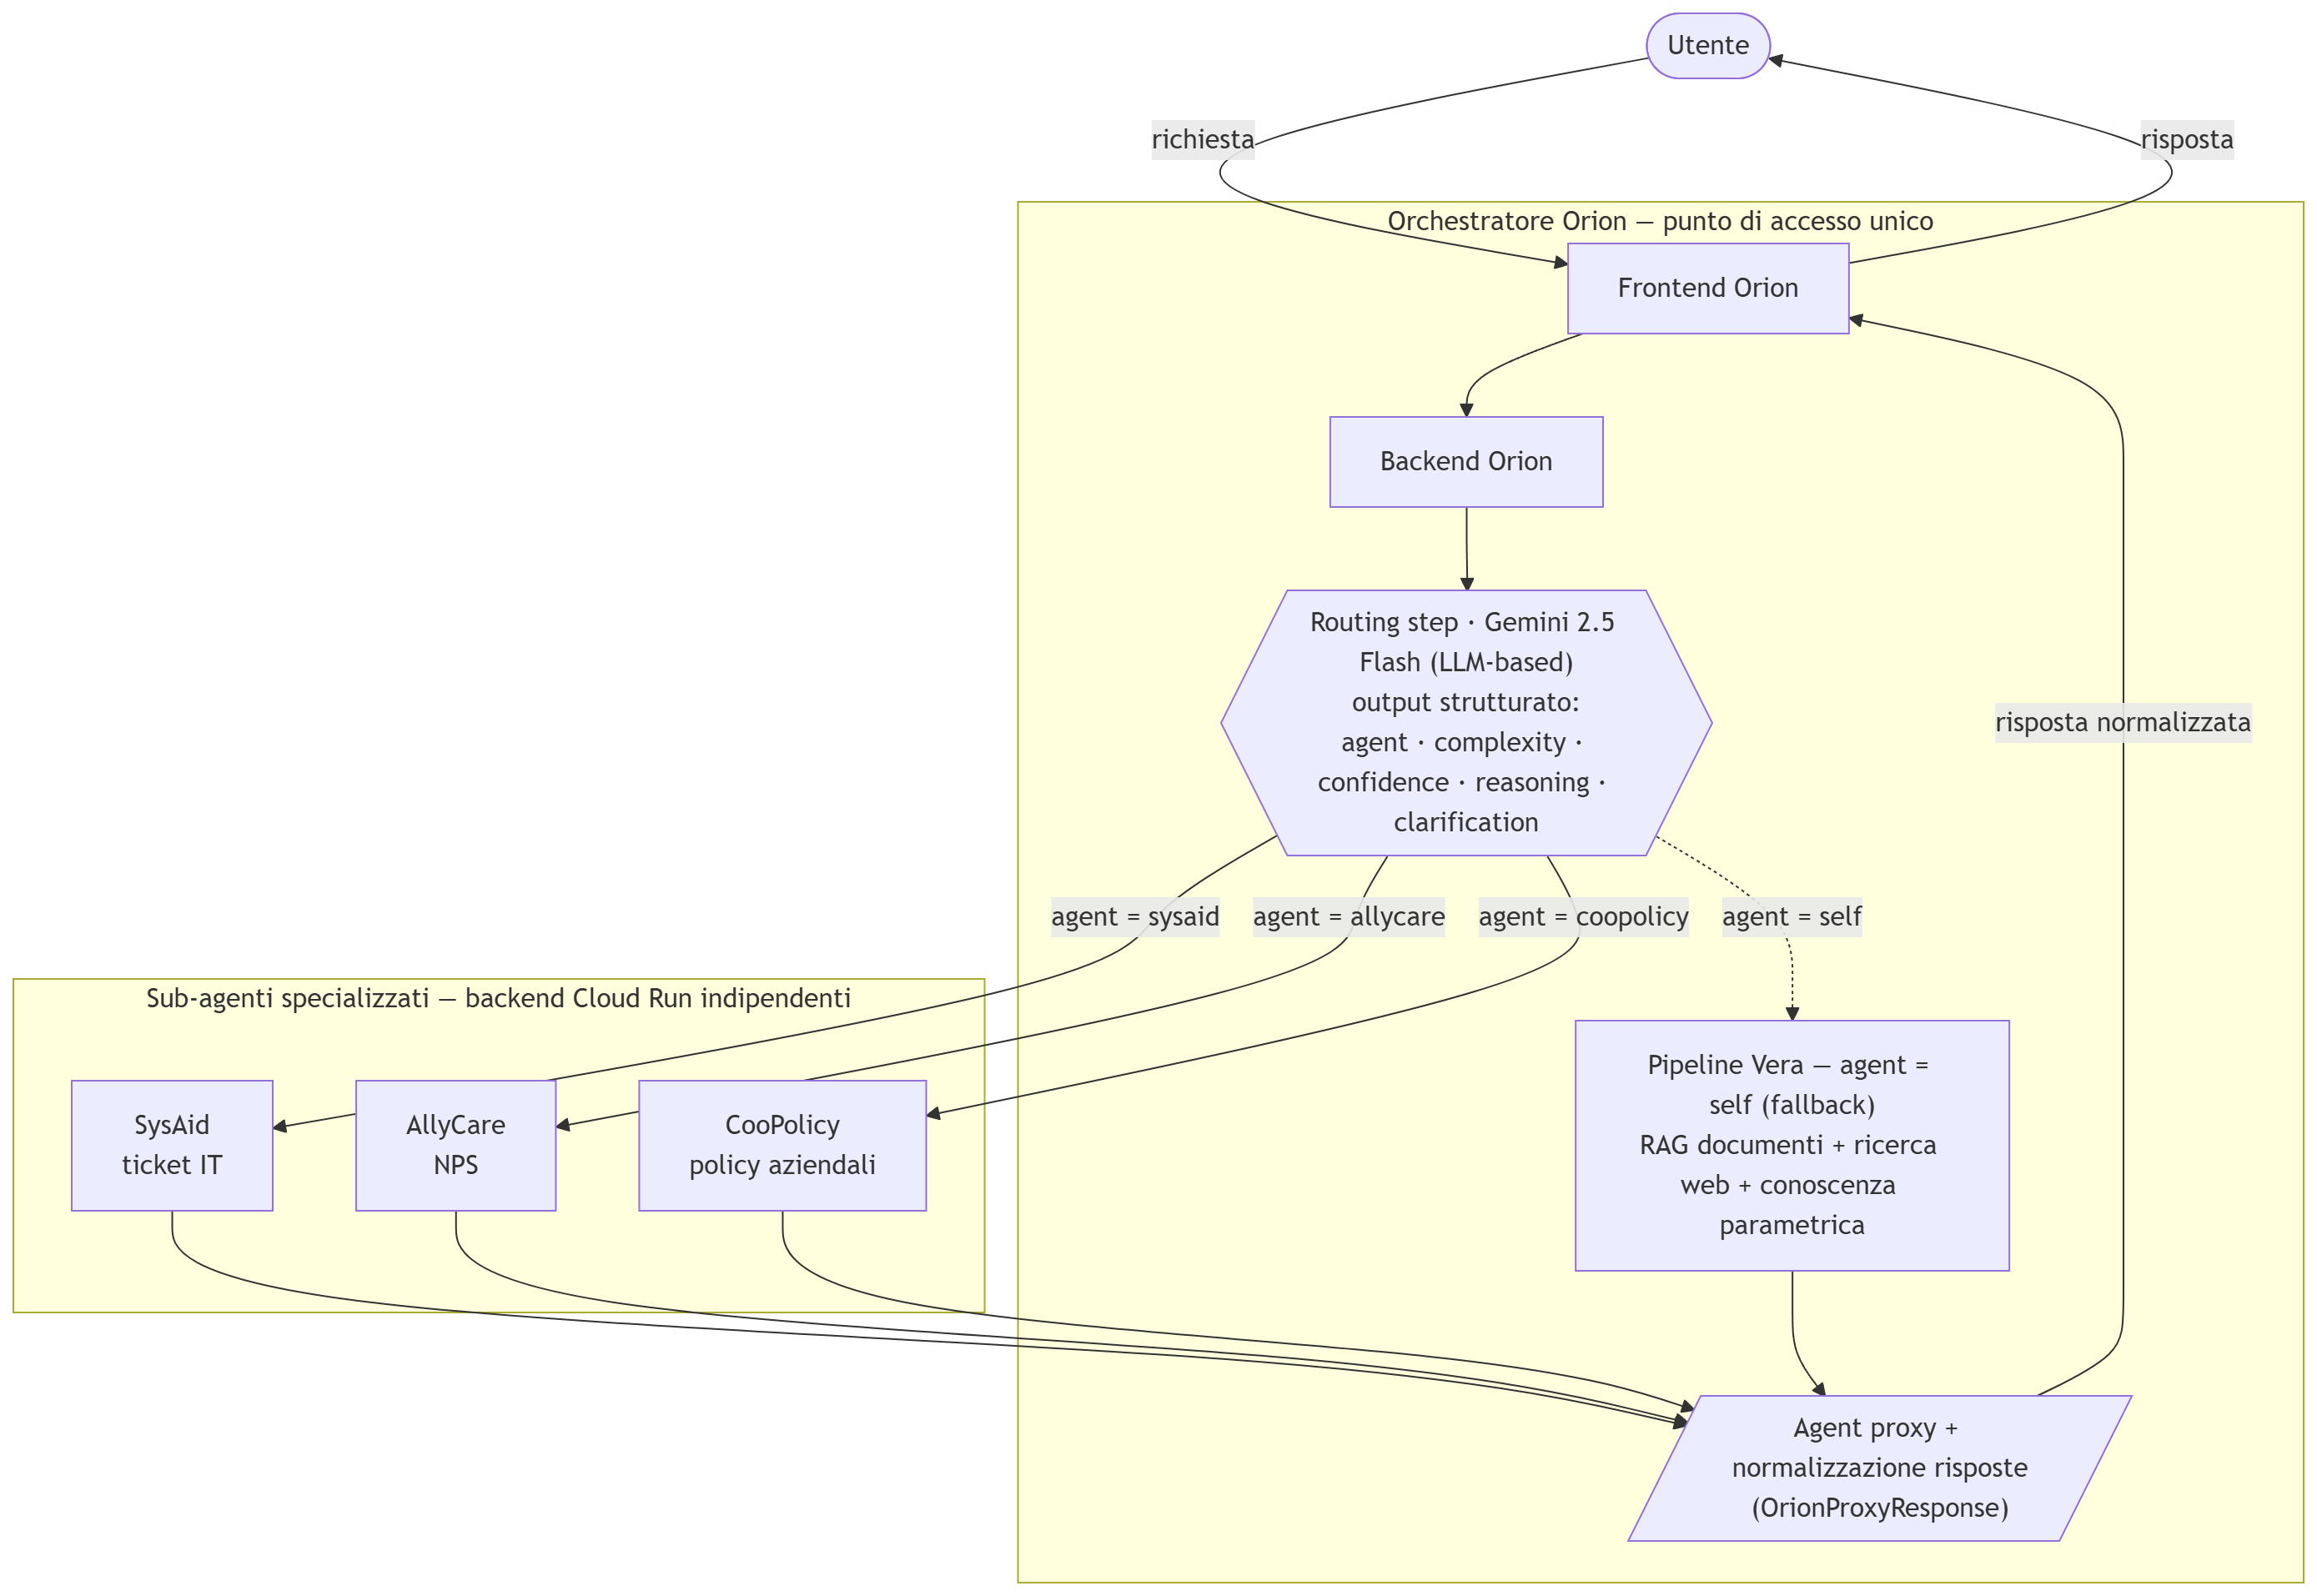
\includegraphics[width=\textwidth]{orion1}
    \caption[Architettura di Orion]{Architettura dell'orchestratore Orion: il routing step LLM-based seleziona dinamicamente quale agente specializzato invocare;
    il proxy normalizza le risposte; la pipeline Vera (RAG + web search) resta come fallback su \texttt{agent == "self"}.}
    \label{fig:orion_architettura}
\end{figure}

\begin{figure}[htbp]
    \centering
    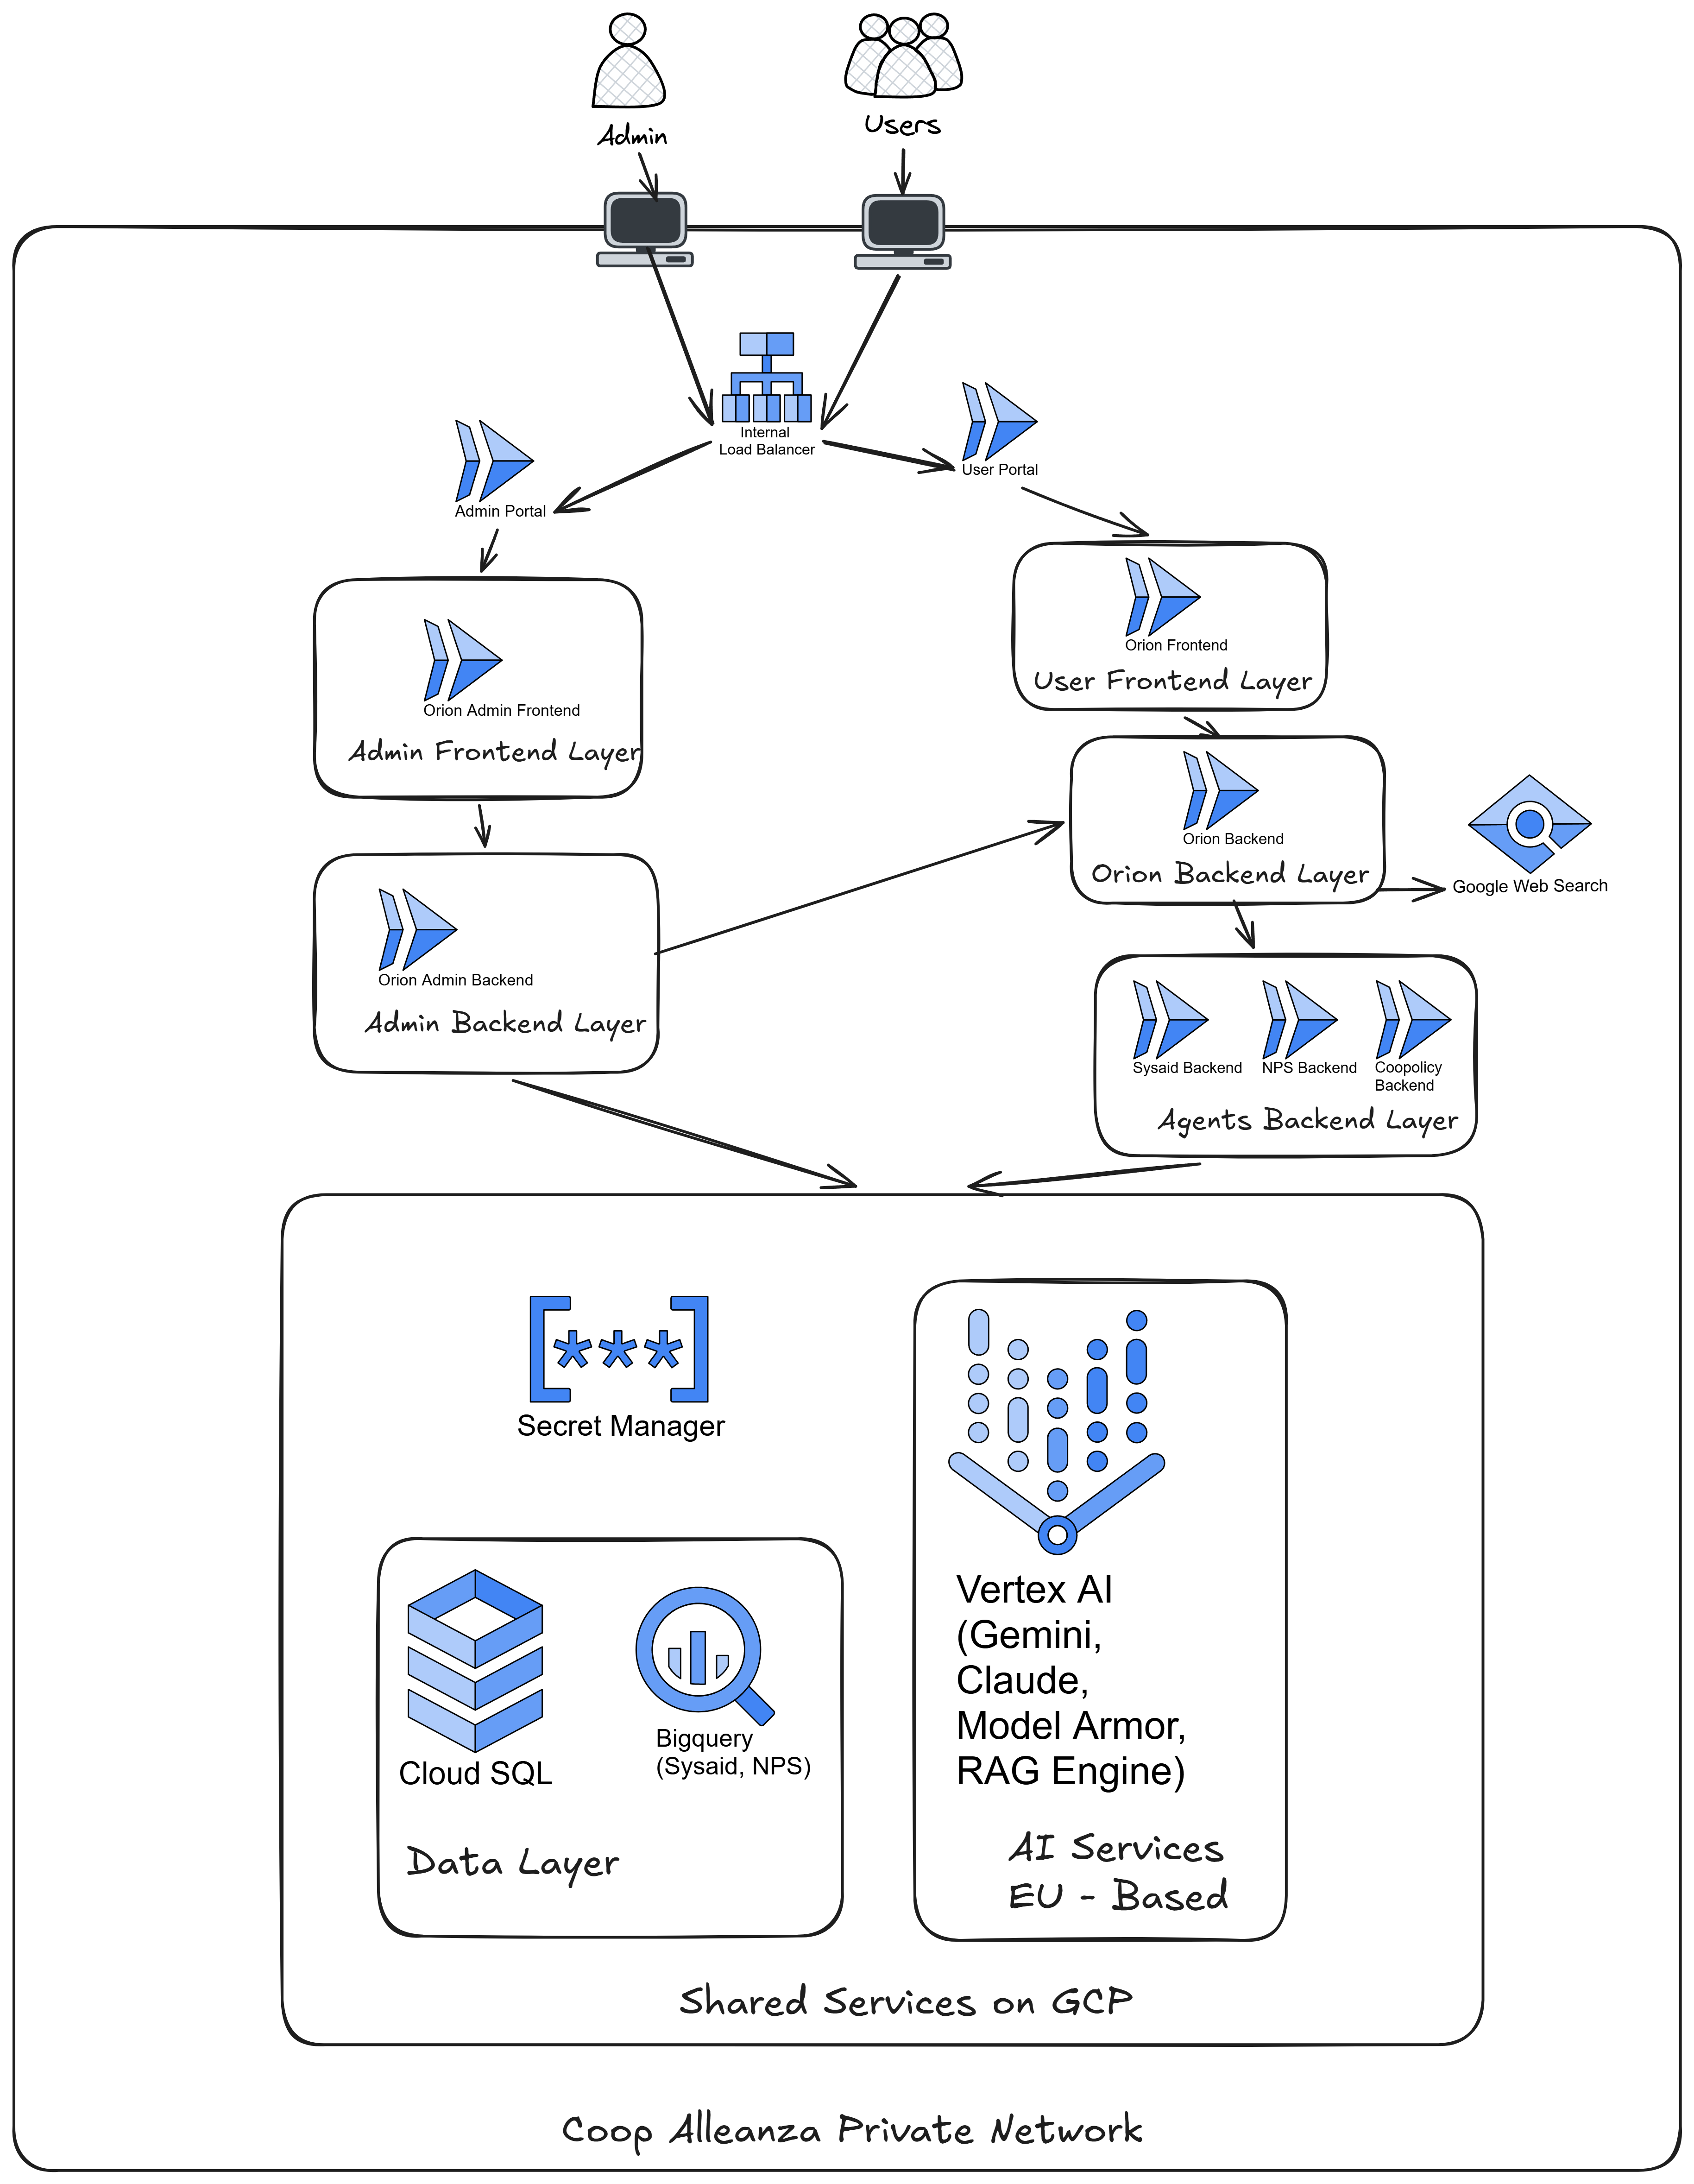
\includegraphics[width=0.9\textwidth,height=0.9\textheight,keepaspectratio]{diagrammaconorion}
    \caption[Architettura di sistema con Orion]{La suite nella sua forma finale, all'interno della rete privata di Coop Alleanza:
    un load balancer interno separa il percorso utente (Orion Frontend $\to$ Orion Backend $\to$ sub-agenti specializzati) dal percorso amministrativo,
    e tutti i backend condividono l'infrastruttura GCP (Cloud SQL, BigQuery, Secret Manager, Vertex AI con Gemini, Claude, Model Armor e RAG Engine).
    Evoluzione della Fig.~\ref{fig:architettura_suite} con l'aggiunta dello strato di orchestrazione.}
    \label{fig:architettura_orion_v2}
\end{figure}

Sul piano organizzativo, l'introduzione dell'orchestratore completa il
disegno obiettivo del progetto: ai repository della suite
(Fig.~\ref{fig:multirepo_tree}) si aggiungono quattro nuovi servizi dedicati
--- \texttt{orion-backend}, \texttt{orion-frontend},
\texttt{orion-admin-backend} e \texttt{orion-admin-frontend} --- ciascuno
con il proprio ciclo di CI/CD e i propri branch per ambiente, secondo lo
schema multi-repository già descritto (Sez.~\ref{subsec:agenti-multirepo}).

Il backend di Orion è stato sviluppato a partire dal backend di Vera;
rispetto a Vera, aggiunge tre componenti nuovi: il \emph{router agent},
il \emph{proxy} verso i sub-agenti e l'endpoint dedicato alla valutazione.
Tutti gli endpoint utente sono esposti sotto il prefisso \texttt{/api/orion/};
gli endpoint amministrativi sono serviti da un servizio Cloud Run dedicato (\texttt{orion-admin-backend}),
descritto nella Sez.~\ref{sec:orion-impl-admin}.

% =====================================================================
\section{Lavori correlati e posizionamento}
\label{sec:orion-related}
% =====================================================================

Prima di descrivere l'architettura nel dettaglio, è utile posizionare Orion rispetto ai principali sistemi di routing
e orchestrazione di LLM proposti nella letteratura recente.

La Tab.~\ref{tab:orion-related} riassume il confronto lungo cinque dimensioni.

\begin{table}[htbp]
  \centering
  \caption[Confronto con i lavori correlati]{Posizionamento di Orion rispetto ai principali sistemi di routing e orchestrazione multi-agente.}
  \label{tab:orion-related}
  \small
  \begin{tabular}{p{2.4cm}p{3cm}p{2.8cm}p{2.3cm}p{2.3cm}}
    \toprule
    \textbf{Sistema}   & \textbf{Tipo routing} & \textbf{Aggiunta\newline agenti} & \textbf{Confidence} & \textbf{Grounding} \\
    \midrule
    FrugalGPT~\cite{chen2023frugalgpt}
        & Cascade sequenziale    & Riordinamento coda  & Early-exit implicita  & Non previsto \\
    RouteLLM~\cite{ong2024routellm}
        & Classificatore appreso & Riaddestramento     & Non esplicita         & Non previsto \\
    AutoGen~\cite{wu2023autogen}
        & Cooperativo (chat)     & Registrazione agente & Non prevista         & A carico agente \\
    MoA~\cite{wang2024moa}
        & Competitivo + aggr.    & Aggiunta al pool    & Aggregazione          & Non previsto \\
    \textbf{Orion}
        & LLM-based strutturato  & Aggiornamento prompt & Esplicita + clarif.  & Eterogeneo \\
    \bottomrule
  \end{tabular}
\end{table}

\paragraph{Orion vs FrugalGPT.} FrugalGPT~\cite{chen2023frugalgpt}
formalizza il routing come un \emph{cascade}: i modelli sono ordinati per costo crescente
e la richiesta scala al modello successivo solo se il precedente non è abbastanza sicuro.
Orion non è un cascade ma un \emph{router diretto}: il routing step seleziona un singolo agente in un solo passo, senza prove sequenziali.
Il vantaggio è una latenza prevedibile e indipendente dal numero di agenti; lo svantaggio è che la decisione è irreversibile nel turno.

\paragraph{Orion vs RouteLLM.} RouteLLM~\cite{ong2024routellm} addestra un classificatore su dati
di preferenza umana per decidere tra un modello forte e uno debole.
Orion affronta un problema più ampio (selezione tra $K$~agenti eterogenei,
non tra due modelli) e adotta un router LLM-based anziché appreso. Il trade-off è esplicito:
flessibilità (aggiungere un agente richiede l'aggiornamento del prompt, non il riaddestramento)
contro efficienza (una chiamata LLM per ogni richiesta).
La transizione verso un router appreso è discussa come sviluppo futuro (Sez.~\ref{subsec:concl-routellm}).

\paragraph{Orion vs AutoGen.} AutoGen~\cite{wu2023autogen} implementa un pattern cooperativo in cui gli agenti
dialogano tra loro attraverso un \texttt{GroupChatManager}. Orion adotta un pattern strettamente gerarchico:
il flusso unidirezionale già descritto (Sez.~\ref{sec:orion-motivazione}) resta l'unica via,
senza interazione inter-agente. La semplicità del flusso lineare è un requisito in contesto enterprise,
dove la tracciabilità di ogni decisione e la prevedibilità della latenza sono prioritarie rispetto alla flessibilità compositiva.

\paragraph{Orion vs Mixture-of-Agents.} MoA~\cite{wang2024moa} sottopone la stessa richiesta a $N$~agenti e aggrega le risposte.
Orion seleziona un singolo agente, evitando il costo computazionale di $N$~invocazioni parallele.
L'approccio è giustificato dal fatto che gli agenti della suite operano su fonti dati disgiunte:
aggregare una risposta RAG con una risposta Text-to-SQL non produrrebbe una risposta migliore, ma solo rumore.

\paragraph{Specificità di Orion.} Due caratteristiche distinguono Orion dai sistemi citati: (i)~l'output
strutturato del router include un \emph{confidence score} esplicito con soglia configurabile e meccanismo di \emph{clarification},
implementando una forma di \emph{deferral} basato sull'incertezza, ispirato ai principi dell'\emph{active learning}
ma operante in fase di inferenza (\emph{human-in-the-loop}) anziché come ciclo di ri-addestramento; (ii)~gli agenti orchestrati utilizzano forme di
grounding eterogenee (Web, RAG, Text-to-SQL), una dimensione assente nei lavori citati,
che si concentrano sulla selezione del modello piuttosto che sulla selezione della \emph{fonte di conoscenza}.

% =====================================================================
\section{Il routing step: stima di intento, complessità, confidenza}
\label{sec:orion-routing}
% =====================================================================

Il cuore di Orion è il \emph{routing step}: un modulo che,
dato il prompt dell'utente e l'eventuale cronologia della conversazione,
produce una decisione di instradamento sotto forma di oggetto strutturato.
La scelta di delegare il routing a un LLM, anziché a un classificatore addestrato ad hoc,
è motivata da tre ragioni pratiche: (i)~il set di agenti target evolve nel tempo
 e non si desidera riaddestrare un modello a ogni aggiunta; (ii)~il reasoning esplicito del modello
 fornisce tracciabilità diagnostica per ogni decisione; (iii)~il costo di una singola chiamata
 a un modello veloce ed economico (Gemini~2.5 Flash) è trascurabile rispetto al costo
 della risposta completa dell'agente invocato.

\subsection{Output strutturato del router}
\label{subsec:orion-output-strutturato}

Il router produce un oggetto JSON vincolato,
utilizzando il meccanismo di \emph{guided generation}~\cite{willard2023outlines} offerto dall'API di
Vertex AI (\texttt{response\_mime\_type = "application/json"} con \texttt{response\_schema} esplicito).
Lo schema, definito dal modello Pydantic che valida l'output della funzione
\texttt{classify} (Sez.~\ref{subsec:orion-impl-router}), è il seguente:

\begin{lstlisting}[language=Python,caption={Schema dell'output strutturato del router e firma della funzione \texttt{classify}.},label={lst:classify-signature}]
class RouterOutput(BaseModel):
    agent: str        # "self" | "sysaid" | "allycare" | "coopolicy"
    complexity: str   # "low" | "high"
    confidence: float # 0.0 .. 1.0
    reasoning: str    # Chain-of-Thought esplicita
    clarification_needed: Optional[str] = None

async def classify(
    prompt: str,
    history: list,
    available_agents: list[str],
) -> RouterOutput:
\end{lstlisting}

Ogni campo assolve a una funzione precisa:

\begin{description}
  \item[\texttt{agent}] Identificatore dell'agente target.
  Il campo è vincolato a un'\texttt{enum} contenente i soli agenti disponibili per l'utente corrente,
  garantendo che il modello non possa inventare target inesistenti.
  Il valore \texttt{"self"} indica che Orion gestisce la richiesta internamente
  (RAG su documenti caricati dall'utente, ricerca web, conoscenza parametrica).

  \item[\texttt{complexity}] Stima binaria della complessità della richiesta: \texttt{"low"} per domande dirette,
  conteggi semplici, filtri base; \texttt{"high"} per analisi multi-dimensionali, correlazioni,
  confronti temporali articolati, report executive.
  La complessità non influenza la scelta dell'agente ma è propagata al sub-agente nel
  payload della richiesta, che la utilizza per il proprio \emph{model routing} interno (cfr. Sez.~\ref{subsec:agenti-sysaid-confronto}),
  realizzando il trade-off costo--qualità descritto nella Sez.~\ref{sec:bg-routing}.

  \item[\texttt{confidence}] Valore numerico nell'intervallo $[0, 1]$
  che esprime la certezza del router nella classificazione effettuata.
  Il campo è il fondamento del meccanismo di \emph{clarification} descritto nella sezione successiva.

  \item[\texttt{reasoning}] Catena di ragionamento esplicita (\emph{Chain-of-Thought}~\cite{wei2022cot})
  che il modello è istruito a produrre prima della decisione.
  Il campo non viene mostrato all'utente ma è persistito nel log di routing e
  consultabile dall'amministratore attraverso il pannello di amministrazione,
  abilitando un ciclo di miglioramento continuo del prompt.

  \item[\texttt{clarification\_needed}] Domanda di chiarimento da porre all'utente quando la confidence è insufficiente.
  Quando valorizzato, il routing non procede: Orion restituisce la domanda all'utente e
  attende un nuovo turno conversazionale prima di classificare nuovamente.

\end{description}

\subsection{Logica di confidence e clarification}
\label{subsec:orion-confidence}

La \emph{confidence} prodotta dal router governa il comportamento del
sistema secondo una logica a soglia configurabile.
La soglia di default, \texttt{ROUTER\_CONFIDENCE\_THRESHOLD}, è impostata a 0,60 (modificabile):

\begin{itemize}
  \item Se $\text{confidence} \geq \text{threshold}$, il routing procede normalmente: la richiesta è inoltrata all'agente selezionato.
  \item Se $\text{confidence} < \text{threshold}$, il routing è sospeso. Se il modello ha già proposto una domanda di chiarimento (\texttt{clarification\_needed} non nullo), essa viene restituita all'utente. In caso contrario, il sistema genera automaticamente una richiesta di disambiguazione generica.
\end{itemize}

La calibrazione del confidence score, la proprietà per cui il modello è
più incerto quando sbaglia e più sicuro quando ha ragione, non è banale;
la letteratura mostra che i modelli di grande scala sono ``ragionevolmente'' calibrati quando interrogati
esplicitamente sulla propria certezza~\cite{kadavath2022knowsknows}, ma la calibrazione peggiora su domini
specifici non visti in addestramento. Il Capitolo~\ref{chap:orion-valutazione} verifica empiricamente questa proprietà sul dominio del progetto.

\begin{figure}[htbp]
    \centering
    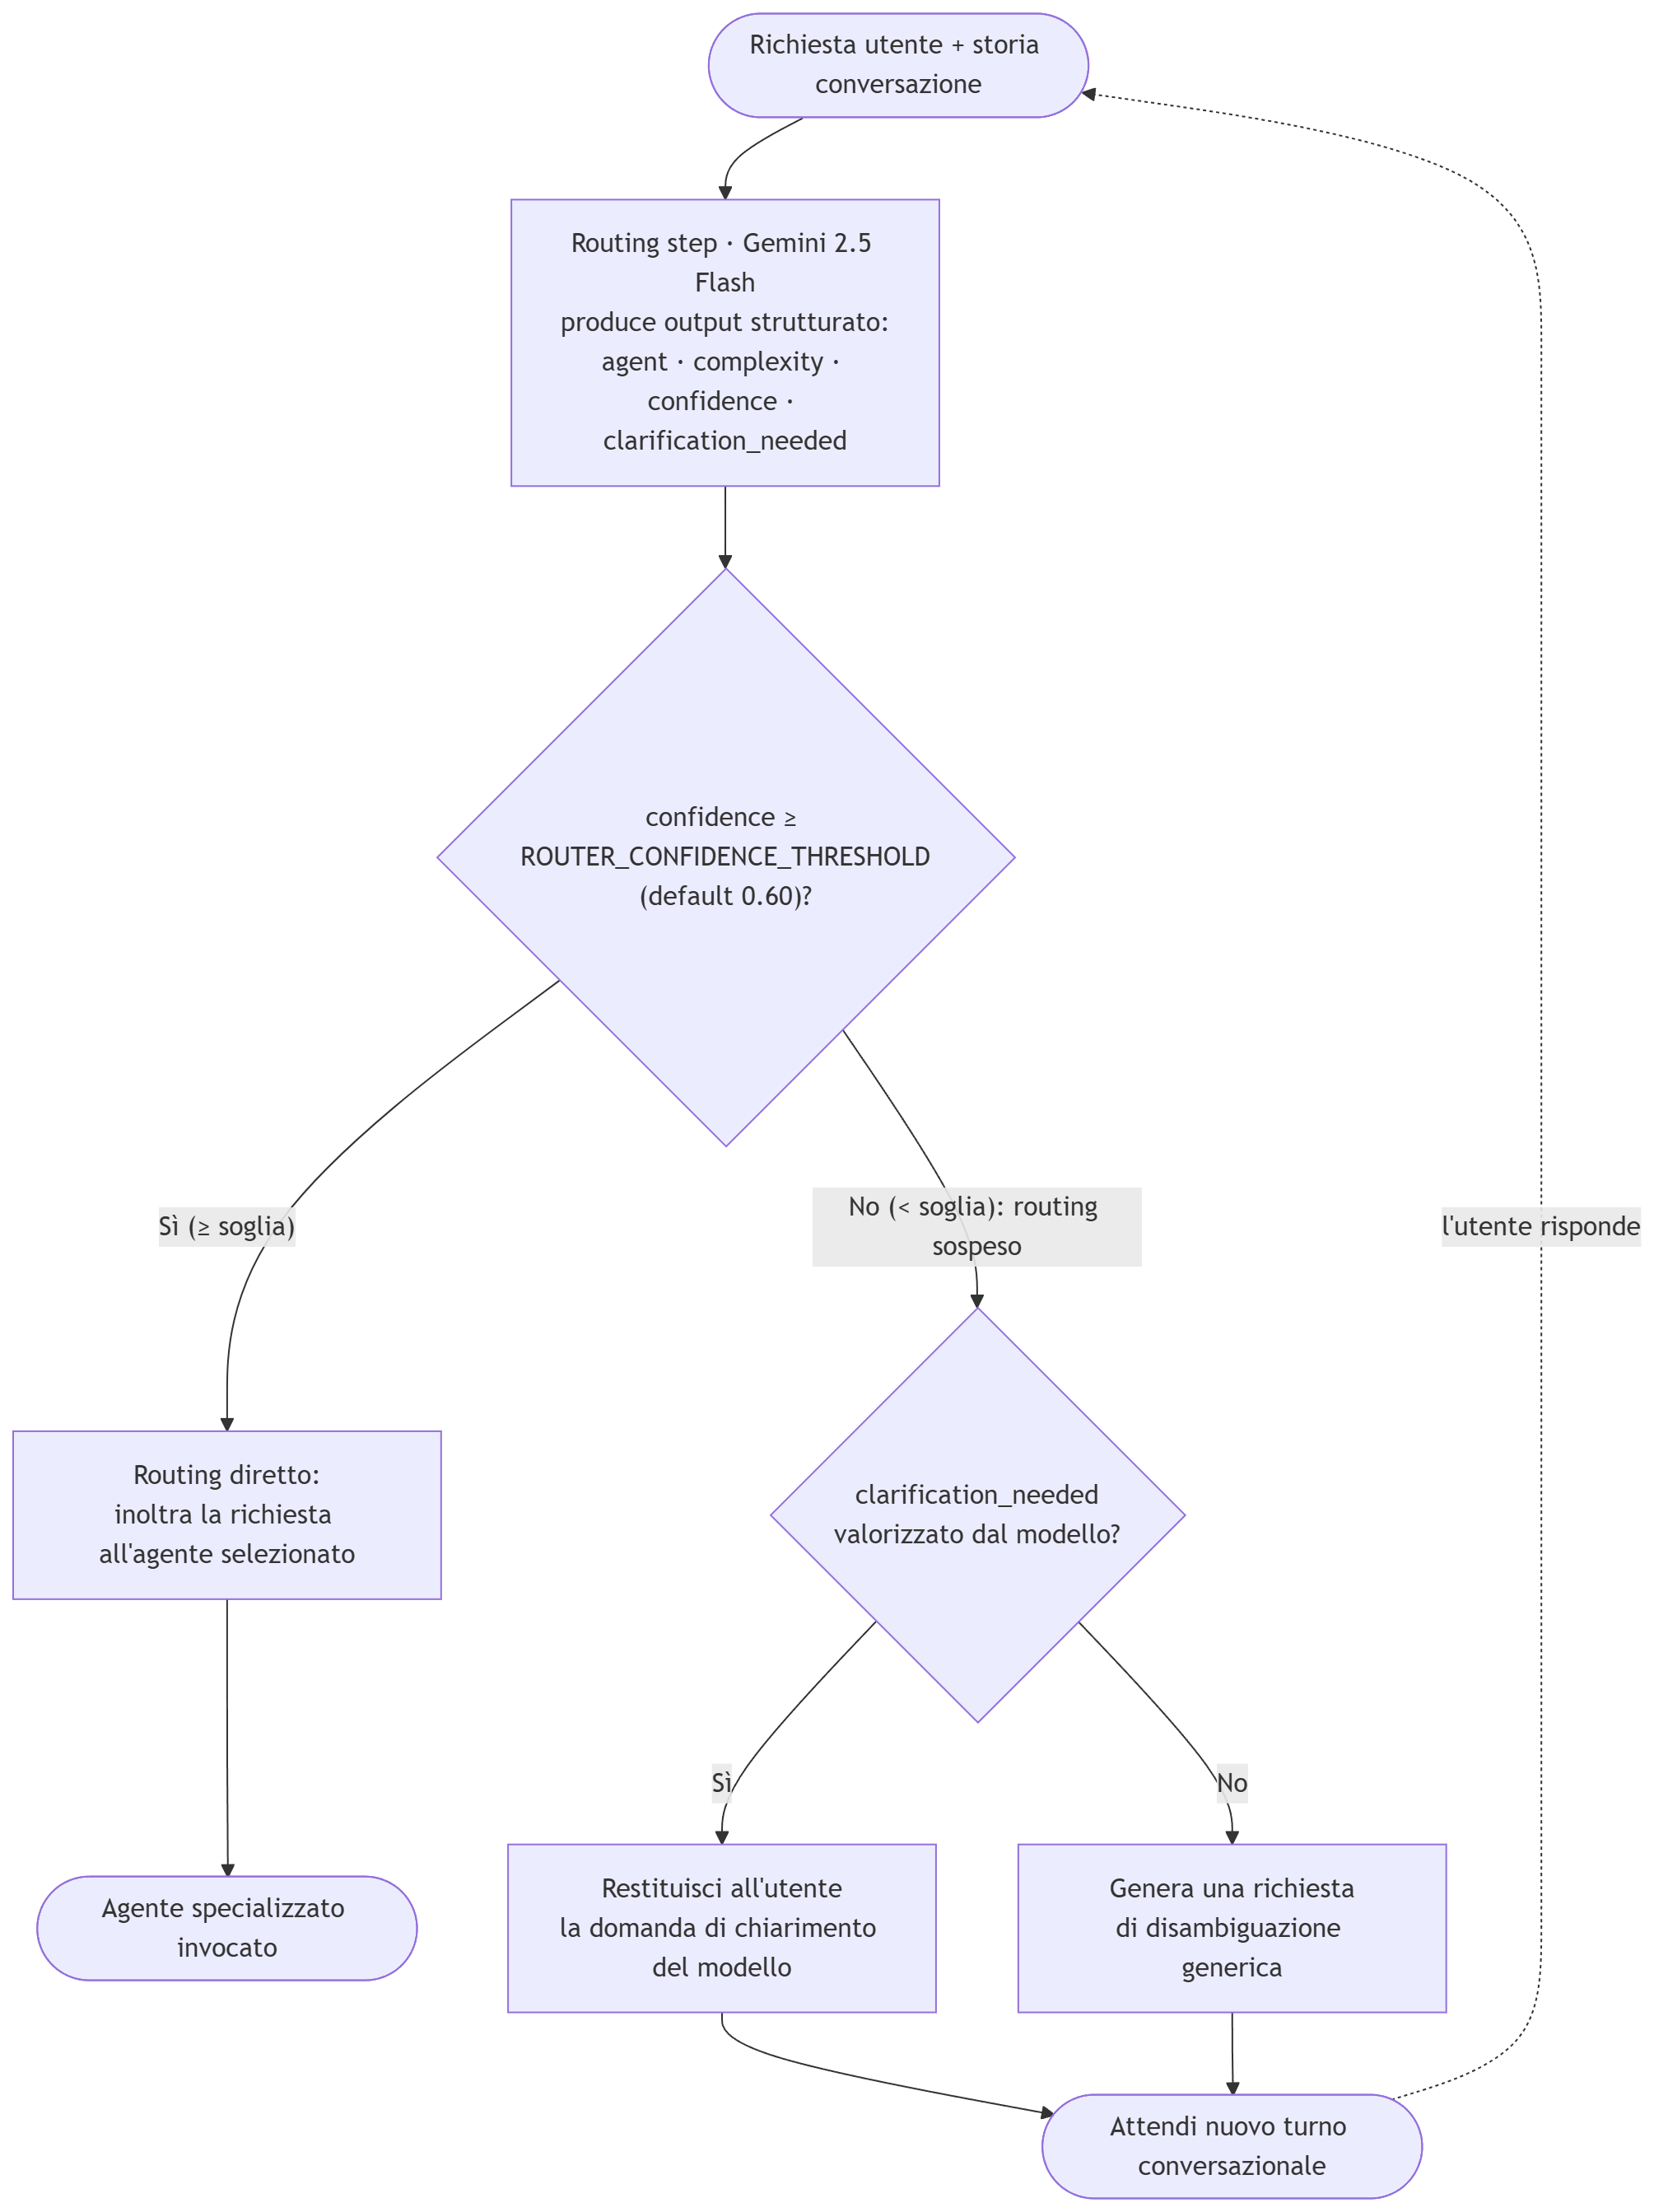
\includegraphics[height=0.85\textheight,keepaspectratio]{orion2}
    \caption[Routing decision flow]{Logica di routing: in funzione della soglia di confidenza configurabile, Orion instrada direttamente oppure pone all'utente una domanda di chiarimento.}
    \label{fig:routing_decision}
\end{figure}

\subsection{Scelta del modello per il routing}
\label{subsec:orion-model-routing}

Il modello utilizzato per il routing step è Gemini~2.5 Flash~\cite{team2024gemini}.
La scelta è motivata da tre fattori:

\begin{enumerate}
  \item \textbf{Latenza.} Il routing step aggiunge latenza all'intera pipeline:
  il tempo trascorso tra la richiesta dell'utente e l'inizio della risposta è la somma della latenza del router e della latenza dell'agente.
  Con Gemini Flash, il modello più rapido della famiglia, la latenza aggiunta dal routing step è contenuta e trascurabile rispetto al tempo di generazione della risposta completa dell'agente.
  \item \textbf{Costo.} Il router è chiamato su \emph{ogni} richiesta utente. Un modello più potente (ad esempio Gemini~2.5 Pro o Claude Sonnet) avrebbe un costo unitario superiore,
  che moltiplicato per il volume di traffico rischia di diventare impattante.
  \item \textbf{Capacità sufficiente.} Il task del router è una classificazione
  vincolata su un set chiuso di $K$~etichette (quattro agenti + la variabile di complessità), con ragionamento esplicito.
  Un modello ``flash'' dovrebbe sempre essere sufficiente per questo tipo di compito,
  come confermato dai risultati sperimentali del Capitolo~\ref{chap:orion-valutazione}.
\end{enumerate}

L'alternativa di un router appreso, come RouteLLM~\cite{ong2024routellm} (Sez.~\ref{sec:bg-routing}),
è stata valutata come possibile evoluzione futura una volta che il sistema
sarà passato in produzione a tutti gli effetti, con l'aumento del volume di traffico
che potrebbe generare un dataset di training significativo.

\subsection{La funzione \texttt{classify}}
\label{subsec:orion-impl-router}

Il modulo \texttt{router\_agent.py} implementa il routing step nella funzione
asincrona \texttt{classify}, che riceve tre parametri: il prompt dell'utente,
la cronologia della conversazione (ultimi sei turni) e la lista degli agenti
disponibili. Il processo di classificazione si articola in quattro fasi:

\begin{enumerate}
  \item \textbf{Costruzione del prompt.} Il sistema compone il prompt completo
  concatenando il \emph{system prompt} del router (che descrive le regole di classificazione,
  la semantica della confidence e le istruzioni per il reasoning),
  il blocco descrittivo degli agenti disponibili (nome, descrizione, esempi di richieste tipiche per ciascuno)
  e il prompt dell'utente. La cronologia della conversazione è inclusa in forma sintetica
  (ultimi sei turni, ciascuno troncato a 200~caratteri, configurabile) per consentire al modello di risolvere
  riferimenti incrociati nei turni di \emph{follow-up}.

  \item \textbf{Chiamata a Vertex AI con output strutturato.} La funzione invoca Gemini~2.5 Flash
  attraverso il client \texttt{google.genai}, configurato con \texttt{temperature = 0.1} (più deterministico),
  \texttt{max\_output\_tokens = 1024} e il vincolo di \emph{guided generation} sullo schema
  già descritto (Sez.~\ref{subsec:orion-output-strutturato}), con l'\texttt{enum} del campo
  \texttt{agent} ristretta ai soli agenti passati come parametro.

  \item \textbf{Parsing e validazione.} La risposta JSON viene parsificata e
  validata attraverso il modello Pydantic \texttt{RouterOutput}.
  Se l'agente restituito non è nella lista degli agenti disponibili (possibile in caso di allucinazione residua nonostante lo schema),
  il sistema effettua un \emph{fallback} su \texttt{"self"}. Se la confidence è inferiore alla soglia configurata e il modello non ha proposto una domanda di chiarimento,
  il sistema ne genera una automaticamente.

  \item \textbf{Logging.} La decisione di routing viene loggata con livello \texttt{INFO}
  se la confidence è $\geq 0{,}80$, \texttt{WARNING} altrimenti. Il log include agente selezionato, complessità,
  confidence e flag di clarification, e alimenta la pagina \emph{Routing Logs} del pannello di amministrazione.
\end{enumerate}

In caso di eccezione durante la classificazione (errore di rete, timeout verso Vertex AI, errore di parsing),
il modulo restituisce un \emph{fallback deterministico}: \texttt{agent = "self"}, \texttt{confidence = 1.0},
con un reasoning che documenta l'errore.

\paragraph{Endpoint di valutazione.}
\label{subsec:orion-impl-classify}
L'endpoint \texttt{POST /api/orion/classify} espone il solo routing step, senza eseguire la risposta dell'agente selezionato.
Riceve un prompt e una storia opzionale, e restituisce l'output strutturato del router.
L'endpoint è stato progettato specificamente per il framework di valutazione descritto nel Capitolo~\ref{chap:orion-valutazione}:
testare il router in isolamento consente di eseguire centinaia di test case con il costo di una sola chiamata Flash per test case, senza attivare i sub-agenti.

% =====================================================================
\section{Agent proxy e normalizzazione delle risposte}
\label{sec:orion-proxy}
% =====================================================================
\label{subsec:orion-impl-proxy}

Una volta che il router ha selezionato l'agente target, il \emph{proxy} di Orion inoltra
la richiesta al backend del sub-agente via HTTP e normalizza la risposta prima di restituirla al frontend.
Il proxy è il componente che rende trasparente al frontend l'eterogeneità dei sub-agenti:
ogni agente ha il proprio formato di risposta (SysAid include query SQL e grafici base64; CooPolicy include citazioni con URI ai documenti; AllyCare include tabelle dati),
e il proxy li mappa verso una \emph{shape} uniforme.

Il modulo \texttt{agent\_proxy.py} implementa questa logica nella funzione
\texttt{forward}. La tabella degli endpoint è configurata tramite variabili
d'ambiente, una per ciascun sub-agente:

\begin{table}[htbp]
  \centering
  \caption[Mapping degli endpoint dei sub-agenti]{Mapping tra agente target, variabile d'ambiente per l'URL del backend e path dell'endpoint.}
  \label{tab:agent-endpoints}
  \begin{tabular}{lll}
    \toprule
    \textbf{Agent key} & \textbf{Env var}             & \textbf{Path} \\
    \midrule
    \texttt{sysaid}    & \texttt{SYSAID\_BACKEND\_URL} & \texttt{/api/sysaid/prompt} \\
    \texttt{allycare}  & \texttt{NPS\_BACKEND\_URL}    & \texttt{/api/nps/prompt} \\
    \texttt{coopolicy} & \texttt{DOCS\_BACKEND\_URL}   & \texttt{/api/docs/prompt} \\
    \bottomrule
  \end{tabular}
\end{table}

Il payload inviato al sub-agente contiene, oltre al prompt e alla cronologia,
i campi \texttt{complexity}, \texttt{user\_name}, \texttt{user\_role} e \texttt{user\_direction},
consentendo al sub-agente di personalizzare la risposta senza dover decodificare un token JWT.

Le decisioni architetturali rilevanti del proxy sono quattro.

\paragraph{Nessuna modifica ai backend dei sub-agenti.} Il proxy si adatta al contratto API esistente di ogni sub-agente,
senza richiedere modifiche ai loro endpoint. Questo principio preserva la stabilità degli agenti già in produzione e la compatibilità.

\paragraph{Autenticazione service-to-service.} I sub-agenti non ricevono il token Entra ID dell'utente:
L'autenticazione fra i backend è gestita semplicemente fornendo al service account del backend di Orion il permesso di invocare gli altri servizi.
Le informazioni dell'utente (nome, ruolo, direzione), necessarie ai sub-agenti per personalizzare le risposte,
sono propagate come campi nel payload JSON della richiesta.
Questo approccio elimina la eventuale complessità del \emph{token forwarding}.

\paragraph{Normalizzazione delle risposte.} Il proxy riceve dalla risposta del sub-agente un JSON
con campi eterogenei e lo trasforma, nella funzione \texttt{\_normalize\_response},
in un oggetto \texttt{OrionProxyResponse} con una struttura fissa.
I campi opzionali (\texttt{queries}, \texttt{charts}, \texttt{sources}, \texttt{data})
sono valorizzati solo se presenti nella risposta del sub-agente,
consentendo al frontend di adattare il rendering in base all'agente che ha
prodotto la risposta (Sez.~\ref{subsec:orion-impl-fe-shapes}).
Un caso particolarmente significativo è la normalizzazione delle citazioni di CooPolicy: gli URI dei documenti,
originariamente nel formato \texttt{gs://bucket/file.pdf}, vengono riscritti come \texttt{/api/orion/docs/file?uri=...},
un percorso relativo che il frontend può aprire direttamente e che viene servito da un proxy autenticato verso GCS montato nel backend di Orion.

\paragraph{Gestione degli errori e fallback.} Se il sub-agente risponde con un codice di errore (4xx, 5xx)
o non risponde entro il timeout di 120~secondi, il proxy restituisce un messaggio di errore leggibile e il flag \texttt{error = true}.
Il frontend rileva il flag e può mostrare all'utente un messaggio appropriato. In alternativa,
il flusso può ricadere sulla pipeline interna di Orion (\texttt{agent = "self"}).

\paragraph{Streaming bufferizzato.} Il proxy attende la risposta completa del sub-agente
prima di inoltrarla al frontend via \emph{Server-Sent Events} (SSE).
La scelta semplifica la normalizzazione al costo di un \emph{time-to-first-token}
pari alla latenza dell'intero sub-agente; l'evoluzione verso uno streaming \emph{pass-through} è una possibile evolutiva architetturale (Tab.~\ref{tab:orion-decisioni}).

\begin{figure}[htbp]
    \centering
    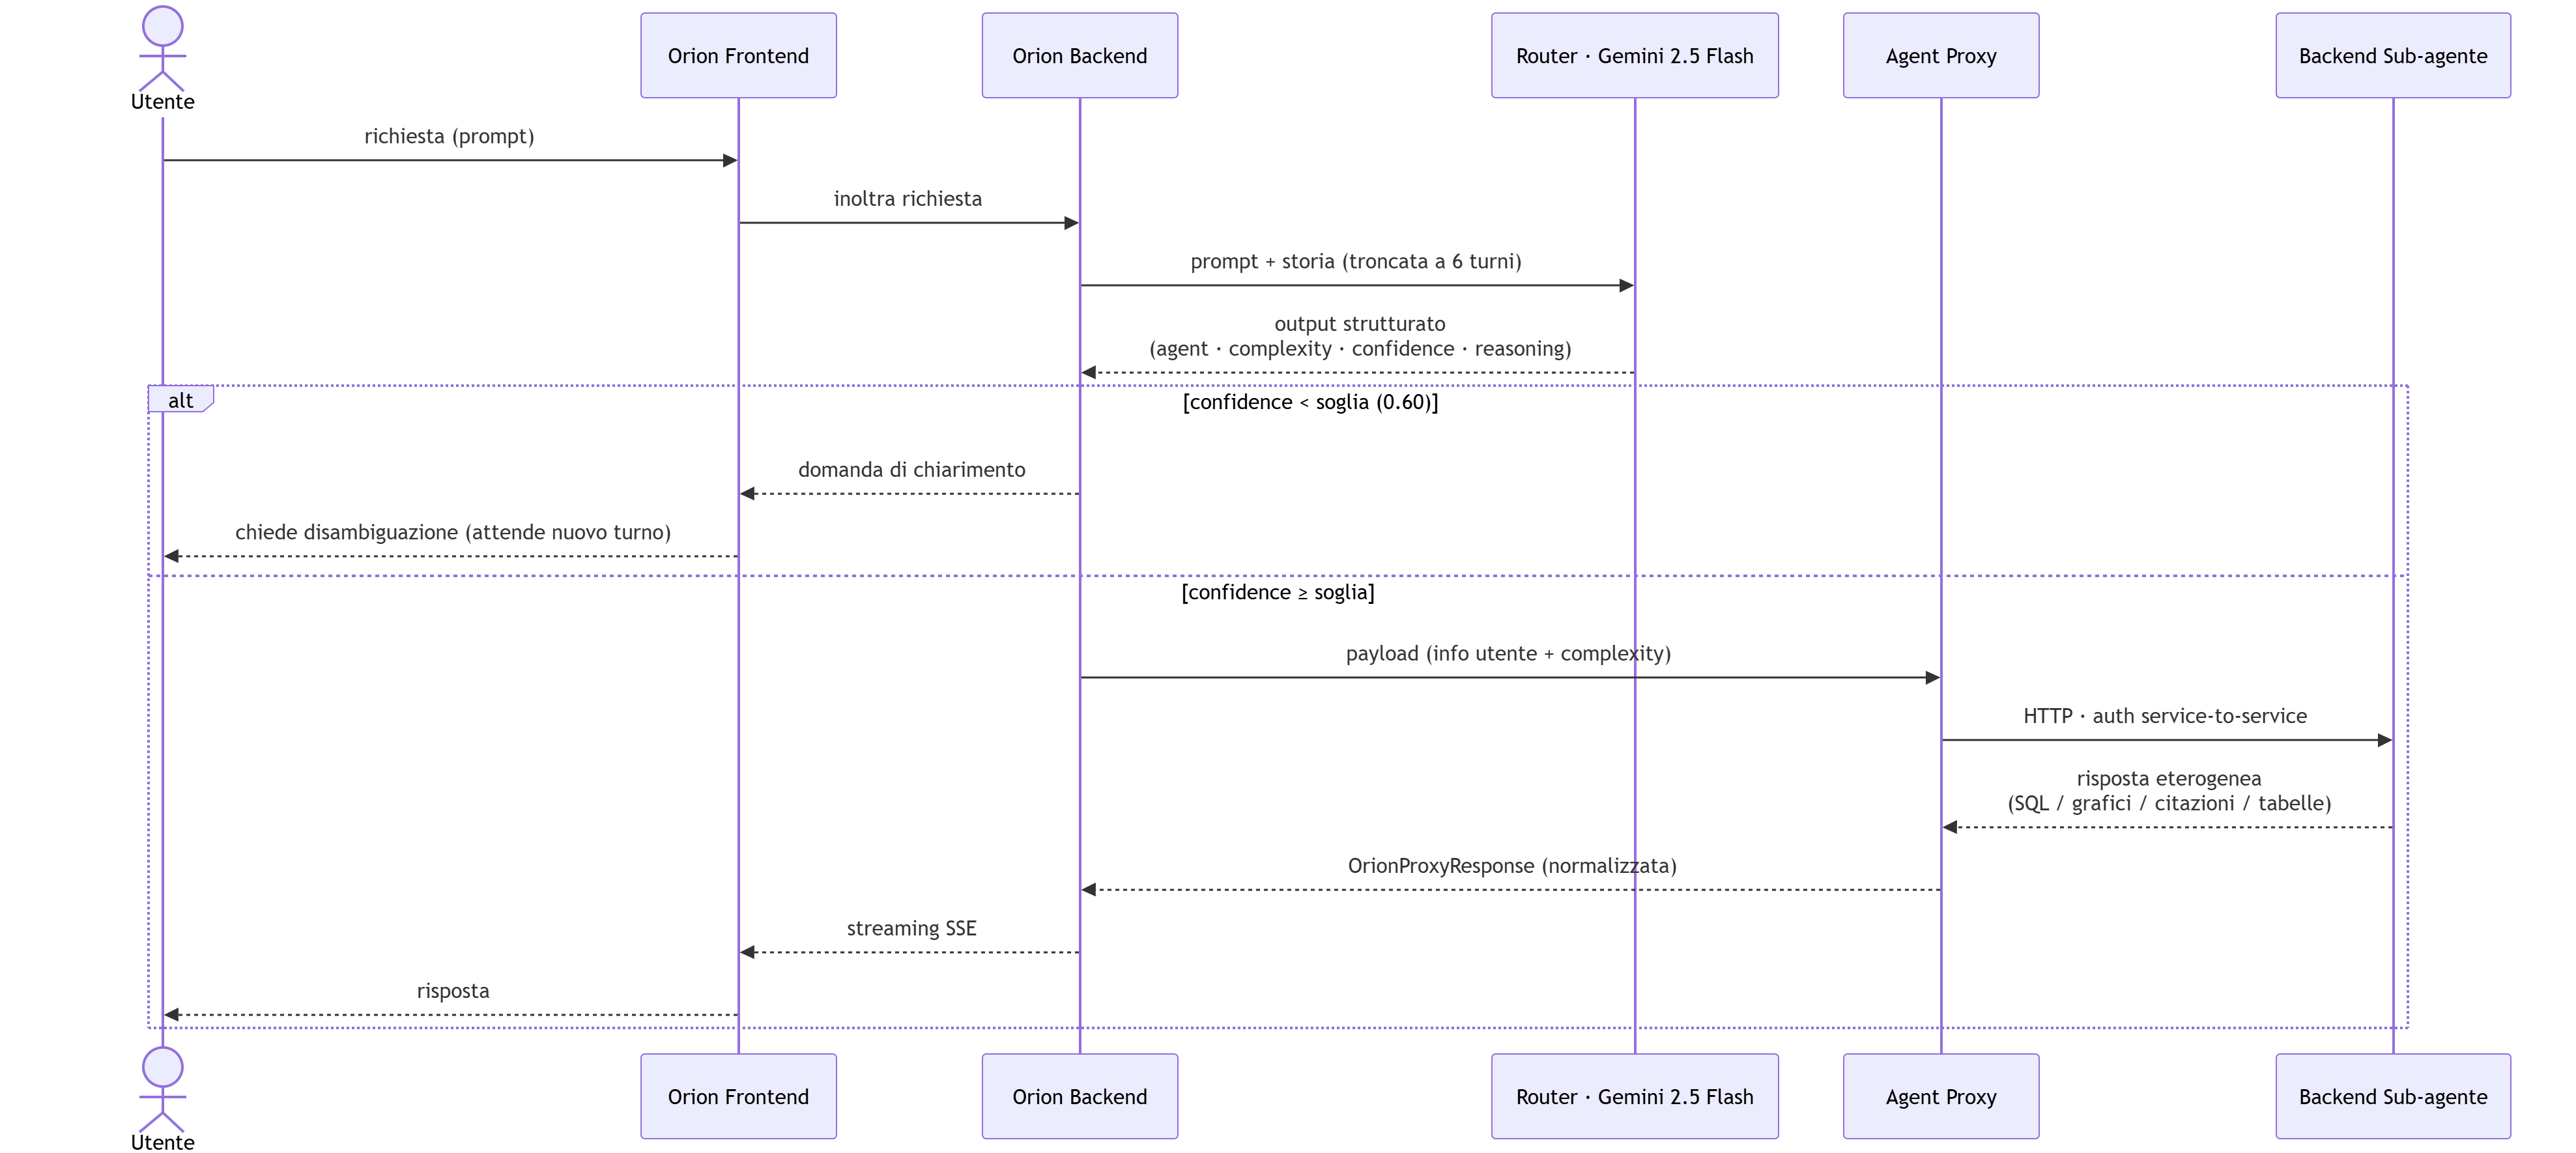
\includegraphics[width=\textwidth]{orion3}
    \caption[Sequence diagram di un turno Orion]{Sequence diagram completo: dalla richiesta utente al routing, dall'invocazione del sub-agente alla normalizzazione della risposta.}
    \label{fig:orion_sequence}
\end{figure}

% =====================================================================
\section{Conversation threading e gestione della storia}
\label{sec:orion-history}
% =====================================================================

Orion mantiene una \emph{storia unica} per conversazione: tutti i turni, indipendentemente dall'agente che li ha serviti, sono memorizzati nella stessa conversazione del database di Orion.
Questa scelta consente all'utente di cambiare argomento (e quindi agente) all'interno
della stessa conversazione senza discontinuità percepita.

Il trade-off accettato è che il sub-agente invocato riceve l'intera storia della conversazione,
inclusi i turni gestiti da altri agenti. Per mitigare il rischio di confusione, la storia inviata al sub-agente
è troncata agli ultimi sei turni (parametro configurabile) e i messaggi non pertinenti (ad esempio, grafici base64 o citazioni di documenti)
sono sostituiti con un riassunto testuale sintetico. Il router stesso riceve la storia per
migliorare la classificazione dei turni di follow-up: se l'utente ha appena chiesto informazioni sui ticket IT,
una domanda successiva come ``E quanti ne sono stati chiusi?'' viene correttamente instradata a SysAid anche in assenza di parole chiave esplicite.

% =====================================================================
\section{Integrazione nel flusso di chat e sicurezza}
\label{subsec:orion-impl-chat}
% =====================================================================

L'endpoint SSE \texttt{/api/orion/chat/stream} è il punto di ingresso per le richieste dell'utente.
Il flusso, rispetto a Vera, aggiunge un passo di routing dopo i controlli di quota e di sicurezza e prima della generazione:

\begin{enumerate}
  \item Verifica quota token dell'utente.
  \item Sanitizzazione del prompt (Model Armor).
  \item \textbf{[Nuovo]} Chiamata a \texttt{router\_agent.classify()}.
  \item \textbf{[Nuovo]} Logging della decisione in \texttt{orion\_routing\_logs}.
  \item Se \texttt{clarification\_needed}: ritorno della domanda all'utente, fine del turno.
  \item Se \texttt{agent != "self"}: chiamata a \texttt{agent\_proxy.forward()}, ritorno della risposta normalizzata.
  \item Se \texttt{agent == "self"} e la conversazione ha documenti caricati: pipeline RAG interna (Gemini Context Caching).
  \item Se \texttt{agent == "self"} senza documenti: pipeline generalista (ricerca web, conoscenza parametrica, streaming SSE).
\end{enumerate}

La Fig.~\ref{fig:security_chain_orion} visualizza il flusso completo come evoluzione della
catena di sicurezza di Vera (Fig.~\ref{fig:security_chain}): il \emph{routing step} si innesta fra il
controllo di sicurezza sul prompt e la generazione.
Le tre diramazioni del router riconfluiscono prima della sanitizzazione dell'output, così che ogni risposta,
inclusa quella prodotta da un sub-agente, attraversi i medesimi controlli post-generazione e lo stesso audit della pipeline originaria.

\begin{figure}[htbp]
    \centering
    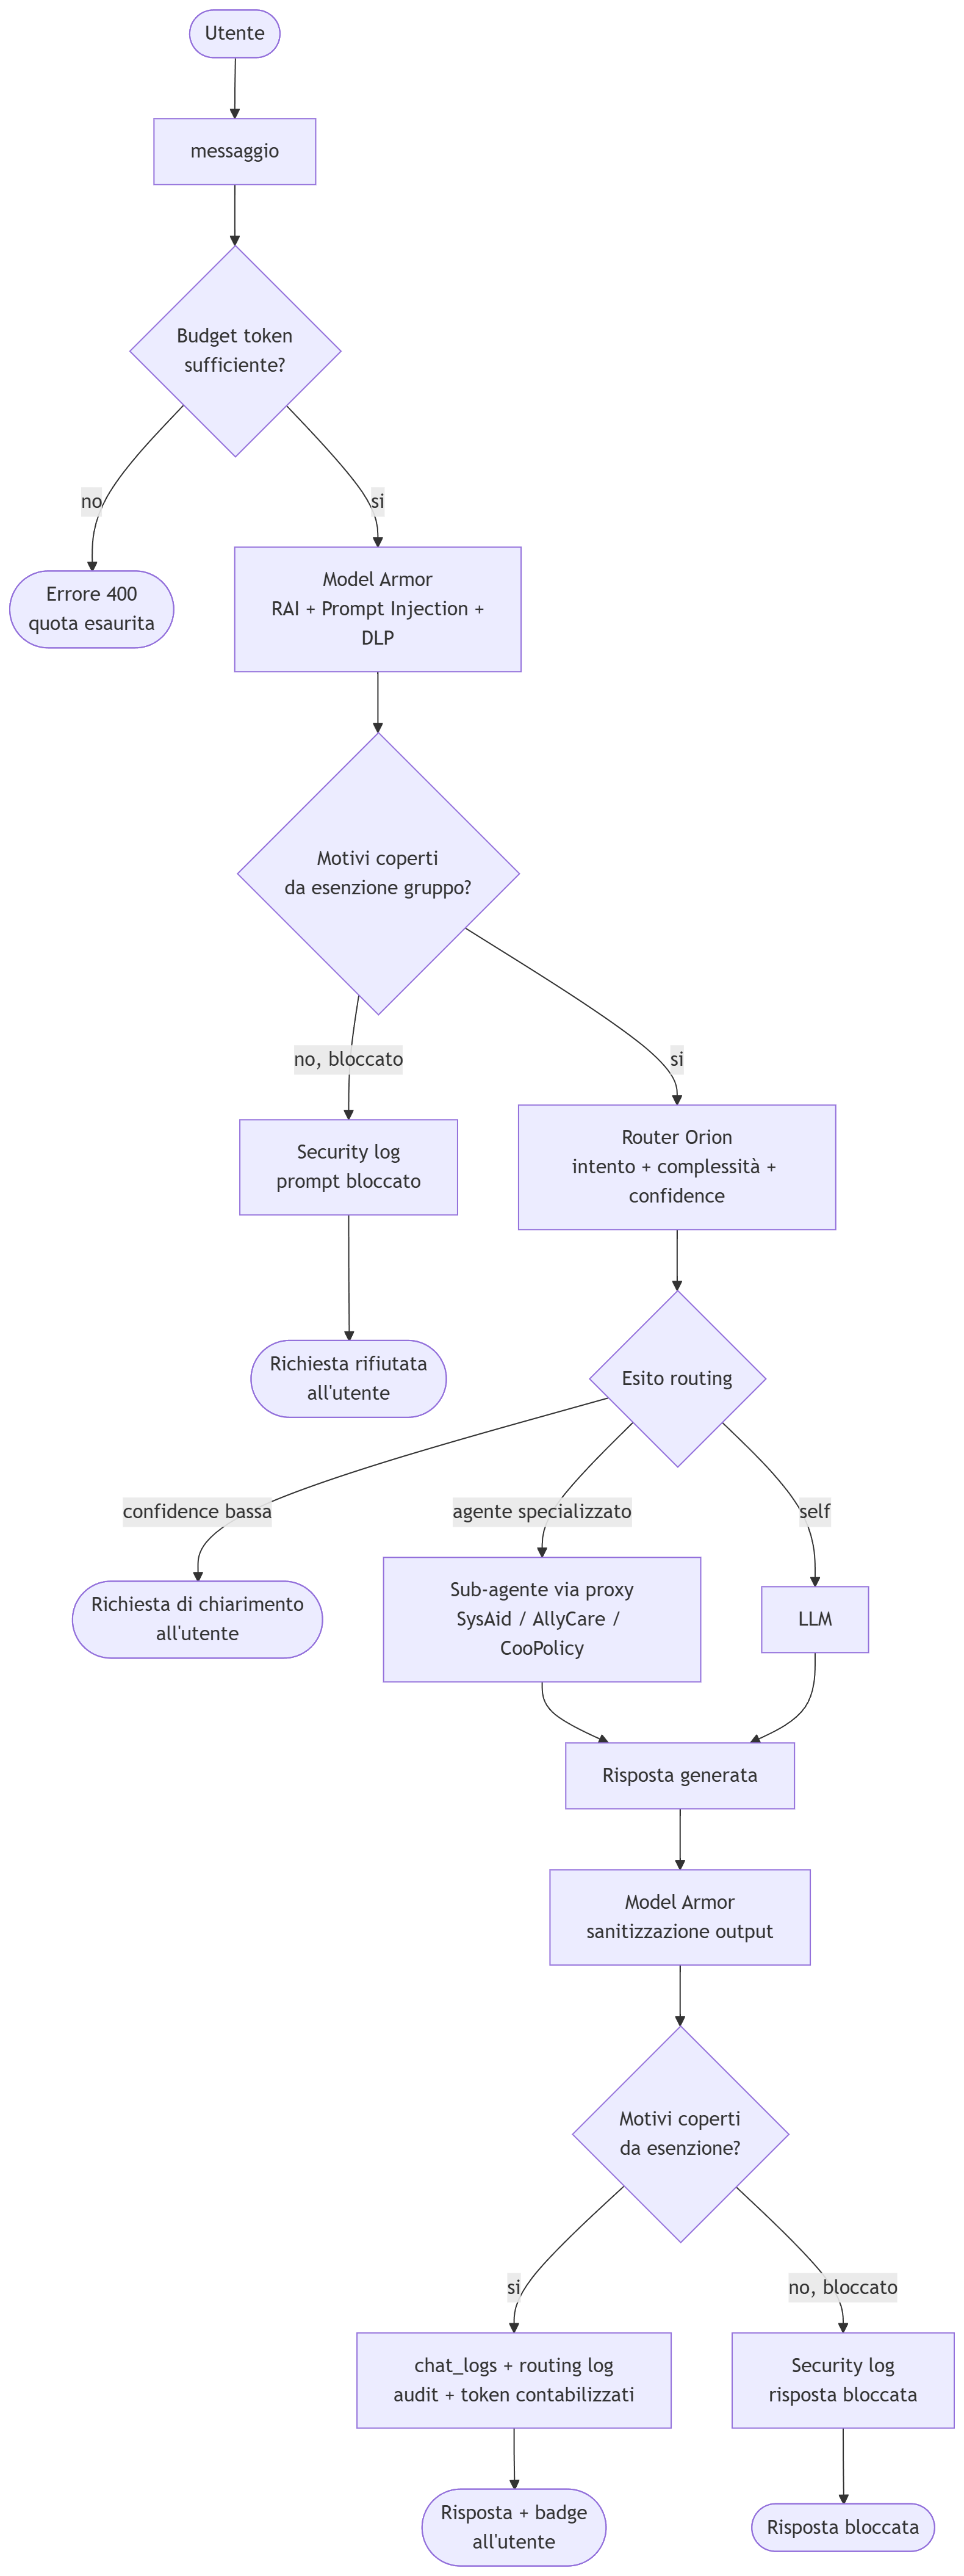
\includegraphics[width=0.95\textwidth,height=0.9\textheight,keepaspectratio]{flusso-prompt-full-orion}
    \caption[Catena di sicurezza e routing di Orion]{Il flusso completo di una richiesta in Orion: verifica della quota, sanitizzazione del prompt tramite Model Armor
    (RAI, prompt injection, DLP) con esenzioni per gruppo, \emph{routing step} che instrada verso la pipeline interna, un sub-agente specializzato oppure una richiesta di chiarimento,
    e infine sanitizzazione dell'output e audit su \texttt{chat\_logs}. Evoluzione della Fig.~\ref{fig:security_chain} con l'aggiunta dello strato di orchestrazione.}
    \label{fig:security_chain_orion}
\end{figure}

Il routing step viene eseguito \emph{sempre}, anche in presenza di documenti caricati:
ciò consente all'utente di porre, nella stessa conversazione, sia domande sui propri documenti sia richieste destinate a un sub-agente.
La selezione tra la pipeline RAG interna e la pipeline generalista avviene \emph{dopo} il routing, sulla base del campo \texttt{agent} restituito dal router.

% =====================================================================
\section{Frontend}
\label{sec:orion-impl-frontend}
% =====================================================================

Il frontend di Orion è un'applicazione React~19 con TypeScript, derivata dal frontend di Vera e
adattata per la nuova architettura. Le differenze significative riguardano tre aspetti:
il rendering del badge di routing, la gestione delle \emph{response shape} eterogenee e il supporto alle citazioni di CooPolicy.

\subsection{Badge di routing e trasparenza}
\label{subsec:orion-impl-fe-routing}

Ogni messaggio di risposta include un \emph{badge} visibile sopra il testo che
indica quale agente ha servito la richiesta e con quale livello di complessità:
ad esempio, ``SysAid $\cdot$ Alta'' o ``CooPolicy $\cdot$ Bassa''.
Il badge è un componente React che riceve i campi \texttt{agent\_used} e \texttt{complexity}
dall'oggetto \texttt{OrionProxyResponse}. La scelta di rendere visibile il routing è motivata da due ragioni: il valore dimostrativo nel contesto della tesi,
e la fiducia dell'utente nel sistema (l'utente vede che la risposta proviene da un agente specializzato).

\begin{figure}[htbp]
  \centering
  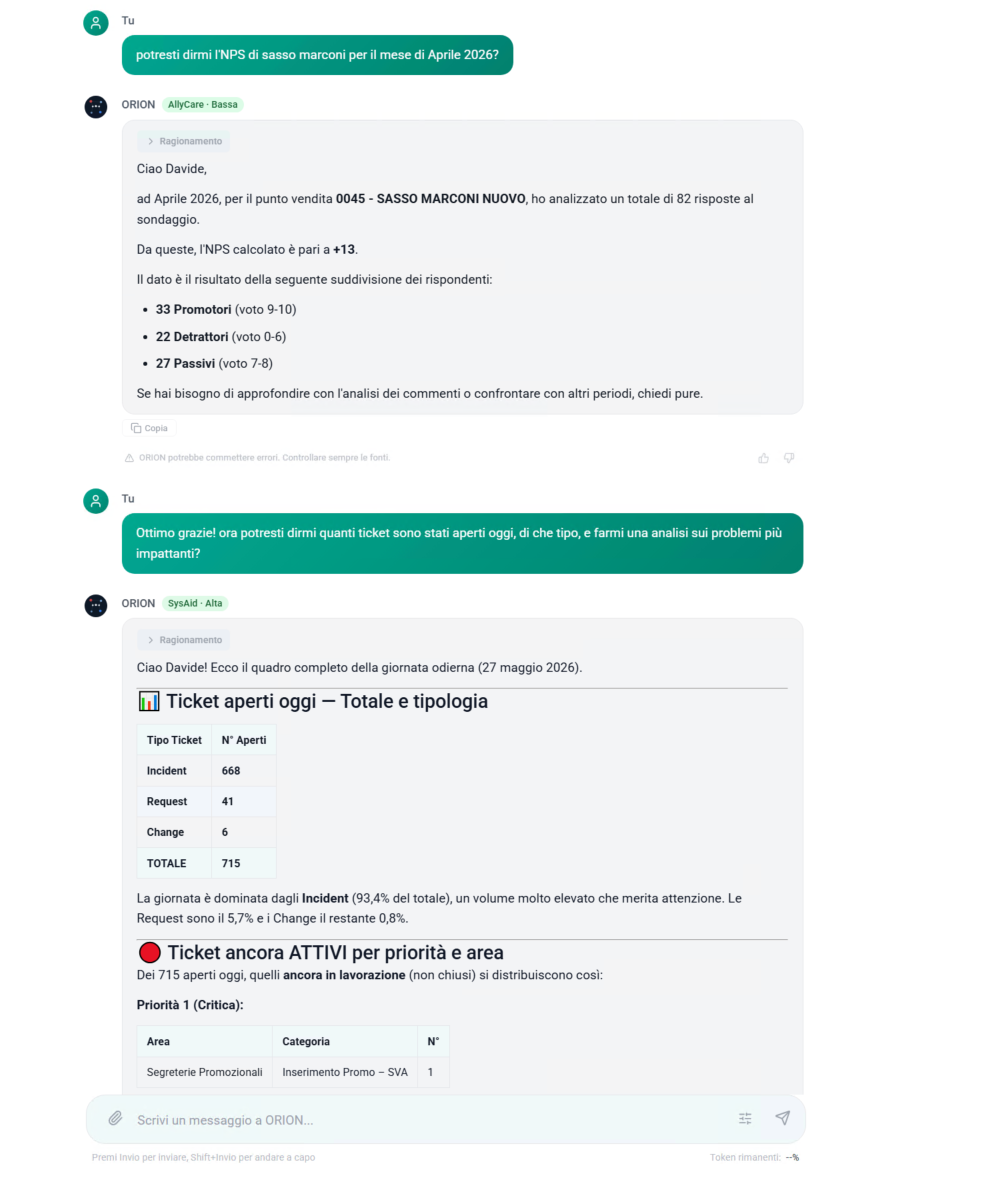
\includegraphics[width=0.7\textwidth,height=0.9\textheight,keepaspectratio]{routing1}
  \caption[Orion: cambio agente nella stessa conversazione]{Routing trasparente con cambio di agente all'interno di un'unica conversazione: la prima richiesta (NPS) è instradata ad AllyCare (badge \emph{ORION $\cdot$ AllyCare $\cdot$ Bassa}), la successiva (ticket IT) a SysAid (badge \emph{ORION $\cdot$ SysAid $\cdot$ Alta}), senza che l'utente debba cambiare strumento.}
  \label{fig:orion_switch}
\end{figure}

\begin{figure}[htbp]
  \centering
  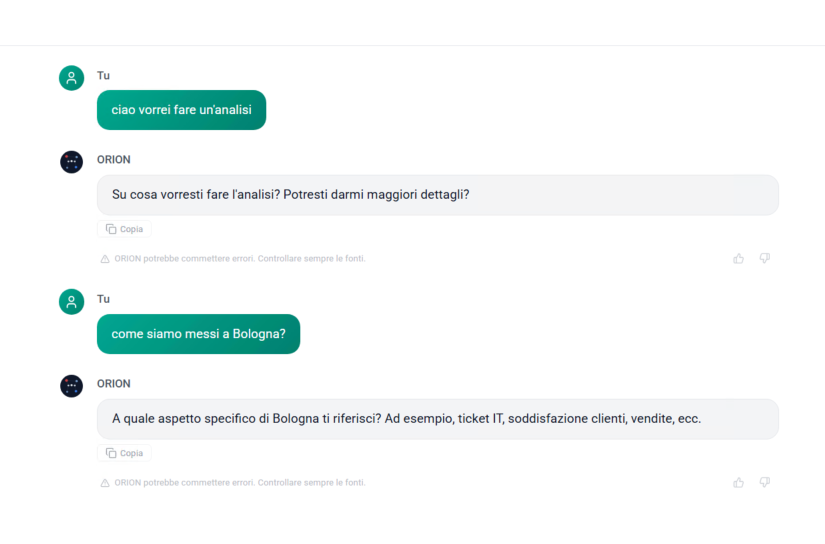
\includegraphics[width=0.95\textwidth,keepaspectratio]{approfondimenti-routing}
  \caption[Orion: meccanismo di clarification]{Il meccanismo di \emph{clarification}: quando la confidence del router è sotto la soglia, Orion non instrada ma pone all'utente una domanda di disambiguazione (``Su cosa vorresti fare l'analisi?'', ``A quale aspetto di Bologna ti riferisci?'') prima di procedere.}
  \label{fig:orion_clarification}
\end{figure}

\subsection{Renderer adattivo per risposte eterogenee}
\label{subsec:orion-impl-fe-shapes}

Il frontend implementa un renderer che si adatta
alla \emph{shape} della risposta in base al campo \texttt{agent\_used}:

\begin{itemize}
  \item \textbf{SysAid / AllyCare:} la risposta può includere grafici (\texttt{charts}:
  array di immagini base64), tabelle dati (\texttt{data}: JSON) e
  query SQL (\texttt{queries}: array di stringhe). I grafici vengono renderizzati in coda alla risposta,
  i dati in una tabella espandibile con download CSV, le query in un blocco codice collassabile.
  \item \textbf{CooPolicy:} la risposta include citazioni (\texttt{sources}: array con titolo, snippet, URI normalizzata).
  Le citazioni sono rese come link cliccabili che aprono il PDF originale attraverso il proxy \texttt{/api/orion/docs/file}.
  Le tabelle Markdown eventualmente presenti nella risposta sono renderizzate con \texttt{remark-gfm}.
  \item \textbf{Self (Orion):} la risposta segue il formato di Vera, con citazioni web inline e supporto a documenti caricati.
\end{itemize}

\begin{figure}[htbp]
  \centering
  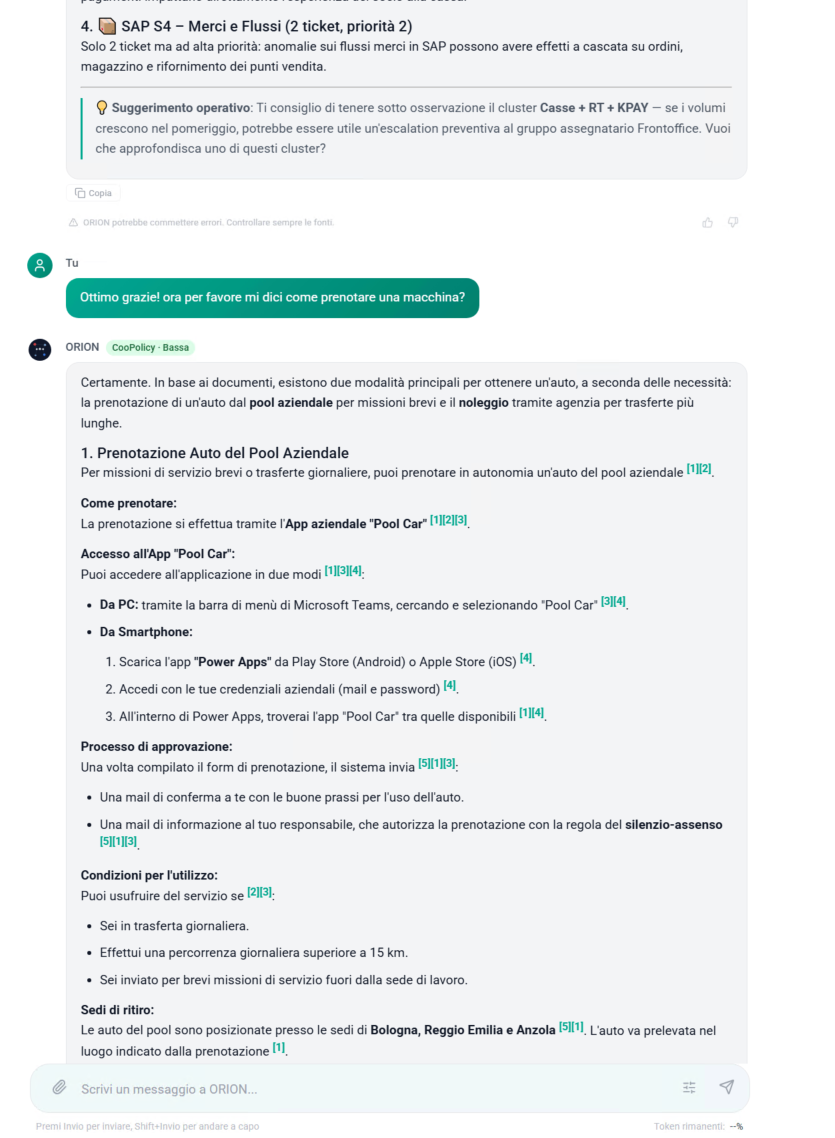
\includegraphics[width=0.65\textwidth,height=0.9\textheight,keepaspectratio]{routing3}
  \caption[Orion: instradamento a CooPolicy con citazioni]{Una richiesta su una policy aziendale instradata a CooPolicy attraverso Orion: la risposta conserva le citazioni numerate \texttt{[N]} ai documenti sorgente, normalizzate dal proxy e rese cliccabili dal frontend.}
  \label{fig:orion_coopolicy}
\end{figure}

% =====================================================================
\section{Admin Panel di Orion}
\label{sec:orion-impl-admin}
% =====================================================================

Il pannello di amministrazione di Orion è composto da un frontend React
(\texttt{orion-admin-frontend}) e da un backend FastAPI dedicato
(\texttt{orion-admin-backend}), accessibili dal portale amministrativo.
In continuità architetturale con Vera, che dispone della coppia
\texttt{vera-admin-backend} / \texttt{vera-admin-frontend},
il backend admin di Orion è un servizio Cloud Run separato dal backend
principale, derivato dalla stessa base di \texttt{vera-admin-backend} e
operante sulle tabelle \texttt{orion\_*} del database condiviso.
I suoi endpoint sono serviti sotto il prefisso \texttt{/api/orion-admin/}.

Il pannello condivide con quello di Vera (Sez.~\ref{sec:agenti-admin-impl})
le pagine di gestione standard --- budget token, statistiche di consumo,
log conversazioni, feedback strutturato, esenzioni PII, impostazioni Model
Armor --- e aggiunge le sezioni specifiche per l'orchestratore:

\begin{description}
  \item[Routing Logs.] Tabella paginata delle decisioni di routing, con timestamp, username, estratto del prompt,
  agente selezionato, complessità, confidence (con codifica cromatica: verde $\geq 0{,}80$, giallo $\geq 0{,}60$, rosso $< 0{,}60$), flag di clarification. Il click su una riga espande il \emph{reasoning} completo del router, consentendo all'amministratore di diagnosticare le classificazioni errate.

  \item[Router Prompt.] Editor del \emph{system prompt} del router con textarea a tutta larghezza,
  indicazione della data dell'ultimo aggiornamento e bottone ``Salva e Attiva''.
  Il prompt è persistito nella tabella \texttt{app\_settings} del database, non nel codice:
  questo consente di iterare il prompt senza un nuovo rilascio del backend.

  \item[Metriche di Routing.] Dashboard con quattro KPI (richieste totali, confidence media, clarification rate, numero di agenti attivi)
  e un grafico a barre della distribuzione delle richieste per agente.

  \item[Eval Routing.] Pagina di valutazione automatica del routing: consente
  di gestire la test suite, lanciare run di valutazione e confrontare lo
  storico delle run direttamente dal browser. È lo strumento con cui è stata
  condotta la valutazione sperimentale di questa tesi, ed è descritta in
  dettaglio nel Capitolo~\ref{chap:orion-valutazione}
  (Sez.~\ref{subsec:eval-admin-page}).
\end{description}

% =====================================================================
\section{Infrastruttura e persistenza}
\label{sec:orion-impl-iac}
% =====================================================================
\label{sec:orion-impl-db}

L'infrastruttura di Orion aggiunge i quattro servizi Cloud Run citati al deployment Terraform esistente.
Ciascun servizio ha il proprio trigger Cloud Build collegato al rispettivo repository Bitbucket.
Le variabili d'ambiente specifiche di Orion (URL dei sub-agenti, soglia di confidence, modello del router)
sono iniettate da Terraform attraverso il file \texttt{tfvars} dell'ambiente corrispondente, seguendo lo stesso pattern
degli altri servizi della suite (Sez.~\ref{subsec:agenti-iac}).

Il database di Orion è ospitato sulla stessa istanza Cloud SQL della suite (database \texttt{ai\_agents\_db}),
con tabelle distinte identificate dal prefisso \texttt{orion\_}. Le tabelle principali sono:

\begin{itemize}
  \item \texttt{orion\_users}, \texttt{orion\_conversations}, \texttt{orion\_messages}: ereditate dalla struttura di Vera, gestiscono utenti, conversazioni e messaggi.
  \item \texttt{orion\_routing\_logs}: registra ogni decisione del router con username, estratto del prompt, agente selezionato, complessità, confidence, flag di clarification e reasoning completo.
  \item \texttt{orion\_eval\_test\_cases}: contiene i test case della suite di valutazione (ID, prompt, agente atteso, complessità attesa, categoria, note).
  \item \texttt{orion\_eval\_results}: contiene i risultati di ogni run di valutazione (run ID, versione del prompt, agente atteso vs prodotto, complessità attesa vs prodotta, confidence, reasoning, flag di correttezza).
\end{itemize}

Come per il resto della suite (Cap.~\ref{chap:agenti}), non si utilizzano
framework di migrazione: tutte le tabelle sono create automaticamente e in
modo idempotente al primo avvio di ciascun servizio tramite
\texttt{Base.metadata.create\_all()} (il primo servizio che parte crea lo
schema, il secondo lo trova già presente), e le eventuali evoluzioni dello
schema sono gestite con istruzioni \texttt{ALTER TABLE ... ADD COLUMN IF NOT
EXISTS} nel codice di inizializzazione.

\begin{figure}[htbp]
    \centering
    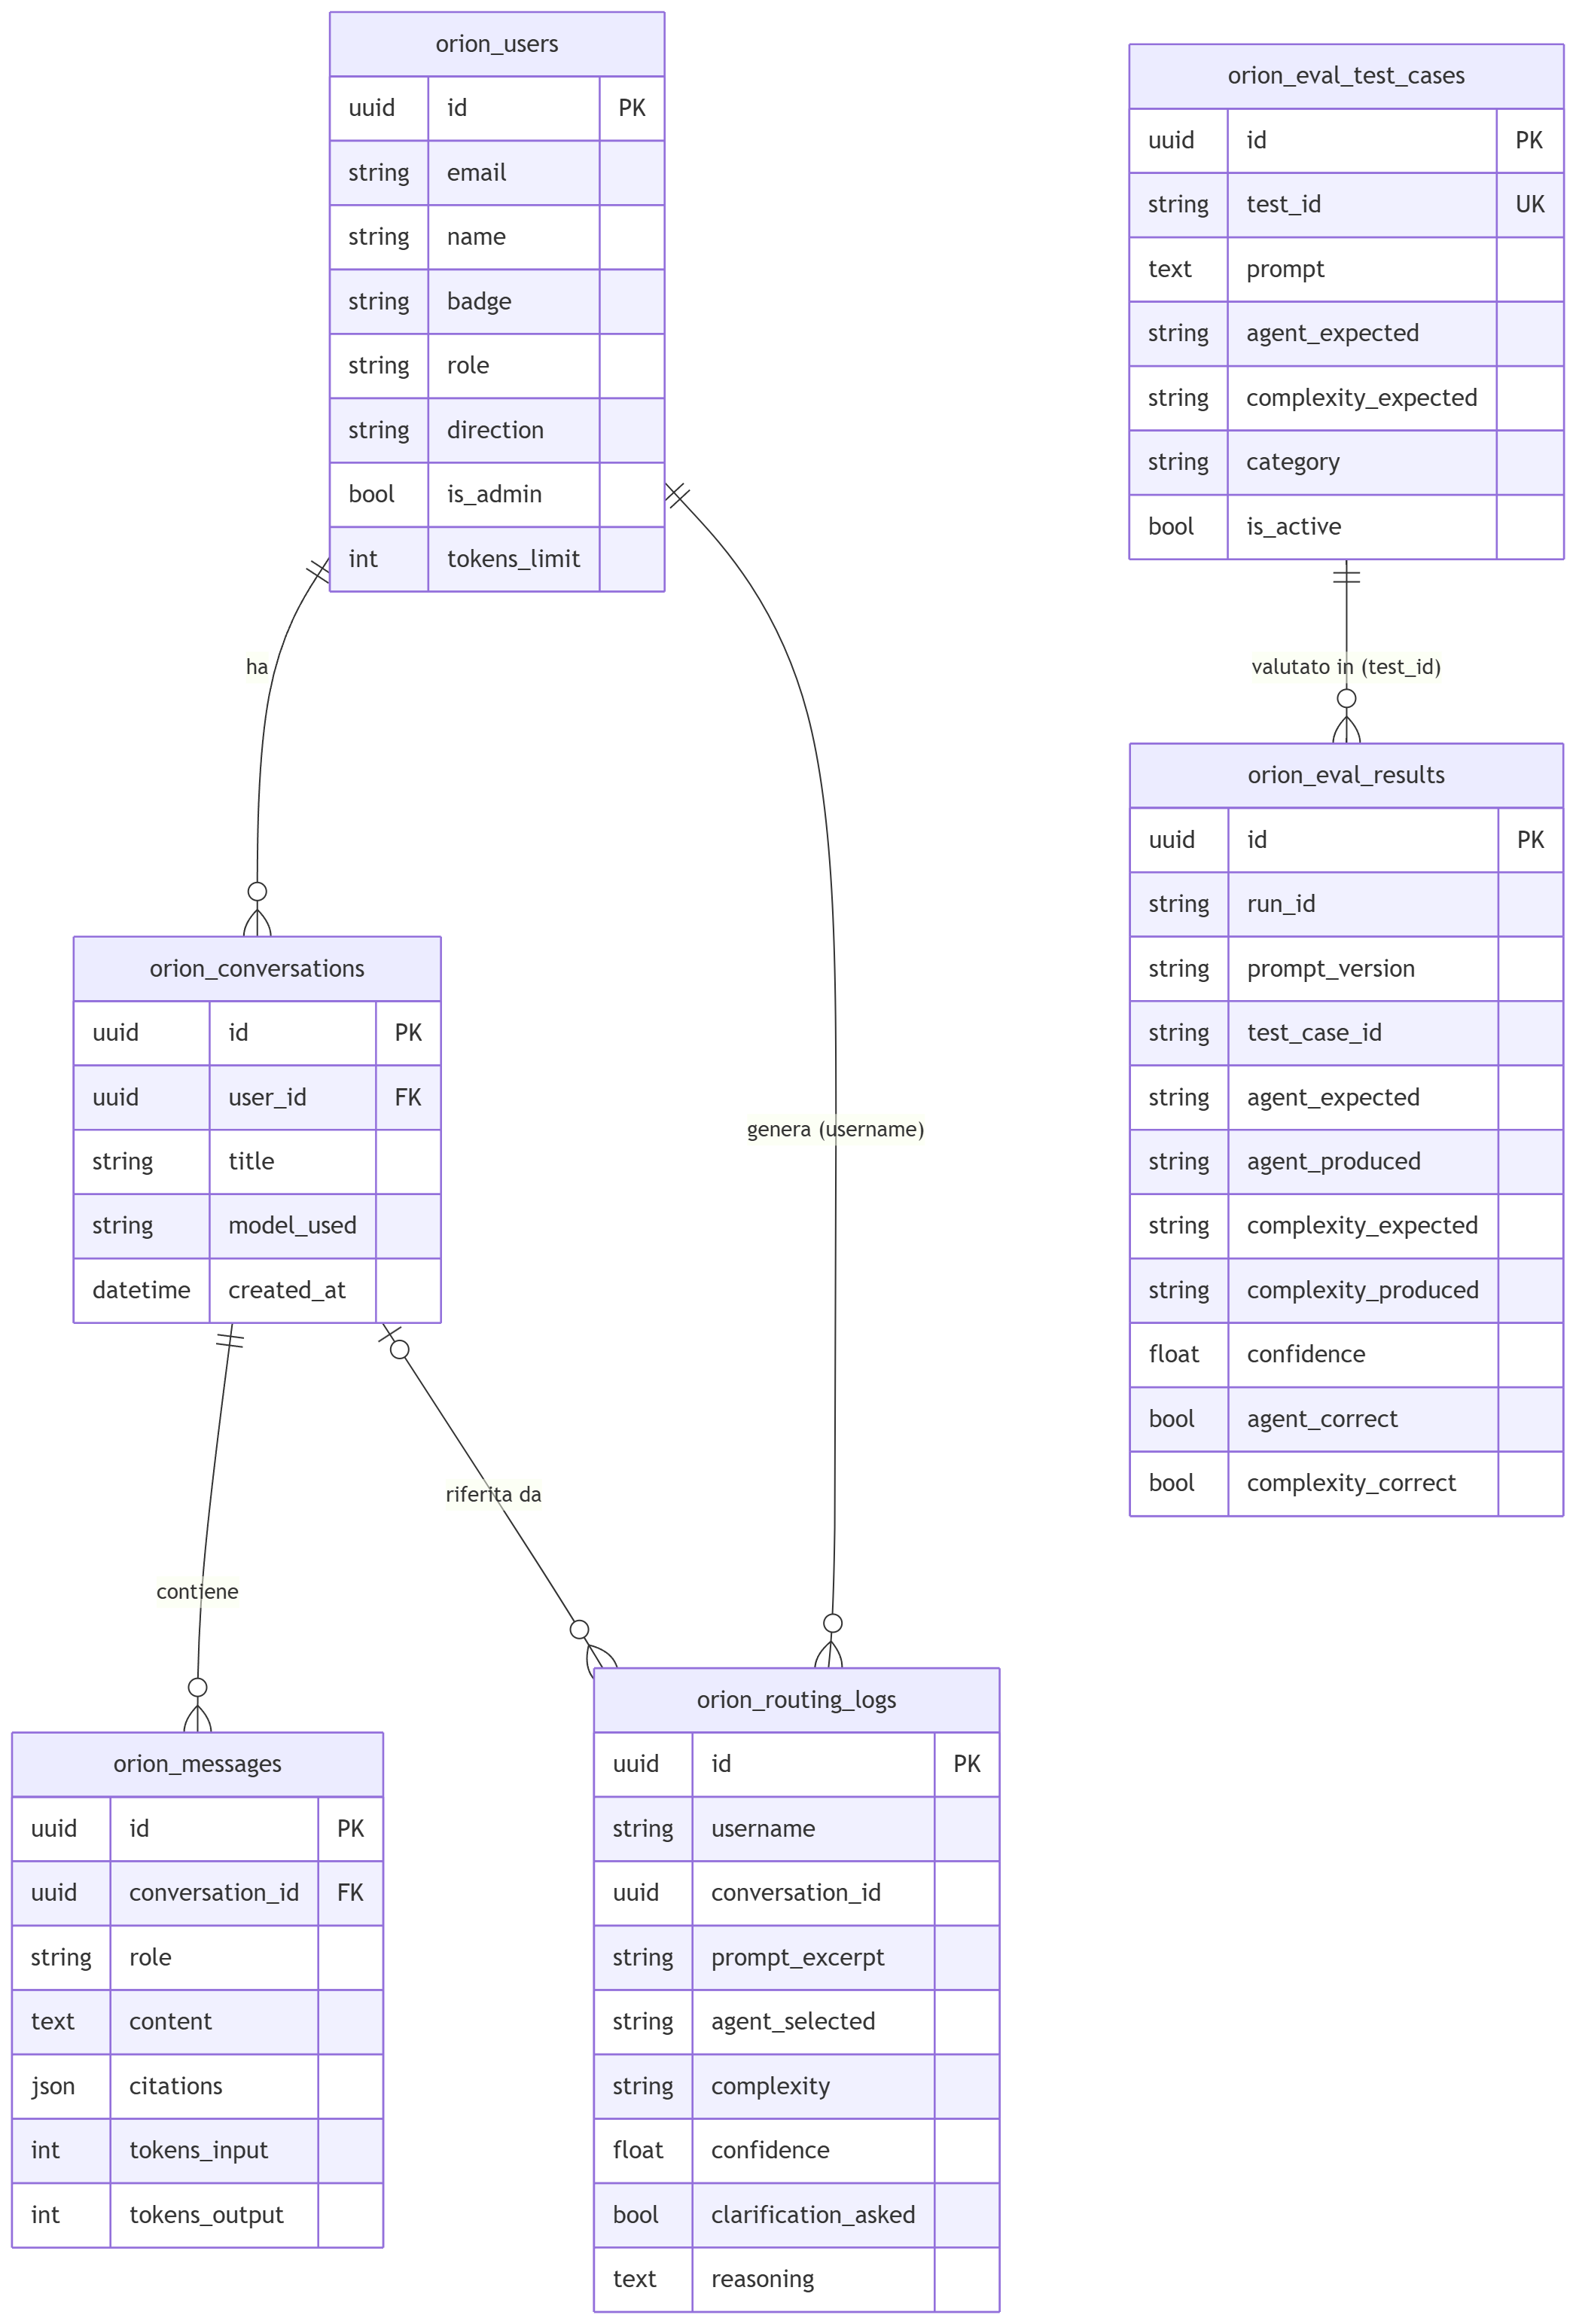
\includegraphics[height=0.9\textheight,keepaspectratio]{orion-er}
    \caption[Schema del database Orion]{Schema relazionale del database di Orion: utenti, conversazioni, messaggi, log di routing e tabelle di valutazione (colonne tratte dai modelli SQLAlchemy del backend).}
    \label{fig:orion_er}
\end{figure}

% =====================================================================
\section{Decisioni architetturali e loro motivazione}
\label{sec:orion-decisioni}
% =====================================================================

Questa sezione riassume le principali decisioni architetturali di Orion,
documentando per ciascuna le alternative considerate e le ragioni della scelta effettuata.

\begin{table}[htbp]
  \centering
  \caption[Decisioni architetturali di Orion]{Principali decisioni architetturali di Orion con alternative considerate e motivazione della scelta.}
  \label{tab:orion-decisioni}
  \begin{tabular}{p{3.5cm}p{3.5cm}p{6cm}}
    \toprule
    \textbf{Decisione}       & \textbf{Alternativa}        & \textbf{Motivazione}                   \\
    \midrule
    Modello routing: Gemini Flash
                             & Gemini Pro, Claude, router appreso~\cite{ong2024routellm}
                             & Latenza sub-secondo, costo trascurabile, capacità sufficiente per classificazione a $K$ etichette \\
    Soglia confidence: 0,60  & 0,50, 0,70, adattiva
                             & Compromesso tra clarification rate e accuracy, calibrato empiricamente (Cap.~\ref{chap:orion-valutazione}) \\
    Storia: unica in Orion   & Separata per agente
                             & Continuità dell'esperienza utente; i sub-agenti ricevono storia troncata \\
    Routing trasparente      & Nascosto
                             & Badge visibile sopra la risposta con agente e complessità; valore dimostrativo e fiducia utente \\
    \bottomrule
  \end{tabular}
\end{table}

% !TEX root = ../main.tex
% =====================================================================
% CAPITOLO 5 — VALUTAZIONE SPERIMENTALE
% (ex capitolo 7; in espansione su richiesta dei relatori — vedi
%  plans/PIANO_REVISIONE_FEEDBACK.md, attività F2)
% =====================================================================

\chapter{Valutazione sperimentale}
\label{chap:orion-valutazione}

Questo capitolo presenta la valutazione sperimentale del sistema su quattro piani complementari.
Il primo, e più esteso, è il terzo contributo della tesi: una metodologia di valutazione del routing di Orion tramite uno strumento di esecuzione automatica integrato nell'admin panel,
progettata per misurare in modo sistematico e ripetibile l'accuratezza delle decisioni dell'orchestratore e per guidare il miglioramento del \emph{system prompt} del router.
L'oggetto di questa iterazione --- il prompt stesso, con le tecniche di prompt engineering che incorpora --- è esaminato nella Sez.~\ref{sec:eval-prompteng};
i risultati su due versioni successive del prompt (v1.0 e v1.1) ne illustrano sia l'utilità sia i limiti.

Il secondo piano (Sez.~\ref{sec:eval-agenti}) valuta la \emph{qualità dei sub-agenti}: execution accuracy per gli agenti Text-to-SQL e faithfulness per il RAG,
applicando le metodologie introdotte nel background (Sez.~\ref{subsec:bg-text2sql} e~\ref{sec:bg-ragas}).

Il terzo piano (Sez.~\ref{sec:eval-costo-qualita}) analizza il trade-off costo--qualità realizzato dal routing per complessità,
chiudendo il percorso aperto nel background (Sez.~\ref{sec:bg-routing}); il quarto (Sez.~\ref{sec:eval-costi}) propone una valutazione economica indicativa
del costo di implementazione del progetto rispetto all'adozione di licenze SaaS.
Chiude il capitolo la discussione complessiva dei risultati e dei limiti dell'impianto sperimentale (Sez.~\ref{sec:eval-discussione}).

% =====================================================================
\section{Domande di ricerca}
\label{sec:eval-research-questions}
% =====================================================================

La valutazione è guidata da sei domande di ricerca:

\begin{description}
  \item[RQ1] Quanto è accurato il routing dell'orchestratore? (\emph{Agent Accuracy})
  \item[RQ2] Quanto è accurata la stima di complessità? (\emph{Complexity Accuracy})
  \item[RQ3] Il confidence score è calibrato? È più alto sui casi corretti che su quelli errati?
  \item[RQ4] Il meccanismo di clarification riduce l'errore senza degradare l'esperienza utente?
  \item[RQ5] Iterazioni successive del system prompt migliorano le metriche in modo misurabile?
  \item[RQ6] Il routing per complessità preserva la qualità delle risposte riducendo il costo? (\emph{costo--qualità})
\end{description}

La metodologia adottata combina elementi dell'approccio \emph{AgentBench}~\cite{liu2023agentbench}
per la valutazione di agenti LLM con il paradigma del prompt engineering iterativo~\cite{sahoo2024prompteng_survey}:
un gold standard fisso, un'esecuzione automatica, metriche dichiarate a priori, iterazione controllata del prompt con confronto quantitativo.

% =====================================================================
\section{Metodologia di valutazione}
\label{sec:eval-metodologia}
% =====================================================================

\subsection{Costruzione del gold standard}
\label{subsec:eval-gold-standard}

La test suite è composta da 120 test case, ciascuno definito da un prompt in linguaggio naturale, 
un agente atteso (\texttt{self}, \texttt{sysaid}, \texttt{allycare}, \texttt{coopolicy}), una complessità attesa (\texttt{low} o \texttt{high}) e una categoria tematica.

La costruzione è avvenuta in tre fasi:

\begin{enumerate}
  \item \textbf{Campionamento da log reali.} I prompt più frequenti nelle conversazioni di ciascun agente (raccolti durante la fase di test della suite) 
  sono stati anonimizzati e riformulati per eliminare riferimenti personali. 
  Questa fase ha prodotto circa 80~prompt rappresentativi del traffico effettivo.

  \item \textbf{Prompt sintetici per casi limite.} Sono stati creati manualmente circa 30~prompt progettati per esplorare le zone di ambiguità: 
  sovrapposizioni tra SysAid e AllyCare, tra Orion e CooPolicy (domande che potrebbero essere sia generiche sia documentali), 
  e richieste deliberatamente fuori dominio.

  \item \textbf{Prompt di sicurezza.} Un sottoinsieme di 10~prompt testa il comportamento del router su richieste malevole (prompt injection, richieste di dati personali) 
  per verificare che vengano gestite dalla pipeline di sicurezza.
\end{enumerate}

Le categorie tematiche sono cinque: \emph{SysAid} (36~casi), \emph{NPS} (21~casi), \emph{Policy} (33~casi), \emph{General} (23~casi) e \emph{Ambiguous} (7~casi).
La distribuzione riflette approssimativamente il volume di traffico atteso, con un \emph{oversampling} deliberato della categoria \emph{Ambiguous} per testare il meccanismo di clarification.

I test case sono raccolti in un file CSV (\texttt{test\_suite\_orion.csv}) e importati nel database dell'admin panel attraverso la pagina \emph{Eval Routing} (Sez.~\ref{subsec:eval-admin-page}).

\begin{figure}[htbp]
    \centering
    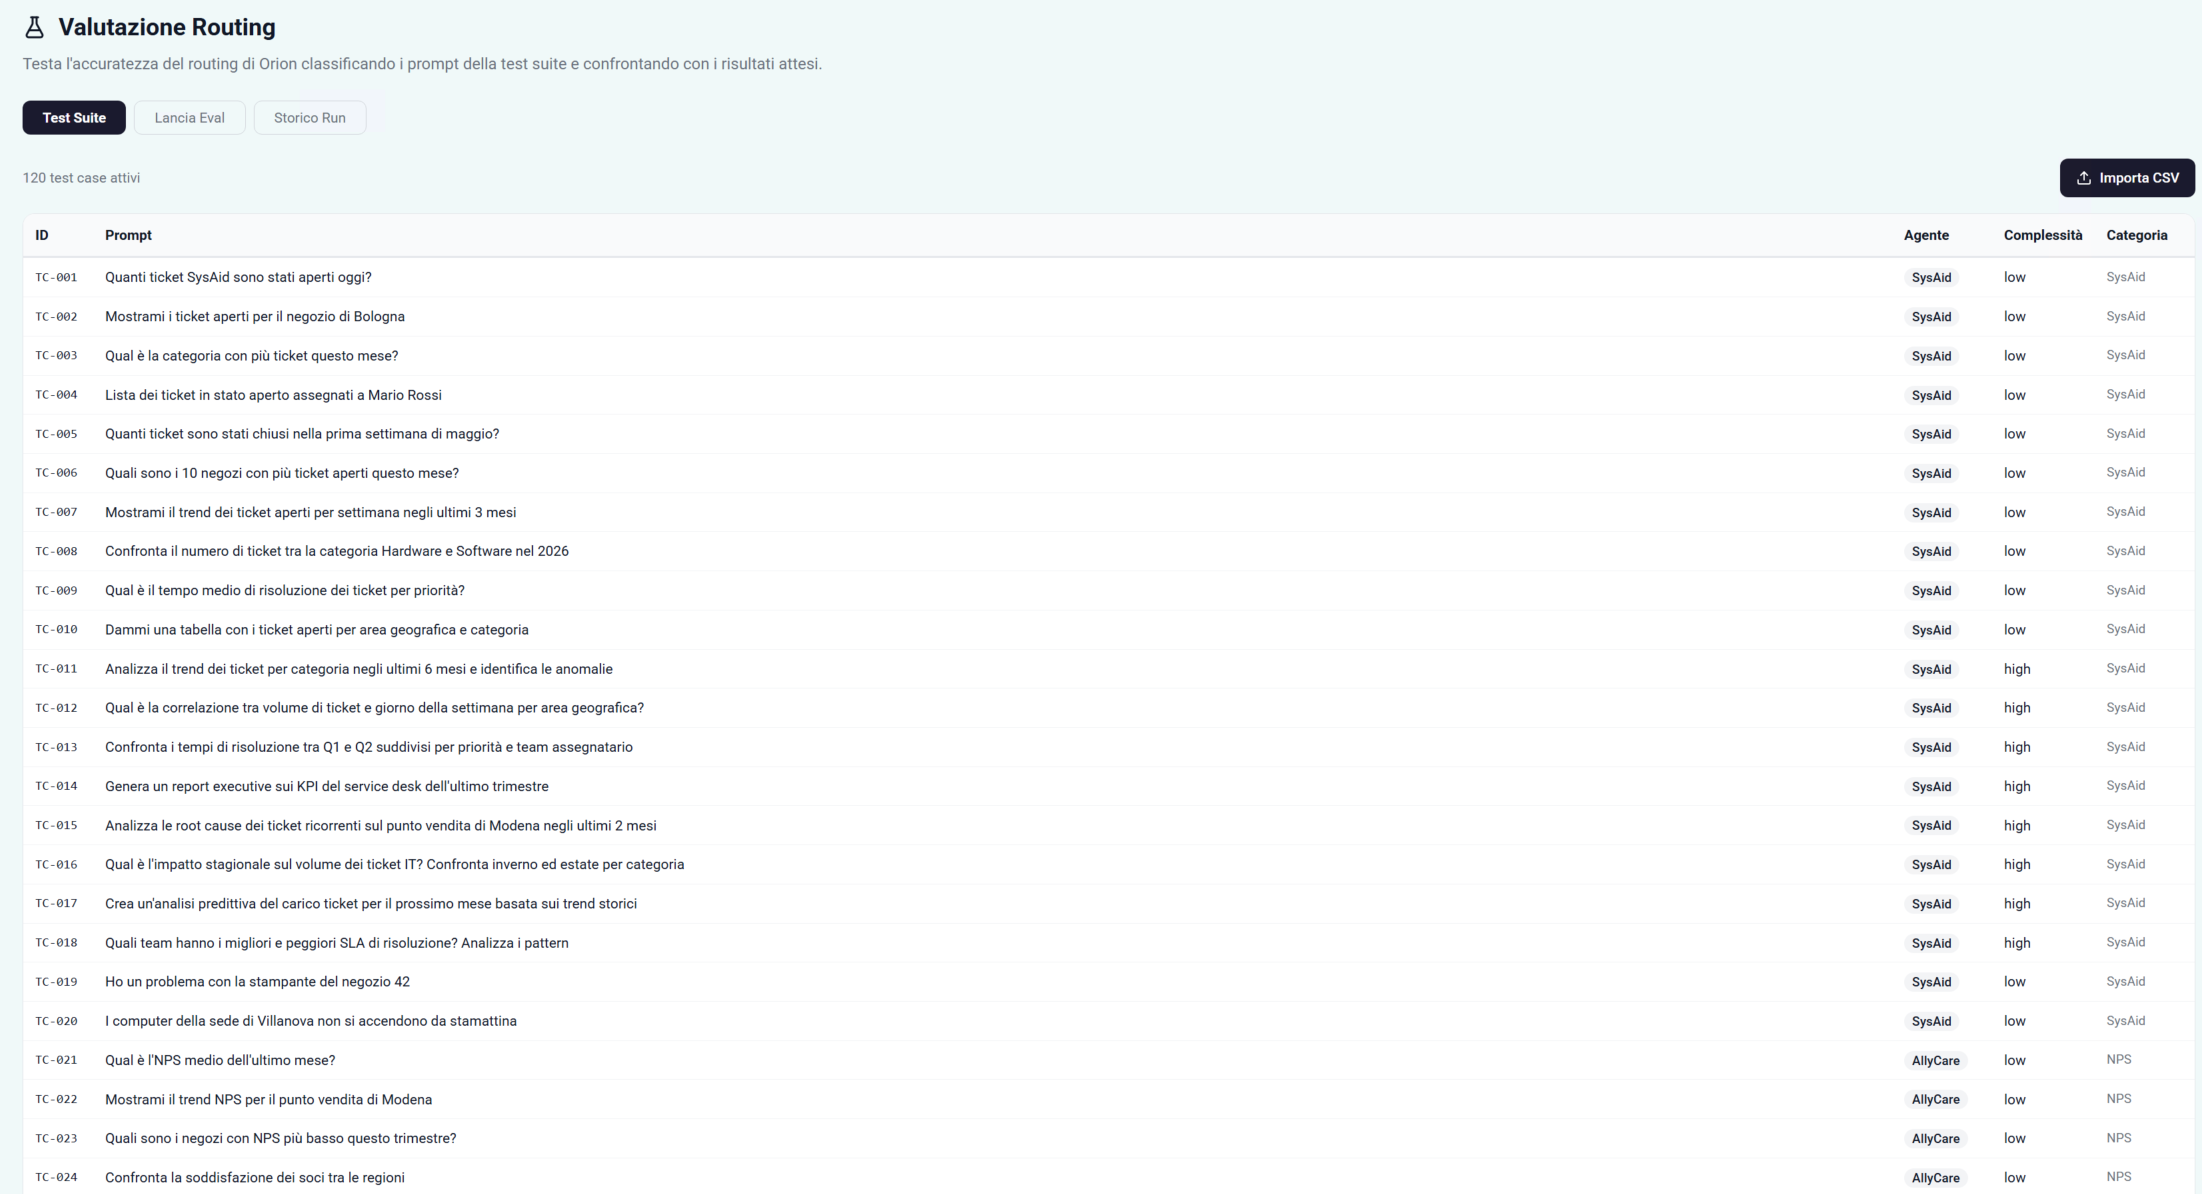
\includegraphics[width=\textwidth]{eval1}
    \caption[Estratto della test suite]{La test suite di valutazione nel tab ``Test Suite'' dell'admin panel di Orion: i 120 prompt etichettati con agente atteso, 
    complessità attesa e categoria tematica, importabili da CSV.}
    \label{fig:test_suite}
\end{figure}

\subsection{Architettura del framework di valutazione}
\label{subsec:eval-admin-page}

La valutazione avviene interamente dalla pagina \emph{Eval Routing} dell'admin panel di Orion (Sez.~\ref{sec:orion-impl-admin}), senza necessità di script CLI esterni o accesso diretto all'infrastruttura di Cooperativa.

\paragraph{Backend (\texttt{eval.py}).} Cinque endpoint REST esposti sotto il prefisso \texttt{/api/\allowbreak orion-admin/\allowbreak eval/}:

\begin{itemize}
  \item \texttt{GET /test-suite}: restituisce i test case attivi dal database.
  \item \texttt{POST /test-suite/import}: importa i test case da un contenuto CSV, sovrascrivendo i precedenti.
  \item \texttt{POST /run}: esegue la valutazione. Per ciascun test case, il backend chiama la funzione \texttt{classify()} \emph{direttamente} (invocazione Python, nessuna chiamata HTTP), 
  confronta l'output con l'atteso, salva il risultato nel database e costruisce il summary.
  \item \texttt{GET /runs}: restituisce la lista delle run passate con metriche aggregate.
  \item \texttt{GET /runs/\{run\_id\}}: restituisce il dettaglio completo di una run specifica.
\end{itemize}

L'invocazione diretta della funzione \texttt{classify()} è molto conveniente: 
il backend admin (\texttt{orion-admin-backend}) include una copia del modulo \texttt{router\_agent.py}, 
rendendo possibile l'import Python diretto senza la necessità di chiamare l'endpoint \texttt{/classify} del backend utente. 

Ogni test case costa una sola chiamata a Gemini Flash ($\sim$0,5~secondi); una run completa di 120~test case richiede circa 60~secondi.

\paragraph{Frontend (\texttt{Eval.tsx}).} Una pagina React organizzata in tre tab (\emph{Test Suite}, \emph{Lancia Eval}, \emph{Storico Run}) 
che integra l'intero ciclo di valutazione in un'unica interfaccia. Il tab \emph{Lancia Eval} visualizza i risultati con KPI card codificate cromaticamente 
(verde se il target è raggiunto, rosso altrimenti), breakdown per agente con barre orizzontali, 
lista dei casi errati espandibile con il reasoning del router, e tabella completa dei risultati con icone di correttezza.

\subsection{Metriche e target}
\label{subsec:eval-metriche}


\begin{table}[htbp]
  \centering
  \caption[Metriche di valutazione e target]{Metriche di valutazione del routing con target dichiarati a priori.}
  \label{tab:eval-metriche}
  \begin{tabular}{llc}
    \toprule
    \textbf{Metrica}                  & \textbf{Definizione}                              & \textbf{Target} \\
    \midrule
    Agent Accuracy                    & $\frac{\text{agente corretto}}{\text{totale}}$     & $\geq 85\%$ \\[3pt]
    Complexity Accuracy               & $\frac{\text{complessità corretta}}{\text{totale}}$ & $\geq 80\%$ \\[3pt]
    Clarification Rate                & $\frac{\text{clarification poste}}{\text{totale}}$  & $< 15\%$ \\[3pt]
    Mean Confidence (correct)         & Media della confidence sui casi corretti            & $\geq 0{,}82$ \\[3pt]
    Mean Confidence (wrong)           & Media della confidence sui casi errati              & $\leq 0{,}65$ \\
    \bottomrule
  \end{tabular}
\end{table}

Le ultime due metriche, prese congiuntamente, valutano la \emph{calibrazione} del confidence score~\cite{kadavath2022knowsknows}: 
un router ben calibrato è sicuro quando ha ragione e dubbioso quando sbaglia. 
Se le due distribuzioni di confidence (corretti vs errati) sono ben separate, la soglia di clarification può essere posizionata in modo efficace.

% =====================================================================
\section{Il prompt del router: anatomia e tecniche}
\label{sec:eval-prompteng}
% =====================================================================

Prima di presentare i risultati è utile esaminare l'oggetto su cui agisce
l'iterazione misurata in questo capitolo: il \emph{system prompt} del router.
Questa sezione ne descrive l'anatomia attraverso estratti della versione
v1.0, riprodotti dal codice pubblicato
(Sez.~\ref{sec:concl-generalizzabilita}, modulo
\texttt{orion-backend/app/agents/router\_agent.py}), e cataloga le tecniche
di prompt engineering che il prompt incorpora, collegandole alla letteratura
introdotta nel background (Sez.~\ref{sec:bg-prompting}); la stessa
catalogazione è poi estesa ai prompt degli agenti verticali, che
costituiscono altrettanti casi applicativi su dati aziendali reali.

\subsection{Anatomia del system prompt}
\label{subsec:eval-prompt-anatomia}

Il prompt è organizzato in blocchi delimitati da intestazioni maiuscole
--- una pratica di \emph{role prompting} con delimitatori espliciti che la
letteratura indica come efficace per ridurre le ambiguità di
parsing~\cite{sahoo2024prompteng_survey}. Il Listato~\ref{lst:prompt-regole}
riporta l'apertura e le regole di classificazione.

\begin{lstlisting}[caption={Estratto del system prompt del router (v1.0): ruolo, blocco agenti e regole di classificazione. Il segno [...] indica omissioni; i segnaposto fra graffe sono compilati a runtime.},label={lst:prompt-regole}]
Sei il modulo di routing di ORION, l'orchestratore AI
dell'organizzazione. Il tuo compito è classificare la richiesta
dell'utente per instradarlo all'agente specializzato più appropriato.

AGENTI DISPONIBILI:
{agents_block}

REGOLE DI CLASSIFICAZIONE:
1. Scegli l'agente il cui dominio corrisponde meglio alla richiesta
   dell'utente.
2. Se la richiesta è ambigua o potrebbe essere gestita da più agenti,
   scegli quello più probabile e indica una confidence più bassa.
3. Se la richiesta è chiaramente fuori dal dominio di tutti gli agenti
   specializzati, usa "self".
4. Saluti, conversazione generica, domande su documenti caricati
   dall'utente, e ricerche web vanno sempre a "self".
5. Per TUTTE le richieste, valuta la complessità in modo binario:
   - "low": domande dirette, conteggi semplici, filtri base, ricerche
     per un singolo criterio, aggregazioni semplici
   - "high": analisi multi-dimensionali, correlazioni, confronti
     temporali articolati, root cause analysis, report executive,
     ragionamento su più metriche incrociate
   La complessità influenza il modello LLM scelto dall'agente
   (es. SysAid usa un modello più potente per richieste complesse).
[...]
\end{lstlisting}

Le regole combinano tre dispositivi distinti. Le regole~1--3 definiscono la
politica di selezione e il comportamento di \emph{default} (la regola~4
assegna esplicitamente a \texttt{self} le classi di richieste più frequenti
e meno informative, sottraendole all'inferenza). La regola~5 definisce le
classi di complessità \emph{per esempi di istanze} anziché per definizione
astratta: è la stessa logica del few-shot
prompting~\cite{brown2020gpt3}, applicata però alla descrizione delle
etichette. La chiusura della regola~5 esplicita al modello la
\emph{conseguenza} della sua decisione (la selezione del modello nel
sub-agente): rendere espliciti gli effetti delle scelte è una pratica
raccomandata per i compiti di classificazione
strumentale~\cite{sahoo2024prompteng_survey}.

Il secondo estratto (Listato~\ref{lst:prompt-confidence}) riguarda la stima
della confidence, il fondamento del meccanismo di clarification
(Sez.~\ref{subsec:orion-confidence}).

\begin{lstlisting}[caption={Estratto del system prompt del router (v1.0): rubrica di confidence e istruzione di deferral.},label={lst:prompt-confidence}]
STIMA DELLA CONFIDENCE:
- 0.90-1.00: la richiesta è chiaramente nel dominio di un singolo
  agente, senza ambiguità
- 0.70-0.89: la richiesta è probabilmente nel dominio indicato, ma ci
  sono elementi di ambiguità
- 0.50-0.69: la richiesta è ambigua, potrebbe appartenere a più domini
- sotto 0.50: la richiesta è troppo vaga per essere classificata con
  sicurezza

Se la confidence è inferiore a {confidence_threshold}, imposta
clarification_needed con una domanda breve e chiara per disambiguare
l'intento dell'utente.
\end{lstlisting}

La confidence non è chiesta come numero libero ma ancorata a una
\emph{rubrica} di quattro fasce con descrizioni operative: è una forma di
\emph{verbalized confidence elicitation}, che la letteratura sulla
calibrazione indica come ragionevolmente affidabile nei modelli di grande
scala~\cite{kadavath2022knowsknows}. L'istruzione finale collega la stima
all'azione: sotto soglia il modello deve formulare esso stesso la domanda di
disambiguazione, realizzando il \emph{deferral} human-in-the-loop ispirato
all'active learning~\cite{settles2012active,diao2023activeprompting}.
Il campo \texttt{reasoning} obbligatorio dell'output (Chain-of-Thought
esplicita~\cite{wei2022cot}) e il vincolo di \emph{guided
generation} sullo schema JSON con \texttt{enum} dinamica
(Sez.~\ref{subsec:orion-output-strutturato},~\cite{willard2023outlines})
completano il quadro: il primo fornisce tracciabilità diagnostica, il
secondo elimina per costruzione i target inesistenti.

Un'ultima proprietà è operativa: il testo del prompt è un \emph{template}
con segnaposto (\texttt{\{agents\_block\}}, \texttt{\{history\_block\}},
\texttt{\{confidence\_threshold\}}, \texttt{\{user\_prompt\}}) compilati a
ogni richiesta, ed è persistito nel database (\texttt{app\_settings}),
modificabile dalla pagina \emph{Router Prompt} dell'admin panel
(Sez.~\ref{sec:orion-impl-admin}) senza rilascio di codice. È questa
proprietà a rendere praticabile il ciclo di iterazione misurato nella
Sez.~\ref{sec:eval-risultati}.

\subsection{Few-shot dinamico: il blocco degli agenti}
\label{subsec:eval-prompt-fewshot}

Il segnaposto \texttt{\{agents\_block\}} è compilato a runtime con la
descrizione dei soli agenti disponibili per l'utente corrente: per ciascuno,
nome, descrizione del dominio ed esempi di richieste tipiche. Il
Listato~\ref{lst:prompt-agente} riporta il blocco di SysAid.

\begin{lstlisting}[caption={Estratto del system prompt del router (v1.0): il blocco descrittivo di SysAid generato a runtime, con gli esempi few-shot.},label={lst:prompt-agente}]
### SysAid (Ticket IT) (key: "sysaid")
Agente specializzato nell'analisi dei ticket IT SysAid. Interroga
BigQuery per cercare, filtrare, aggregare e analizzare i ticket di
assistenza tecnica (service requests). [...] Il modello LLM viene
selezionato automaticamente in base alla complessità della richiesta.
Esempi di richieste tipiche:
  - "Quanti ticket sono stati aperti questa settimana?"
  - "Mostrami i ticket aperti per il negozio di Bologna"
  - "Analizza il trend dei ticket per categoria negli ultimi 6 mesi
     e identifica le anomalie"
  - "Genera un report executive sui KPI del service desk dell'ultimo
     trimestre"
\end{lstlisting}

Gli esempi sono \emph{in-context examples} nel senso di
Brown et al.~\cite{brown2020gpt3}, con due accortezze. La prima è che gli
esempi di ciascun agente sono scelti per coprire entrambe le fasce di
complessità: i primi due del listato modellano richieste \texttt{low}
(conteggio, filtro singolo), gli ultimi due richieste \texttt{high}
(trend con anomalie, report executive); il blocco insegna così
simultaneamente il dominio dell'agente \emph{e} la nozione di complessità
della regola~5. La seconda è che il blocco è \emph{dinamico}: riflette i
soli agenti abilitati per l'utente, in coerenza con l'\texttt{enum}
dell'output strutturato, così che descrizioni e vincoli di schema non
possano mai divergere.

\subsection{Le tecniche nei prompt della suite}
\label{subsec:eval-prompt-tecniche}

Il router non è l'unico componente in cui il comportamento del modello è
governato dal prompt: ciascun agente verticale incorpora tecniche analoghe,
descritte nel Capitolo~\ref{chap:agenti} insieme alla loro funzione. La
Tab.~\ref{tab:eval-tecniche} le riassume in chiave comparata, collegandole
alla letteratura di riferimento.

\begin{table}[htbp]
  \centering
  \caption[Tecniche di prompt engineering nella suite]{Le tecniche di prompt engineering utilizzate nella suite, con riferimento alla letteratura e punto di applicazione.}
  \label{tab:eval-tecniche}
  \small
  \begin{tabular}{p{3.4cm}p{2.6cm}p{7.2cm}}
    \toprule
    \textbf{Tecnica} & \textbf{Riferimento} & \textbf{Applicazione nella suite} \\
    \midrule
    Role prompting e sezioni delimitate & \cite{sahoo2024prompteng_survey}
      & Incipit e struttura a blocchi del router (Listato~\ref{lst:prompt-regole}); prompt di sistema ``collegiali'' degli agenti (Sez.~\ref{sec:agenti-principi}) \\
    In-context examples (few-shot) & \cite{brown2020gpt3}
      & Esempi di richieste tipiche per agente nel blocco agenti del router (Listato~\ref{lst:prompt-agente}) \\
    Chain-of-Thought esplicita & \cite{wei2022cot}
      & Campo \texttt{reasoning} obbligatorio del router; disciplina \texttt{\#\#\# RAGIONAMENTO}/\texttt{\#\#\# RISPOSTA} degli agenti (Sez.~\ref{subsec:agenti-auth}) \\
    Guided generation (output strutturato) & \cite{willard2023outlines}
      & \texttt{response\_schema} JSON con \texttt{enum} dinamica nel router (Sez.~\ref{subsec:orion-output-strutturato}); classificatore di corpus di CooPolicy (Sez.~\ref{subsec:coopolicy-multicorpus}) \\
    Confidence verbalizzata con rubrica & \cite{kadavath2022knowsknows}
      & Le quattro fasce della stima di confidence (Listato~\ref{lst:prompt-confidence}) \\
    Deferral / clarification & \cite{settles2012active,diao2023activeprompting}
      & \texttt{clarification\_needed} sotto soglia di confidence (Sez.~\ref{subsec:orion-confidence}) \\
    Schema injection selettiva e glossario semantico & \cite{pourreza2023dinsql}
      & AllyCare e SysAid: schema delle sole tabelle rilevanti, glossario delle colonne in italiano, anagrafica negozi iniettata (Sez.~\ref{subsec:allycare-schema}) \\
    Regole negative e di dominio & \cite{sahoo2024prompteng_survey}
      & Filtri di validità SQL e \texttt{UPPER(TRIM(...))} (Sez.~\ref{subsec:allycare-schema}); ``gerarchia della verità'' e fiducia nel tool (Sez.~\ref{subsec:allycare-discipline}); le otto regole non negoziabili di CooPolicy (Sez.~\ref{subsec:coopolicy-generation}) \\
    Self-correction & \cite{pourreza2023dinsql}
      & Errori SQL reimmessi come \texttt{function\_response} nel ciclo agentico (Sez.~\ref{subsec:allycare-tools}) \\
    \bottomrule
  \end{tabular}
\end{table}

Per diverse di queste tecniche l'effetto è riscontrabile negli esiti
documentati nel resto della tesi. La ``fiducia nel tool'' di AllyCare ha
eliminato in fase di test la classe di errori in cui il modello, ricalcolando
mentalmente, contraddiceva il risultato della propria query
(Sez.~\ref{subsec:allycare-discipline}). Le regole SQL di dominio si
riflettono nell'alta quota di SQL eseguibile prodotto dagli agenti
Text-to-SQL ($23/25$ e $25/25$ nelle run della Sez.~\ref{subsec:eval-text2sql}).
La guided generation con \texttt{enum} elimina per costruzione gli
instradamenti verso agenti inesistenti, riducendo il fallback difensivo a
salvaguardia residuale (Sez.~\ref{subsec:orion-impl-router}). La rubrica di
confidence, infine, è il presupposto della calibrazione verificata in
Sez.~\ref{subsec:eval-confidence-cal}.

Il prompt v1.0 qui descritto non è un primo tentativo: è l'esito delle
iterazioni informali condotte durante lo sviluppo della suite, guidate
dall'osservazione qualitativa dei log di routing.
% TODO F3.5: arricchire con 2-3 passate di tuning pre-v1.0 documentate
% (recuperare versioni storiche del prompt da app_settings / history
% Bitbucket e note di sviluppo).
L'iterazione successiva (v1.0~$\rightarrow$~v1.1), condotta invece con il
metodo quantitativo di questo capitolo, è documentata nella
Sez.~\ref{subsec:eval-iterazione}.

% =====================================================================
\section{Risultati}
\label{sec:eval-risultati}
% =====================================================================

\subsection{Run v1.0: primo prompt}
\label{subsec:eval-v10}

La prima run di valutazione (prompt version v1.0) ha prodotto i seguenti risultati su 120~test case (Tab.~\ref{tab:eval-v10}):

\begin{table}[htbp]
  \centering
  \caption[Risultati della run v1.0]{Risultati della run v1.0 (120 test case, primo system prompt).}
  \label{tab:eval-v10}
  \begin{tabular}{lcc}
    \toprule
    \textbf{Metrica}             & \textbf{Valore}  & \textbf{Target} \\
    \midrule
    Agent Accuracy               & $99{,}2\%$ (119/120) & $\geq 85\%$ \\
    Complexity Accuracy          & $88{,}3\%$ (106/120) & $\geq 80\%$ \\
    \bottomrule
  \end{tabular}
\end{table}

L'accuracy globale supera il target del $85\%$ fin dalla prima iterazione. Di seguito il breakdown per agente (Tab.~\ref{tab:eval-v10-breakdown}):

\begin{table}[htbp]
  \centering
  \caption[Breakdown per agente --- v1.0]{Agent accuracy per agente target nella run v1.0.}
  \label{tab:eval-v10-breakdown}
  \begin{tabular}{lcl}
    \toprule
    \textbf{Agente}   & \textbf{Accuracy}     & \textbf{Note} \\
    \midrule
    SysAid            & 100\% (36/36)         & Perfetto \\
    CooPolicy         & 100\% (33/33)         & Perfetto \\
    AllyCare          & 95\% (20/21)          & Eccellente \\
    Self (Orion)      & 100\% (30/30)         & Perfetto \\
    \bottomrule
  \end{tabular}
\end{table}

\begin{figure}[htbp]
    \centering
    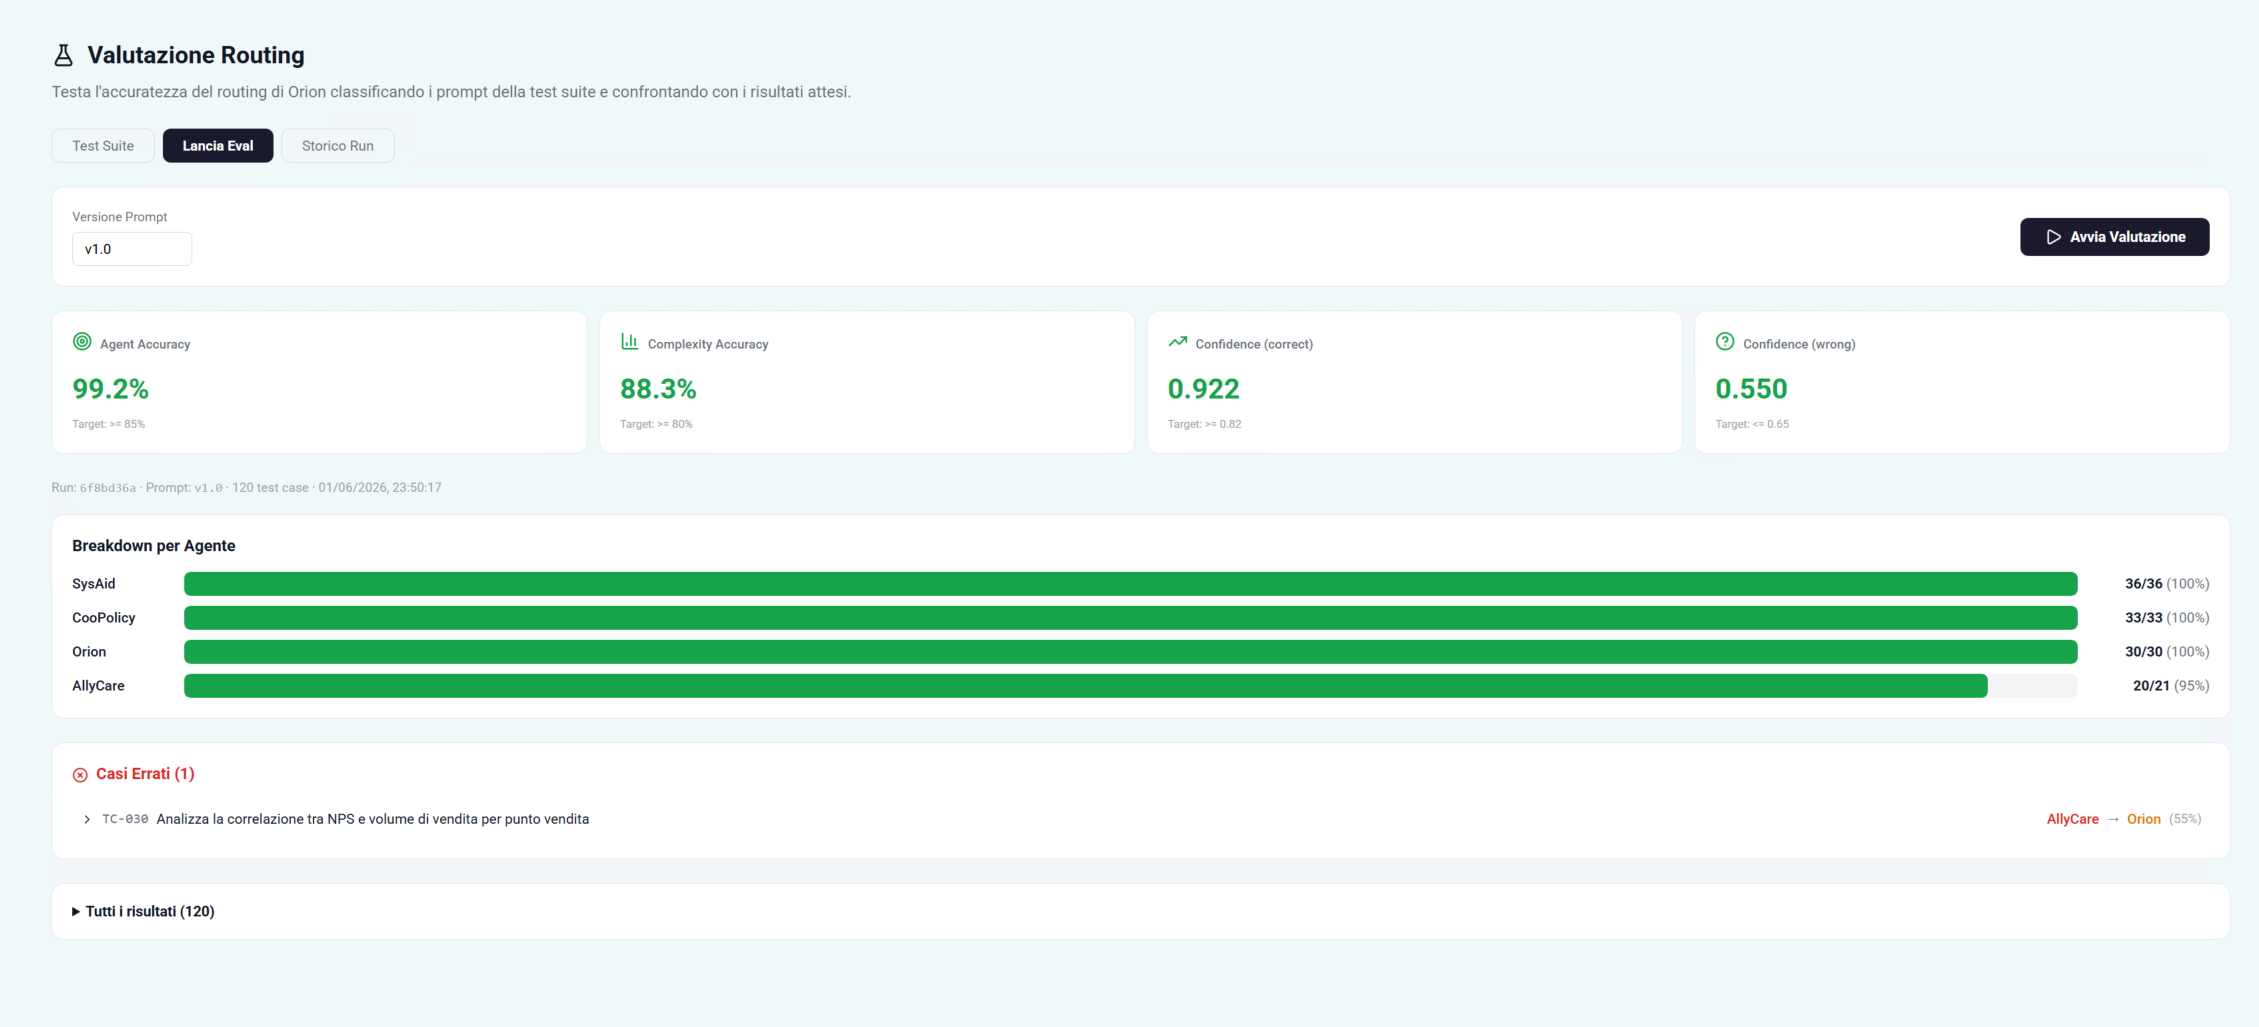
\includegraphics[width=\textwidth]{eval2}
    \caption[Risultati della run v1.0 nell'admin panel]{La pagina di valutazione al termine della run v1.0: le quattro KPI card 
    (agent accuracy, complexity accuracy, confidence media sui casi corretti e sugli errati) e il breakdown per agente.}
    \label{fig:accuracy_per_agent}
\end{figure}

\subsection{Analisi degli errori della v1.0}
\label{subsec:eval-errori-v10}

L'errore di classificazione della v1 ricade in questo pattern: 

\paragraph{Pattern 1: Correlazione cross-dataset non riconosciuta (1~errore).} Il prompt ``Analizza la correlazione tra NPS e volume di vendita per punto vendita'' 
viene instradato a \texttt{self} anziché ad \texttt{allycare}, perché il router non riconosce che i dati NPS sono necessari per l'analisi. 
È l'unico errore, con confidence bassa (0,55), segnale che il router stesso percepiva l'incertezza.

\subsection{Iterazione del prompt: v1.1}
\label{subsec:eval-iterazione}

Sulla base dell'analisi sono state apportate queste modifiche, per cercare di eliminare l'errore e migliorare la complexity accuracy:

\begin{enumerate}
  \item \textbf{Regola 8: Correlazioni cross-dataset.} Aggiunta la regola che richieste che \emph{richiedono dati} di un agente specializzato (anche se formulate in modo generico) 
  vanno instradate a quell'agente.

  \item \textbf{Complessità.} È stata modificata la classificazione per cercare di fare correttamente catalogare come ``low'' le ricerche a singola query o i confronti semplici.

\end{enumerate}

Entrambe le modifiche sono istanze delle tecniche catalogate nella
Sez.~\ref{sec:eval-prompteng}: la Regola~8 è una \emph{regola di precedenza}
esplicita, che risolve i conflitti fra domini sovrapposti a favore
dell'agente che detiene i dati necessari; la revisione dei criteri di
complessità arricchisce la definizione per istanze delle classi
\texttt{low}/\texttt{high} (Listato~\ref{lst:prompt-regole}, regola~5) con i
casi di confine emersi dall'analisi degli errori.
% TODO F3.5: inserire qui il diff testuale effettivo v1.0 -> v1.1 del prompt
% (recuperare la v1.1 dalla tabella app_settings via pagina Router Prompt).

La run v1.1 è stata eseguita sullo \emph{stesso} gold standard della v1.0 modificando esclusivamente il system prompt del router. La Tab.~\ref{tab:eval-v11} confronta le due run.

\begin{table}[htbp]
  \centering
  \caption[Confronto fra le run v1.0 e v1.1]{Confronto fra le run v1.0 e v1.1 sul medesimo gold standard di 120 test case. Cambia esclusivamente il system prompt del router.}
  \label{tab:eval-v11}
  \begin{tabular}{lcc}
    \toprule
    \textbf{Metrica}                 & \textbf{v1.0} & \textbf{v1.1} \\
    \midrule
    Agent Accuracy                   & $99{,}2\%$      & $99{,}2\%$ \\
    Complexity Accuracy              & $88{,}3\%$      & $93{,}3\%$ \\
    Errori (su 120)                  & 1               & 1 \\
    Confidence media (corretti)      & $0{,}922$       & $0{,}922$ \\
    Confidence media (errati)        & $0{,}55$        & $0{,}5$ \\
    \bottomrule
  \end{tabular}
\end{table}

Il guadagno più netto è sulla \emph{complexity accuracy} ($+5{,}0$~punti percentuali): le regole aggiunte hanno reso più stabile la distinzione low/high. 
L'\emph{agent accuracy} invece non migliora: la Regola~8 non è bastata a correggere la correlazione cross-dataset dell'errore, che ricompare a bassa confidence. 


\begin{figure}[htbp]
  \centering
  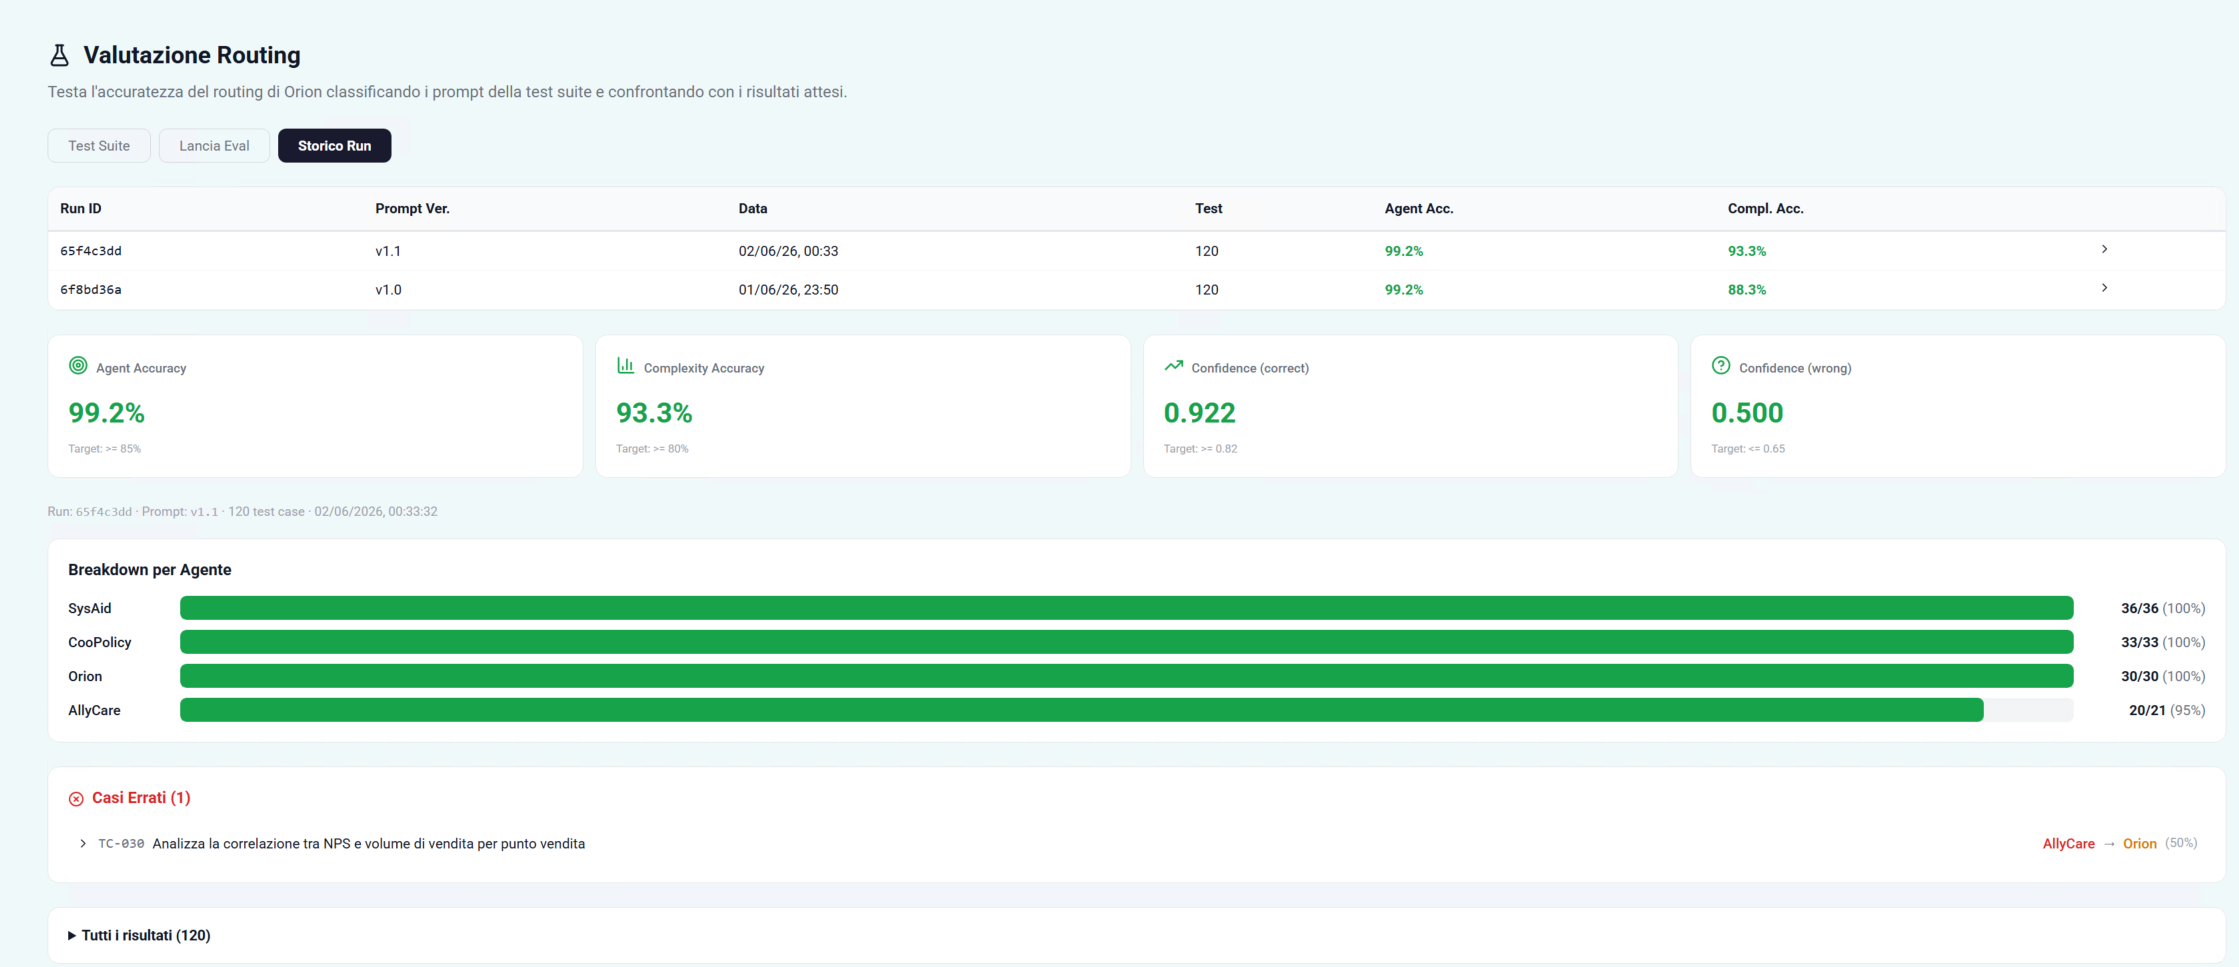
\includegraphics[width=\textwidth,keepaspectratio]{eval4}
  \caption[Risultati della run v1.1 nell'admin panel]{Risultati della run v1.1 nell'admin panel, con lo storico delle due run sul medesimo gold standard. 
  Le KPI card e il breakdown per agente si riferiscono alla v1.1.}
  \label{fig:eval_v11}
\end{figure}

\subsection{Calibrazione del confidence score}
\label{subsec:eval-confidence-cal}

La calibrazione del confidence score è verificata confrontando la distribuzione della confidence sui casi corretti e quella sui casi errati. 
Un router ben calibrato presenta due distribuzioni ben separate: confidence alta sui casi corretti, confidence bassa sui casi errati.

Nella run v1.0 la confidence media è risultata pari a $0{,}922$ sui casi corretti e $0{,}55$ sul caso errato;
la seconda run l'ha ulteriormente abbassata a $0{,}5$.

% =====================================================================
\section{Valutazione della qualità degli agenti verticali}
\label{sec:eval-agenti}
% =====================================================================

La valutazione del routing (Sez.~\ref{sec:eval-risultati}) misura se Orion sceglie l'agente \emph{giusto}, ma non se l'agente scelto risponde \emph{bene}. 
Questa sezione colma quel divario valutando direttamente la qualità dei sub-agenti, con due metodologie distinte a seconda della forma di grounding: 
\emph{execution accuracy} per gli agenti Text-to-SQL (SysAid, AllyCare) e \emph{faithfulness} con \emph{answer relevancy} per l'agente RAG (CooPolicy). 
Entrambe sono applicazioni dirette delle metriche introdotte nel Capitolo~\ref{chap:background} (Sez.~\ref{subsec:bg-text2sql} e~\ref{sec:bg-ragas}).

Il codice della valutazione è pubblicato nel modulo \texttt{evaluation/} del repository (Sez.~\ref{sec:concl-generalizzabilita}): 
gli script invocano gli \emph{endpoint reali} degli agenti così che la misura sia end-to-end e non su una riproduzione parziale del sistema.

\subsection{Text-to-SQL: execution accuracy}
\label{subsec:eval-text2sql}

La metrica adottata è l'\emph{execution accuracy} (o \emph{denotation accuracy}), lo standard dei benchmark Spider~\cite{yu2018spider} e 
BIRD~\cite{li2023bird}: una query generata è corretta se, eseguita, produce lo \emph{stesso result-set} della query di riferimento (\emph{gold}), 
indipendentemente dalla sua formulazione testuale. Rispetto al confronto sintattico fra stringhe SQL, l'execution accuracy è la misura corretta perché query 
diverse possono essere semanticamente equivalenti.

\paragraph{Protocollo.} Per ciascuna domanda di un gold standard etichettato (domanda in linguaggio naturale + query SQL di riferimento) lo script invoca l'agente sul suo 
endpoint di produzione, estrae le query SQL effettivamente eseguite (esposte dall'agente nel campo \texttt{queries}),
le esegue su BigQuery insieme alla gold e ne confronta i result-set in modo order-insensitive e robusto a casing e arrotondamenti. 
Si riportano due metriche: \textbf{EX (final)}, che richiede il match con l'ultima query del turno (quella che produce la risposta finale), ed \textbf{EX (any)}, 
che ammette il match con almeno una delle query eseguite; la distanza fra le due separa gli errori di generazione SQL dagli errori di selezione della query conclusiva.

\begin{table}[htbp]
  \centering
  \caption[Execution accuracy degli agenti Text-to-SQL]{Execution accuracy degli agenti Text-to-SQL su un gold standard di domande etichettate con SQL di riferimento. La complessità segue la stessa distinzione low/high del routing.}
  \label{tab:eval-text2sql}
  \begin{tabular}{lcccc}
    \toprule
    \textbf{Agente} & \textbf{N} & \textbf{EX (final)} & \textbf{EX (any)} & \textbf{IC 95\% (Wilson)} \\
    \midrule
    AllyCare (NPS)      & 25 & 80{,}0\% & 80{,}0\% & $[60{,}9\% ,\, 91{,}1\%]$ \\
    SysAid (ticketing)  & 25 & 84{,}0\% & 84{,}0\% & $[65{,}3\% ,\, 93{,}6\%]$ \\
    \bottomrule
  \end{tabular}
\end{table}

AllyCare raggiunge un'execution accuracy dell'$80\%$ (20/25) e SysAid dell'$84\%$ (21/25), con SQL eseguibile prodotto rispettivamente in $23/25$ e $25/25$ dei casi. 
La coincidenza fra EX (final) ed EX (any) indica che, quando l'agente sbaglia, sbaglia la query stessa e non la mera selezione di quella conclusiva. 
Gli errori si concentrano su due classi note nella letteratura Text-to-SQL: (i)~le \emph{aggregazioni con regole di dominio implicite} come 
il calcolo dell'NPS (formula promotori/detrattori), le medie con filtri di validità (\texttt{voto\_item >= 0}) e le percentuali per AllyCare; 
le aggregazioni temporali per SysAid, dove l'interpretazione dell'agente diverge da quella codificata nella query gold; 
(ii)~alcuni casi in cui l'agente risponde in modo discorsivo senza eseguire SQL. Si osserva inoltre un effetto del \emph{non-determinismo}: 
un conteggio elementare classificato correttamente in un'esecuzione può fallire in un'altra, segnale che parte della varianza è stocastica e non sistematica 
(cfr. Sez.~\ref{subsec:eval-limiti}). Va infine ricordato che una quota di questi disaccordi è imputabile all'etichettatura del gold standard (un solo annotatore): 
su domande con regole di business sfumate la query di riferimento è una scelta progettuale. Gli intervalli di confidenza al $95\%$ (metodo di Wilson) sono ampi, $[60{,}9\%,\,91{,}1\%]$ per AllyCare
e $[65{,}3\%,\,93{,}6\%]$ per SysAid, conseguenza diretta del campione ridotto ($n=25$): i valori vanno letti come stime puntuali con incertezza non trascurabile.
Il breakdown di queste metriche per fascia di complessità, rilevante per il trade-off costo--qualità, è analizzato nella Sez.~\ref{subsec:eval-cq-breakdown}.

\subsection{RAG: faithfulness e answer relevancy}
\label{subsec:eval-rag}

Per CooPolicy si adottano due metriche del framework RAGAS~\cite{es2023ragas}, calcolate con il paradigma \emph{LLM-as-judge}~\cite{zheng2023llmjudge}: 
la \textbf{faithfulness} (frazione delle affermazioni della risposta supportate dai frammenti recuperati, misura anti-allucinazione) e l'\textbf{answer relevancy} 
(pertinenza della risposta alla domanda). Il gold standard distingue domande \emph{nel} corpus, su cui si misurano le due metriche e l'\emph{answer rate}, 
da domande \emph{fuori} corpus, su cui si misura il \emph{tasso di corretto rifiuto}: per un agente vincolato al solo materiale recuperato (Sez.~\ref{subsec:coopolicy-generation}), 
rifiutare correttamente una domanda fuori dominio è esso stesso un comportamento desiderato.

\begin{table}[htbp]
  \centering
  \caption[Metriche RAG di CooPolicy]{Metriche di qualità del RAG di CooPolicy, calcolate con LLM-as-judge (Gemini~2.5 Pro) su un gold standard di domande in-corpus e fuori-corpus.}
  \label{tab:eval-rag}
  \begin{tabular}{lc}
    \toprule
    \textbf{Metrica} & \textbf{Valore} \\
    \midrule
    Faithfulness media (in-corpus)              & 0{,}73 \\
    Answer relevancy media (in-corpus)          & 0{,}85 \\
    Answer rate (in-corpus)                     & 100\% (20/20) \\
    Corretto rifiuto (fuori-corpus)             & 80\% (4/5) \\
    Citazioni sulle risposte in-corpus          & 100\% (20/20) \\
    \bottomrule
  \end{tabular}
\end{table}

CooPolicy risponde a tutte le domande in corpus ($20/20$), sempre corredando la risposta di citazioni alle fonti, 
e rifiuta correttamente $4$ delle $5$ domande fuori corpus: l'unico scivolone è una richiesta di traduzione, 
a cui l'agente risponde dalla conoscenza parametrica anziché astenersi, comportamento innocuo ma formalmente fuori mandato. 
La faithfulness media ($0{,}73$) e l'answer relevancy ($0{,}85$) indicano risposte pertinenti e in larga parte ancorate al materiale recuperato, 
ma con \emph{varianza elevata}: diverse risposte sono pienamente fedeli (faithfulness $\geq 0{,}95$), 
altre contengono affermazioni non supportate dagli \emph{snippet} recuperati ($< 0{,}4$). 
Il valore va letto come stima \emph{conservativa}: il giudizio di grounding è calcolato sugli \emph{snippet} di 300~caratteri esposti dall'agente, 
non sul documento integrale, e penalizza quindi affermazioni corrette ma supportate da porzioni di documento non incluse nello snippet.

\paragraph{Limiti.} Le due valutazioni ereditano i limiti generali dell'impianto sperimentale (Sez.~\ref{subsec:eval-limiti}: dimensione del gold standard, bias del costruttore) e ne aggiungono di specifici.
L'execution accuracy dipende dalla correttezza delle query gold, etichettate da un singolo annotatore; il giudizio di faithfulness è affidato a un LLM, 
con i noti bias di posizione, lunghezza e auto-preferenza~\cite{zheng2023llmjudge}, e valuta il \emph{grounding} sugli snippet recuperati (300~caratteri) 
anziché sul documento integrale. Restano dunque misure indicative, utili a stabilire un \emph{ordine di grandezza} della qualità degli agenti e una base di partenza riproducibile, 
non un giudizio definitivo.

% =====================================================================
\section{Ottimizzazione costo--qualità}
\label{sec:eval-costo-qualita}
% =====================================================================

Il routing per complessità è il dispositivo con cui la suite realizza il
trade-off costo--qualità introdotto nel background
(Sez.~\ref{sec:bg-routing}), e opera su due livelli: all'interno degli
agenti, dove l'etichetta \texttt{low}/\texttt{high} seleziona il modello
(Gemini Flash o Pro per Vera, CooPolicy e AllyCare; Gemini Flash o Claude
Sonnet per SysAid, Sez.~\ref{subsec:vera-routing}); e nell'orchestratore,
dove il router stima la complessità e la propaga ai sub-agenti
(Sez.~\ref{subsec:orion-output-strutturato}). Rispetto ai sistemi di
riferimento, il meccanismo è una stima \emph{ex ante} a passaggio singolo:
non un cascade a tentativi successivi come
FrugalGPT~\cite{chen2023frugalgpt}, né un classificatore appreso su dati di
preferenza come RouteLLM~\cite{ong2024routellm}. Questa sezione ne esamina
i due lati: la struttura del risparmio (RQ6, lato costo) e il breakdown
della qualità per fascia di complessità (RQ6, lato qualità).

\subsection{Distribuzione della complessità e struttura del costo}
\label{subsec:eval-cq-costo}

Sul gold standard di 120 casi --- costruito per riflettere la composizione
del traffico atteso (Sez.~\ref{subsec:eval-gold-standard}) --- l'etichetta
di complessità è \texttt{low} in 104 casi ($86{,}7\%$) e \texttt{high} nei
restanti 16 ($13{,}3\%$). Indicando con $f_{\mathrm{low}}$ e
$f_{\mathrm{high}}$ le due frazioni e con $c_{\mathrm{low}}$ e
$c_{\mathrm{high}}$ i costi medi di una richiesta servita rispettivamente
dal modello economico e dal modello premium, il costo medio per richiesta
con routing è
\[
  c_{\mathrm{routing}} = f_{\mathrm{low}} \, c_{\mathrm{low}} + f_{\mathrm{high}} \, c_{\mathrm{high}},
\]
e il risparmio rispetto al servire ogni richiesta con il modello premium
vale
\[
  S \;=\; \frac{c_{\mathrm{high}}}{c_{\mathrm{routing}}}
    \;=\; \frac{\rho}{f_{\mathrm{low}} + f_{\mathrm{high}}\,\rho},
  \qquad \rho = \frac{c_{\mathrm{high}}}{c_{\mathrm{low}}},
\]
dove $\rho$ è il rapporto di costo fra i due modelli. Con la distribuzione
osservata, $S$ cresce con $\rho$ fino al limite asintotico
$1/f_{\mathrm{high}} = 7{,}5$: a titolo illustrativo, per $\rho = 5$ il
routing riduce il costo dell'inferenza di un fattore $3{,}3$, per
$\rho = 10$ di un fattore $4{,}5$, per $\rho = 20$ di un fattore $5{,}7$.
Il valore effettivo di $\rho$ dipende dai listini per token dei modelli e
dal volume medio di token per richiesta, misurabile dalla tabella
\texttt{chat\_logs} che registra i token in/out di ogni interazione
(Sez.~\ref{subsec:agenti-security}); la conversione del modello in valori
monetari è discussa fra i limiti (Sez.~\ref{subsec:eval-limiti}).
% TODO F3.3: token medi in/out per richiesta, per agente e modello
% (query su chat_logs in ambiente GCP).
% TODO F3.6: listini per Mtoken verificati (giugno 2026) di Gemini 2.5
% Flash/Pro su Vertex AI e Claude Sonnet 4.6 — calcolare rho effettivo e
% istanziare S. NON inserire numeri non verificati.
Al costo della risposta si somma quello del routing step di Orion, una
chiamata Flash per ogni richiesta, trascurabile per costruzione rispetto
alla generazione della risposta completa
(Sez.~\ref{subsec:orion-model-routing}).

% TODO F3.1: subsection "Il costo del router: Flash vs Pro" — run della
% test suite v1.1 con router su Gemini 2.5 Pro (etichetta "v1.1-pro")
% dall'admin panel: confrontare agent/complexity accuracy e costo per
% chiamata, a supporto sperimentale della scelta motivata in
% Sez. subsec:orion-model-routing e Tab. tab:orion-decisioni.

\subsection{Qualità per fascia di complessità}
\label{subsec:eval-cq-breakdown}

Il presupposto del routing è che il risparmio non degradi la qualità: le
richieste semplici devono essere servite adeguatamente dal modello
economico e quelle complesse dal modello premium. Una verifica si ottiene
disaggregando l'execution accuracy degli agenti Text-to-SQL
(Sez.~\ref{subsec:eval-text2sql}) per fascia di complessità del gold
standard --- la stessa etichetta che, attraverso la stima del
classificatore, determina il modello utilizzato. La
Tab.~\ref{tab:eval-cq-breakdown} riporta il breakdown, calcolato sulle
medesime run della Sez.~\ref{subsec:eval-text2sql}.

\begin{table}[htbp]
  \centering
  \caption[Execution accuracy per fascia di complessità]{Breakdown dell'execution accuracy per fascia di complessità del gold standard, con il modello che serve ciascuna fascia. Stesse run della Tab.~\ref{tab:eval-text2sql}.}
  \label{tab:eval-cq-breakdown}
  \small
  \begin{tabular}{llccc}
    \toprule
    \textbf{Agente} & \textbf{Fascia (modello)} & \textbf{N} & \textbf{EX (final)} & \textbf{IC 95\% (Wilson)} \\
    \midrule
    AllyCare & low (Gemini 2.5 Flash) & 17 & $82{,}4\%$ (14/17) & $[59{,}0\%,\,93{,}8\%]$ \\
    AllyCare & high (Gemini 2.5 Pro)  & 8  & $75{,}0\%$ (6/8)   & $[40{,}9\%,\,92{,}9\%]$ \\
    SysAid   & low (Gemini 2.5 Flash) & 16 & $75{,}0\%$ (12/16) & $[50{,}5\%,\,89{,}8\%]$ \\
    SysAid   & high (Claude Sonnet 4.6) & 9 & $100\%$ (9/9)     & $[70{,}1\%,\,100\%]$ \\
    \bottomrule
  \end{tabular}
\end{table}

Due osservazioni. La prima: sulle richieste complesse la qualità non
degrada --- l'esito peggiore per un sistema con routing sarebbe
un'accuratezza bassa proprio sulla fascia \texttt{high}, e il campione
mostra l'opposto, con il code path Claude Sonnet di SysAid che non commette
errori ($9/9$). La seconda: gli errori si concentrano sulla fascia
\texttt{low} servita dal modello economico ($12/16$ per SysAid), dove si
era già osservata una componente di varianza stocastica
(Sez.~\ref{subsec:eval-text2sql}): alcune richieste semplici falliscono per
instabilità più che per incapacità sistematica. Il margine di miglioramento
più ampio, dunque, non sta nell'estendere l'uso del modello premium ma nello
stabilizzare il comportamento del modello economico sulle richieste di
routine, oppure nel rivedere il confine fra le due classi di complessità.

\paragraph{Limiti del breakdown.} Tre cautele nella lettura.
(i)~I campioni per fascia sono piccoli (8--17 casi) e gli intervalli di
Wilson conseguentemente ampi. (ii)~Le due fasce contengono domande diverse
per costruzione: il confronto non misura la differenza fra modelli a parità
di domanda (servirebbe un disegno controllato con le stesse domande su
entrambi i code path); misura però la qualità del sistema così come operato
dal routing, che è la grandezza rilevante per l'utente finale.
(iii)~L'attribuzione del code path avviene tramite l'etichetta del gold
standard: in modalità standalone l'agente stima localmente la complessità
(Sez.~\ref{subsec:allycare-tools}) e su una minoranza di casi la stima può
divergere dall'etichetta; il breakdown va quindi letto come un \emph{proxy}
del code path effettivamente percorso.

La prospettiva di questa sezione è il costo marginale per richiesta; la
sezione successiva completa il quadro economico spostandosi sul costo di
adozione della piattaforma.

% =====================================================================
\section{Valutazione economica}
\label{sec:eval-costi}
% =====================================================================

La motivazione di costo (Cap.~\ref{chap:introduzione}) merita una verifica quantitativa, sia pure indicativa:
si costruisce un modello \emph{parametrico} con assunzioni esplicite e facilmente aggiornabili;
il calcolatore è incluso nel modulo \texttt{evaluation/cost\_model.py}.
L'obiettivo non è una stima contabile precisa, ma il confronto fra due modelli di costo: quello di licenze SaaS nominali per l'intera popolazione
e quello di una piattaforma a consumo come quella realizzata.

\paragraph{Assunzioni.} Si considera la popolazione di dipendenti \emph{potenzialmente abilitabili} a una licenza: in Coop Alleanza si tratta di circa $N \approx 4\,000$ figure con mansioni d'ufficio. 
Le suite SaaS di AI generativa per l'enterprise
(assistenti integrati nella suite di produttività o chatbot dedicati) hanno, a listino pubblico nel 2026, un prezzo dell'ordine di \texteuro20--30 per utente al mese
\footnote{Il riferimento è ai prezzi di listino pubblici dei principali assistenti enterprise (es. \texteuro30/utente/mese per le suite di produttività integrate), 
convertiti per omogeneità con il resto della tesi. Il valore è un parametro del modello, non un dato dell'organizzazione.}; nel modello si adotta il valore mediano di \texteuro25.
La piattaforma realizzata, al contrario, ha un costo dominato dal consumo: chiamate ai modelli su Vertex AI,
esecuzione serverless su Cloud Run (che scala a zero) e servizi managed di base. 
La differenza strutturale è che il SaaS è tariffato \emph{per utente abilitato}, la piattaforma \emph{per utilizzo effettivo}, ed è proprio su questo divario
che si fonda il vantaggio economico.

Il punto cruciale è che \emph{avere accesso} a uno strumento di AI non equivale a \emph{usarlo}. I dati di adozione lo confermano: secondo Gallup~\cite{gallup2026aiwork},
fra i lavoratori in ruoli d'ufficio (\emph{remote-capable}) solo il $40\%$ usa l'AI almeno qualche volta a settimana e il $19\%$ ogni giorno;
The Conference Board~\cite{conferenceboard2023genai} stima un uso frequente o regolare attorno al $31\%$. Si assume quindi che la frazione di utenti realmente attivi sia compresa
fra il $19\%$ (uso quotidiano) e il $40\%$ (uso frequente) della popolazione abilitabile, con un volume dell'ordine di $30$--$60$ richieste mensili per utente attivo.
Il modello è \emph{robusto} rispetto alle due letture: come mostra la Tab.~\ref{tab:eval-costi}, entrambe convergono su $\sim0{,}55$~milioni di richieste l'anno
e un costo di piattaforma di $\sim$\texteuro$30$~mila.

\begin{table}[htbp]
  \centering
  \caption[Confronto economico a ordini di grandezza]{Confronto annuo fra licenze SaaS nominali e piattaforma a consumo, 
  per la popolazione di $N\approx4\,000$ dipendenti abilitabili di Coop Alleanza. I valori sono parametrici (vedi \texttt{cost\_model.py}) 
  e la frazione di utenti attivi è ancorata ai dati di adozione di Gallup~\cite{gallup2026aiwork}.}
  \label{tab:eval-costi}
  \small
  \setlength{\tabcolsep}{3pt}
  \begin{tabular}{lcr}
    \toprule
    \textbf{Voce} & \textbf{Parametro} & \textbf{Costo annuo (ordine)} \\
    \midrule
    \multicolumn{3}{l}{\emph{Scenario A --- licenze SaaS nominali}} \\
    Licenze per intera popolazione & $N=4\,000 \times {}$\texteuro$25$/mese & $\sim{}$\texteuro$1{,}2\,$M \\
    \midrule
    \multicolumn{3}{l}{\emph{Scenario B --- piattaforma a consumo (realizzata)}} \\
    Utenti realmente attivi & $19$--$40\%$ di $N$ (Gallup) & --- \\
    Richieste/utente attivo/mese & $\sim30$--$60$ & --- \\
    Costo medio per richiesta & $\sim{}$\texteuro$0{,}01$ (routing Flash + agente) & --- \\
    Inferenza LLM (Vertex AI) & $\approx 0{,}55\,$M richieste/anno & $\sim{}$\texteuro$5$--$6$k \\
    Cloud Run + Cloud SQL + base & infrastruttura managed & $\sim{}$\texteuro$25$k \\
    \textbf{Totale piattaforma} & & $\sim{}$\texteuro$30$k \\
    \bottomrule
  \end{tabular}
\end{table}

Con assunzioni prudenti, i due scenari differiscono di circa un \emph{fattore 40} (\texteuro$1{,}2$ milioni contro $\sim$\texteuro$30$ mila all'anno: oltre un ordine di grandezza).
Il vantaggio non deriva dalla tecnologia in sé ma dal \emph{modello di tariffazione}: il SaaS paga la disponibilità per ogni utente abilitato, mentre i dati di adozione
mostrano che l'uso reale si concentra su una minoranza della popolazione. Pagare una licenza per ciascun abilitato significa pagare anche per il $60$--$80\%$ che,
pur avendone accesso, non userebbe lo strumento con regolarità. Il confronto, va ricordato, riguarda il costo \emph{operativo} ricorrente e ignora lo sforzo di sviluppo
e manutenzione della piattaforma, reale e non trascurabile: non è dunque un TCO completo, la cui stima richiederebbe l'ammortamento del lavoro ingegneristico documentato in questa tesi.

% =====================================================================
\section{Discussione}
\label{sec:eval-discussione}
% =====================================================================

\subsection{Risposte alle domande di ricerca}
\label{subsec:eval-rq}

\paragraph{RQ1 --- Agent Accuracy.} Il routing raggiunge il $99{,}2\%$ di accuracy,
sopra il target dell'$85\%$ in entrambe le run.

\paragraph{RQ2 --- Complexity Accuracy.} La stima di complessità passa dall'$88{,}3\%$ (v1.0) al $93{,}3\%$ (v1.1),
restando sopra il target dell'$80\%$. È la metrica che beneficia di più dell'iterazione del prompt ($+5{,}0$~punti percentuali):
le regole aggiunte nella v1.1 hanno reso più stabile la distinzione low/high.

\paragraph{RQ3 --- Calibrazione.} Il confidence score separa nettamente i casi corretti da quello errato:
la confidence media sui corretti è $0{,}922$ in entrambe le run, mentre l'unico caso errato resta ben sotto la soglia di clarification ($0{,}55$ nella v1.0, $0{,}5$ nella v1.1),
rispettando i target dichiarati a priori (Tab.~\ref{tab:eval-metriche}). Il dato va però letto con cautela: poggiando su \emph{un solo} caso errato, la ``media sugli errati'' è di fatto un valore singolo e non una statistica robusta.

\paragraph{RQ4 --- Clarification.} Il clarification rate è risultato molto basso in entrambe le run: il meccanismo è funzionalmente corretto (Fig.~\ref{fig:orion_clarification})
ma scatta troppo di rado per una valutazione statisticamente robusta: servirebbero più casi genuinamente ambigui (confidence 0,50--0,70) e un confidence score più discriminante.

\paragraph{RQ5 --- Iterazione del prompt.} Il passaggio da v1.0 a v1.1 mostra che l'iterazione del prompt è efficace \emph{sulla complessità}:
però non ha inciso a sufficienza sulla correlazione cross-dataset.

\paragraph{RQ6 --- Costo--qualità.} Parzialmente verificata. Sul lato del costo,
la distribuzione della complessità ($86{,}7\%$ \texttt{low}) implica che la grande
maggioranza del traffico è servita dal modello economico, con un risparmio
strutturale che cresce con il rapporto di prezzo fra i modelli fino al limite di
$7{,}5\times$ (Sez.~\ref{subsec:eval-cq-costo}). Sul lato della qualità,
l'execution accuracy non degrada sulla fascia complessa servita dal modello
premium ($9/9$ per il code path Claude Sonnet di SysAid), mentre gli errori si
concentrano sulla fascia economica (Sez.~\ref{subsec:eval-cq-breakdown}).
La quantificazione monetaria del risparmio richiede i volumi di token medi per
richiesta e i listini correnti, non ancora misurati (cfr.\ limiti).

\subsection{Limiti dell'impianto di valutazione}
\label{subsec:eval-limiti}

È importante discutere i limiti dell'impianto sperimentale:

\begin{itemize}
  \item \textbf{Dimensione del gold standard.} 120~test case è un campione sufficiente per identificare
  pattern sistematici di errore ma non per produrre intervalli di confidenza stretti sulle metriche.

  \item \textbf{Bias del costruttore.} I test case sono stati costruiti dall'autore della tesi,
  che pur tentando di essere oggettivo, conosce le capacità e i limiti del sistema.
  Un gold standard costruito da utenti reali senza conoscenza del sistema interno produrrebbe prompt con distribuzione potenzialmente diversa.

  \item \textbf{Dataset sintetico vs traffico reale.} I prompt del gold standard sono sintetici o derivati da log anonimizzati.
  Il traffico reale potrebbe contenere formulazioni, errori ortografici, cambi di lingua o richieste ibride non rappresentati nel gold standard.

  \item \textbf{Non-determinismo intra-run.} Il router è configurato con \texttt{temperature = 0.1}: un valore quasi-deterministico ma non nullo.
  Esecuzioni ripetute dello stesso test case possono produrre classificazioni diverse, specialmente sui casi vicini al confine decisionale.
  Una misura della varianza intra-run ad esempio eseguendo ogni test case $N$~volte e calcolando la percentuale di concordanza quantificherebbe la stabilità del router e
  distinguerebbe gli errori sistematici da quelli stocastici.

  \item \textbf{Quantificazione monetaria del costo--qualità.} Il modello della
  Sez.~\ref{subsec:eval-cq-costo} è parametrico nel rapporto di prezzo $\rho$:
  la conversione in valori monetari richiede i token medi per richiesta
  (misurabili dai \texttt{chat\_logs}) e i listini correnti dei modelli, e
  completerebbe la risposta a RQ6. Analogamente, la scelta di Gemini Flash per
  il router (Sez.~\ref{subsec:orion-model-routing}) è motivata da latenza e
  costo ma non è ancora stata confrontata sperimentalmente con un router su
  modello premium a parità di test suite.

 \end{itemize}

\input{chapters/06_conclusioni}

% ── BIBLIOGRAFIA ──────────────────────────────
\printbibliography[heading=bibintoc, title={Bibliografia}]

% ── APPENDICI ─────────────────────────────────
% \appendix
% \input{chapters/appendice_a}

% ── RINGRAZIAMENTI ────────────────────────────
\input{chapters/09_ringraziamenti}

\end{document}